\documentclass[8pt]{beamer}

\usetheme[numbering=fraction, progressbar=foot, block=fill]{metropolis}
%\usecolortheme{seahorse}

\makeatletter
\setlength{\metropolis@titleseparator@linewidth}{1pt}
\setlength{\metropolis@progressonsectionpage@linewidth}{2pt}
\setlength{\metropolis@progressinheadfoot@linewidth}{2pt}
\makeatother

\usepackage{appendixnumberbeamer}
\usepackage{booktabs}
\usepackage{pgfplots}
\usepackage{tikz}
\usepackage{multicol}
\usepackage{changepage}
\usepackage{hyperref}
\usepackage{makecell}
\usepackage{multirow}
\usepackage{arydshln}
\usepackage{mathtools}
\usepackage{graphicx}
\usepackage{bm}
\usepackage{cancel}
\usepackage{amsmath}
\usepackage[document]{ragged2e}
\usepgfplotslibrary{dateplot}
\usepackage{xspace}

\newcommand{\themename}{\textbf{\textsc{metropolis}}\xspace}

% ================== Customization
\definecolor{mygreen}{RGB}{40,85,175} %Dark green
\definecolor{myred}{RGB}{153,26,0} %Dark red
\definecolor{myblue}{RGB}{66,98,163} %Dark blue
\definecolor{mycolor}{RGB}{66,98,163}

\setbeamercolor{background canvas}{bg=white}

%\setbeamertemplate{blocks}[rounded][shadow=false]

% ================== Title page
\title{Search for dark matter production in association with a single top quark or a top quark pair in the dilepton final state at $\sqrt{s} = $ 13 TeV}
%\subtitle{The subtitle goes here}
%\date{\today}\newcommand{\themename}{\textbf{\textsc{metropolis}}\xspace}

% ================== Customization
\definecolor{mygreen}{RGB}{40,85,175} %Dark green
\definecolor{myred}{RGB}{153,26,0} %Dark red
\definecolor{myblue}{RGB}{66,98,163} %Dark blue
\definecolor{mycolor}{RGB}{66,98,163}

\setbeamercolor{background canvas}{bg=white}

%\setbeamerfont{institute}{series=\bfseries,parent=structure}
\setbeamerfont{institute}{size=\large}
\setbeamerfont{author}{size=\normalsize}
\setbeamerfont{date}{size=\normalsize}
%\setbeamertemplate{frame footer}{\footnotesize \insertshortauthor~(\insertshortinstitute)}
\setbeamerfont{page number in head/foot}{size=\small}
\setbeamerfont{frametitle}{size=\normalsize}

\newcommand{\backupbegin}{
   \newcounter{finalframe}
   \setcounter{finalframe}{\value{framenumber}}
}
\newcommand{\backupend}{
   \setcounter{framenumber}{\value{finalframe}}
}

%\setbeamertemplate{blocks}[rounded][shadow=false]

%\subtitle{The subtitle goes here}
%\date{\today}
%\date{}
%\author{\justifying Afiq Anuar, Alexander Grohsjean, Christian Schwanenberger, Dominic Stafford, Nicole Stefanov (1), Kristian Hahn, Kevin Sung (2), Pablo Martinez Ruiz Del Arbol, J\'{o}natan Piedra,  \textbf{C\'{e}dric Prieels (3)}, Deborah Pinna, Victor Shang (4)}
%\institute{\textbf{\textbf{January 8th 2021}} \\ 
%\begin{multicols}{2}
%\normalsize{(1) DESY} \\
%(2) NorthWestern University \\
%(3) Instituto de Fisica de Cantabria \\
%(4) University of Wisconsin
%\end{multicols}}
%
%\titlegraphic{
%   \tikz[overlay,remember picture]
%       \node[at=(current page.south east), anchor=south east] {
%           
\includegraphics[height=1cm]{figs/desy.png}\hspace{18pt}
\includegraphics[height=1.1cm]{figs/northwestern.png}\hspace{18pt}
\includegraphics[height=0.9cm]{figs/ifca.jpg}\hspace{18pt}
\includegraphics[height=1cm]{figs/wisconsin.png}\hspace{18pt}
\includegraphics[height=1cm]{figs/cms.jpg}
%       };
%}

\date{\vspace{-3pt}March 28th 2022}
\author{\textbf{C\'{e}dric Prie\"{e}ls}}
\institute{PhD thesis defense \\ Sala de grados, Facultad de Ciencias, Universidad de Cantabria}

\titlegraphic{
   \tikz[overlay,remember picture]
       \node[at=(current page.south east), anchor=south east] {
           
\includegraphics[height=1.0cm]{figs/ifca_final.png}\hspace{18pt}
\includegraphics[height=1.2cm]{figs/uc.jpg}\hspace{8pt}
\includegraphics[height=1.4cm]{figs/csic.jpg}\hspace{8pt}
\includegraphics[height=1.2cm]{figs/maetzu.png}\hspace{8pt}
\includegraphics[height=1.2cm]{figs/cms.jpg}
       };
}

% ================== Document
\begin{document}

\maketitle

%\begin{frame}{Outline}
%\justifying
%\begin{itemize}
%\item Introduction
%\item The dark matter case
%\item The experimental setup
%\begin{itemize}
%\item The LHC accelerator
%\item The CMS detector
%\end{itemize}
%
%\item Global strategy
%%\item Event reconstruction
%\item Data, signals backgrounds and objects
%\item Event selection
%\item Signal extraction
%\item Systematic uncertainties
%\item Results and interpretation
%\item Conclusions
%\end{itemize}
%\end{frame}

%\begin{frame}{Introduction}
%\justifying
%A search for the \alert{production of dark matter particles in association with either one or two top quarks} is presented:
%
%\vspace{-5pt}
%\begin{itemize}
%\justifying
%\item We study the $pp$ collisions produced by the LHC at $\sqrt{s} = 13$ TeV;
%\item Data collected by the CMS detector;
%\item Legacy analysis, considering the full Run II dataset (data collected in 2016, 2017 and 2018 and summing around 137 fb$^{-1}$).
%\end{itemize} \vfill
%
%\begin{block}{\centering Motivation}\end{block}
%\vspace{-5pt}
%\begin{itemize}
%\justifying
%\item Several (mostly astrophysical) evidences for the existence of dark matter, however \textbf{its nature remains unknown} and it has never been detected experimentally;
%\item If dark matter is made of some kind of particle it might be produced in the high energy collisions.
%\end{itemize} \vfill
%
%\begin{block}{ \centering Main objective}\end{block}
%\vspace{-5pt}
%\begin{itemize}
%\justifying
%\item Consider different dark matter production models to discover or eventually exclude some of them, or \textbf{put upper limits on their cross section of production}.
%\end{itemize} \vfill
%\end{frame}
%
%
%
%
%
%
%\begin{frame}[standout]
%Work done and previous results
%\end{frame}

\begin{frame}{Outline}
\justifying
\begin{itemize}
\item Introduction
\item The dark matter case
\item The experimental setup
\begin{itemize}
\item The LHC accelerator
\item The CMS detector
\end{itemize}

\item Event reconstruction
\item Samples and objects definition
\item Backgrounds prediction methods
\item Signal extraction
\begin{itemize}
\item Discriminating variables
\item Multivariate analysis
\end{itemize}

\item Systematic uncertainties
\item Results and interpretation
\item Conclusions and future prospects
\end{itemize}
\end{frame}

\begin{frame}{Introduction}
\justifying
A search for the \alert{production of dark matter particles in association with either one or two top quarks} is presented:

\vspace{-5pt}
\begin{itemize}
\justifying
\item We study the proton-proton collisions produced by the LHC at $\sqrt{s} = 13$ TeV;
\item The data has been collected by the CMS detector;
\item Part of the legacy analysis, considering the full Run II dataset (data collected in 2016, 2017 and 2018 and summing around 137 fb$^{-1}$).
\end{itemize} \vfill

\begin{block}{\centering Motivation}\end{block}
\vspace{-5pt}
\begin{itemize}
\justifying
\item Several (mostly astrophysical) evidences for the existence of dark matter, however \textbf{its nature remains unknown} and it has never been detected experimentally;
\item If dark matter is made of some kind of particle it might be produced in the high energy collisions of the LHC.
\end{itemize} \vfill

\begin{block}{ \centering Main objective}\end{block}
\vspace{-5pt}
\begin{itemize}
\justifying
\item Consider different dark matter production models to discover or eventually exclude some of them, or \textbf{put upper limits on their cross section of production}.
\end{itemize} \vfill
\end{frame}





















\begin{frame}[standout]
The dark matter case
\end{frame}

\begin{frame}{The Standard Model of Particle Physics}
\justifying
The most accepted model to describe the elementary particles and three of the four of the fundamental interactions between them is the \textbf{Standard Model}:

\begin{itemize}
\justifying
\item Contains 26 free parameters, among which the masses of the 12 predicted fermions;
\item \textbf{Many successful predictions made over the years}, such as the existence of the top quark, and the $W^{\pm}$, $Z^{0}$ and Higgs bosons.
\end{itemize} \vfill

\begin{figure}[htbp]
\begin{center}
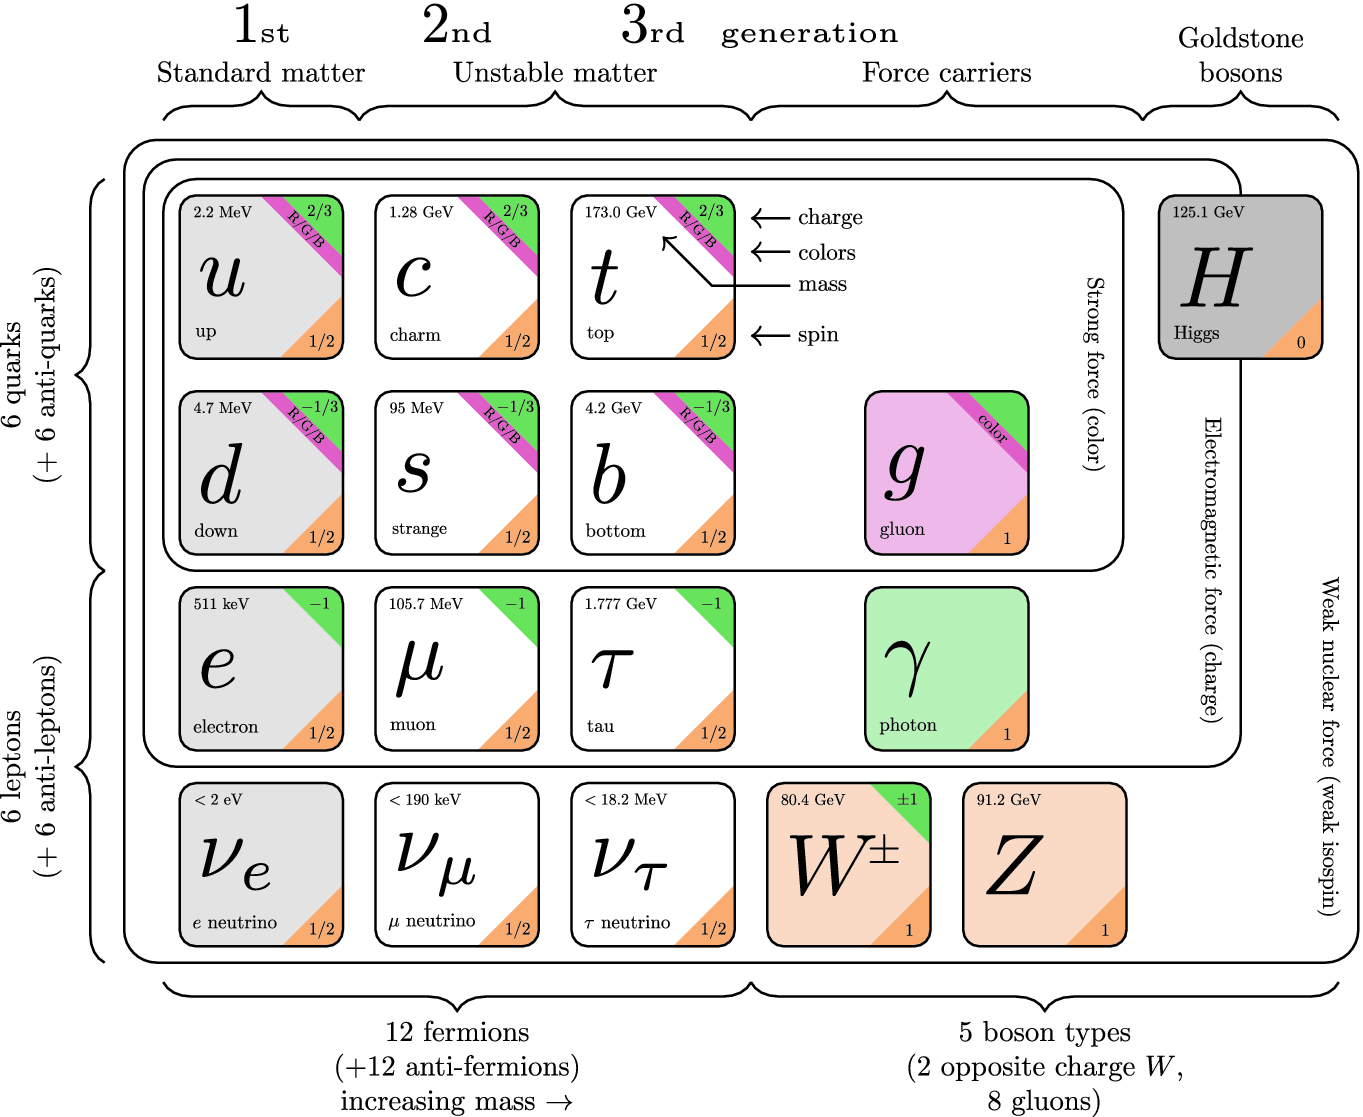
\includegraphics[width=5.2cm, height=4cm]{figs/SMFermions.png}
\end{center}
\end{figure} \vfill

However, \alert{this model has some fundamental shortcomings}, such as the possible existence of exotic particles which do not fit within this model (such as dark matter), therefore extensively searched for nowadays. \vfill
\end{frame}

\begin{frame}{At the origins of dark matter I}
\justifying
The concept of dark matter can be traced back to the 19th century, and \alert{was introduced to explain several astrophysical evidences}, among which: \vfill

\vspace{10pt}	
\begin{block}{ \centering Zwicky's calculations}\end{block}

\begin{itemize}
\justifying
\item Measurement of the mass of the Coma Cluster using the virial theorem;
\item Concluded that its mass was \textbf{400-500 times larger} than the value obtained by Hubble, considering only visible galaxies\footnote[frame]{These numbers were later proven to overestimated, but the idea behind the calculations is still accepted}. %\cite{Zwicky}.
\end{itemize} \vfill

\vspace{10pt}	
\begin{block}{ \centering Spiral galaxies rotation curves}\end{block}

\begin{columns}
	\begin{column}{0.65\textwidth}
\begin{itemize}
\justifying
\vspace{-5pt}	
\item Stars within spiral galaxies should rotate with a velocity depending on the radius to the galactic center, but \textbf{this is not what is observed experimentally}.% \cite{RotationCurves};
\vspace{1pt}	
\item Either our understanding of gravity at large scales or our basic understanding of galaxies as celestial bodies made of stars has to be revised.
\end{itemize} 
\end{column}

\begin{column}{0.44\textwidth}
\begin{figure}[htbp]
\begin{center}
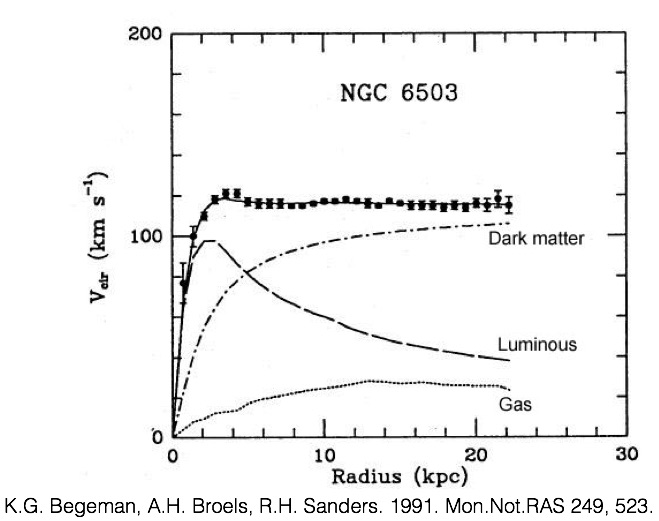
\includegraphics[width=4.5cm, height=3.7cm]{figs/RotationCurve.jpeg}
\end{center}
\end{figure}
\end{column}
\end{columns} \vfill

\end{frame}

\begin{frame}{At the origins of dark matter II}
\justifying

\vspace{5pt}
\begin{block}{ \centering CMB anisotropies}\end{block}

\begin{itemize}
\justifying
\item Background of primary radio waves emitted when the Universe became transparent around 380 000 years after the Big Bang;
\item Can be considered as emitting a black body spectrum with a temperature of $(2.72548\pm 0.00057)$K, but small anisotropies at the $10^{-5}$ level are observed;% \cite{CMBTemperature};
\item Implies that dark matter \textbf{accounts for $\sim 27\%$ of the total mass of the Universe}.
\end{itemize} \vfill

\begin{columns}
	\begin{column}{0.54\textwidth}
\begin{figure}[htbp]
\begin{center}
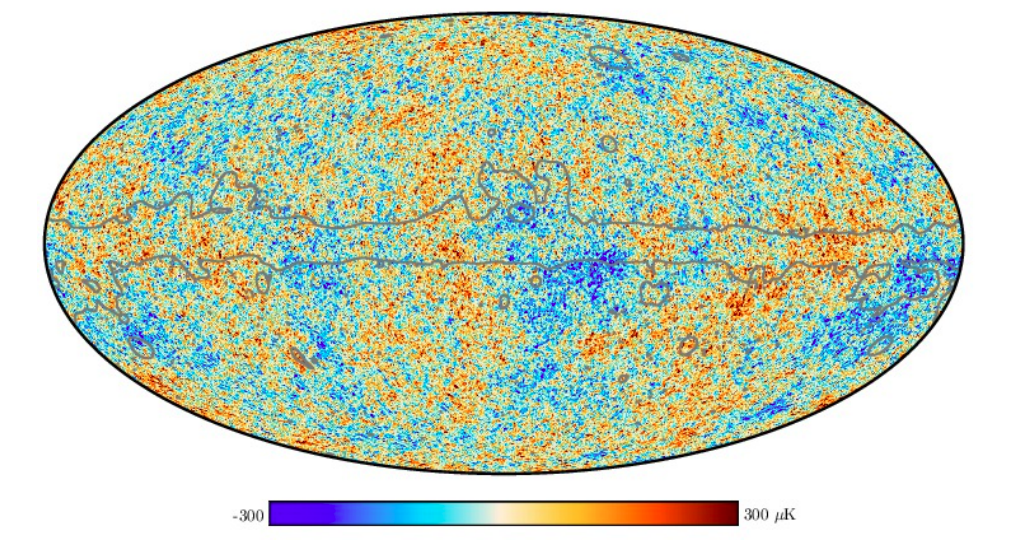
\includegraphics[width=6.5cm, height=3cm]{figs/PlanckTemperature.png}
\end{center}
\end{figure}
\end{column}
\begin{column}{0.44\textwidth}
\begin{figure}[htbp]
\begin{center}
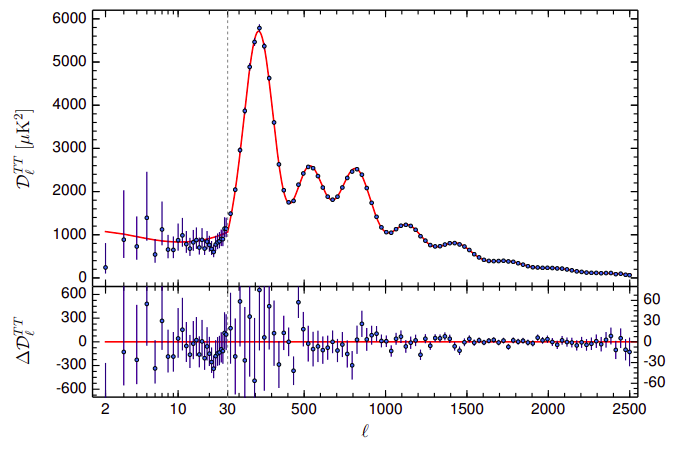
\includegraphics[width=5cm, height=3.5cm]{figs/PlanckSpectrum.png}
\end{center}
\end{figure}
\end{column}
\end{columns} \vfill

Other observations, such as the gravitational lensing effect, \alert{also tend to further support the existence of dark matter} (cf. backup). \vfill
\end{frame}

\begin{frame}{Dark matter properties}
\justifying

\alert{Several fundamental properties of dark matter} are nowadays known or assumed:

\begin{itemize}
\justifying
\item Dark matter \textbf{is a particle}, assumed to have a certain mass;
\item It should be \textbf{dark}, unable to interact with electromagnetic radiation, otherwise we would have seen it already. It should then also be \textbf{electrically neutral};
\item It is \textbf{non-baryonic}, because the energy density for the baryonic matter estimated from the CMB is too low to account for dark matter;
\item We only consider \textbf{cold dark matter} since the widely accepted $\Lambda_{CDM}$ model is based on this assumption and this can explain the large scale structures in the Universe;
\item It should \textbf{have a mass in the electroweak scale}, between 10 GeV and 1 TeV, because of the relic density obtained from the thermal freeze-out mechanism;% \cite{Freezeout1}.
\item Finally, it should be \textbf{long-lived}, since we expect that it has been produced during the Big Bang and is still present in the Universe.
\end{itemize}

\end{frame}

\begin{frame}{Dark matter searches}
\justifying

\vspace{5pt}
\begin{block}{ \centering Weakly Interactive Massive Particles}\end{block} \vfill
The \alert{WIMPs are the dark matter candidates} considered in this work, because of the so-called \textbf{WIMP miracle}. Indeed, they:

\begin{itemize}
\justifying
\item Are expected to interact very weakly with ordinary baryonic matter;
\item Have a mass in the 100 GeV-1 TeV range for reasonable electroweak production cross-section values;
\item Give us a dark matter candidate while being able to solve the \textbf{hierarchy problem}.
\end{itemize} \vfill

\vspace{5pt}
\begin{block}{ \centering Main search strategies}\end{block} \vfill

\begin{columns}
	\begin{column}{0.45\textwidth}
\begin{figure}[htbp]
\begin{center}
\begin{figure}[htbp]
\begin{center}
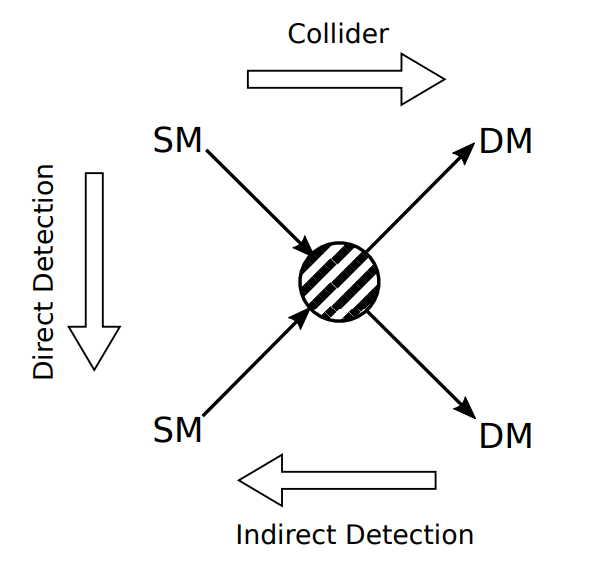
\includegraphics[width=4.2cm, height=3.5cm]{figs/ThreeWays.png}
\end{center}
\end{figure}
\end{center}
\end{figure}
\end{column}
\begin{column}{0.54\textwidth}
\alert{Different search strategies} are used:

\begin{itemize}
\justifying
\item The \textbf{direct and indirect searches}, relying on the production of baryonic
matter from the interaction between two DM particles or on the observation of the interaction
between the dark and baryonic sectors;
\item And the \textbf{collider production}, able to probe lower dark matter candidates masses.
\end{itemize}

\end{column}
\end{columns} \vfill
\end{frame}

\begin{frame}{Focus of this thesis I}
\justifying
We are searching for \alert{dark matter produced in association with either one or two top quarks}. Several \textbf{simplified models} have been considered:

\begin{itemize} 
	\justifying
	\item Spin 1/2 DM $\chi$ (mass $\in [1, 55]$ GeV, Dirac fermion) \\
	\item Spin 0 scalar (S)/pseudoscalar (PS) mediator $\phi$/a (Yukawa-like structure of such interactions $\rightarrow$ \textbf{gain from the coupling of the mediator to top quarks}) \\
	\item Mediator mass $\in [10, 1000]$ GeV \\
	\item Coupling $g_{\chi}$ mediator/DM set to 1 (same for all $g_q$ couplings) \\
	%\item Most samples cross-section at NLO
	%\item No mixing between $\phi$ and the SM Higgs boson
\end{itemize}\vfill

\begin{center}
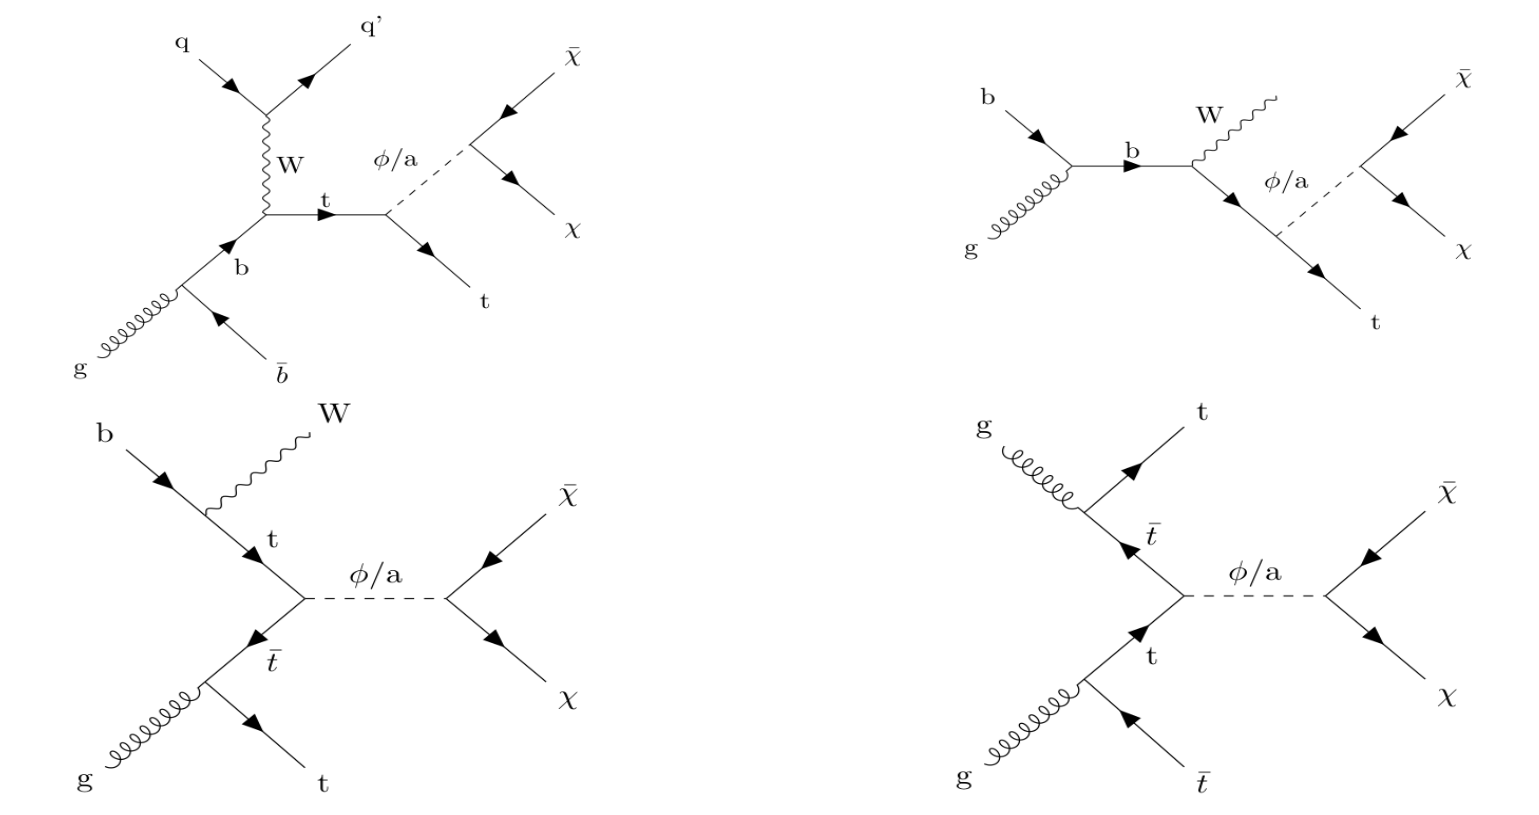
\includegraphics[width=0.78\textwidth, height=140pt]{figs/AllFeynman.png}
\end{center}

%\begin{columns}
%	\begin{column}{0.675\textwidth}
%		\begin{center}
%			\begin{block}{ \centering $t/ \bar t$+DM tW models}\end{block}	
%			%\alert{\textbf{$t$ + DM models}} \\ \vspace{5pt}
%			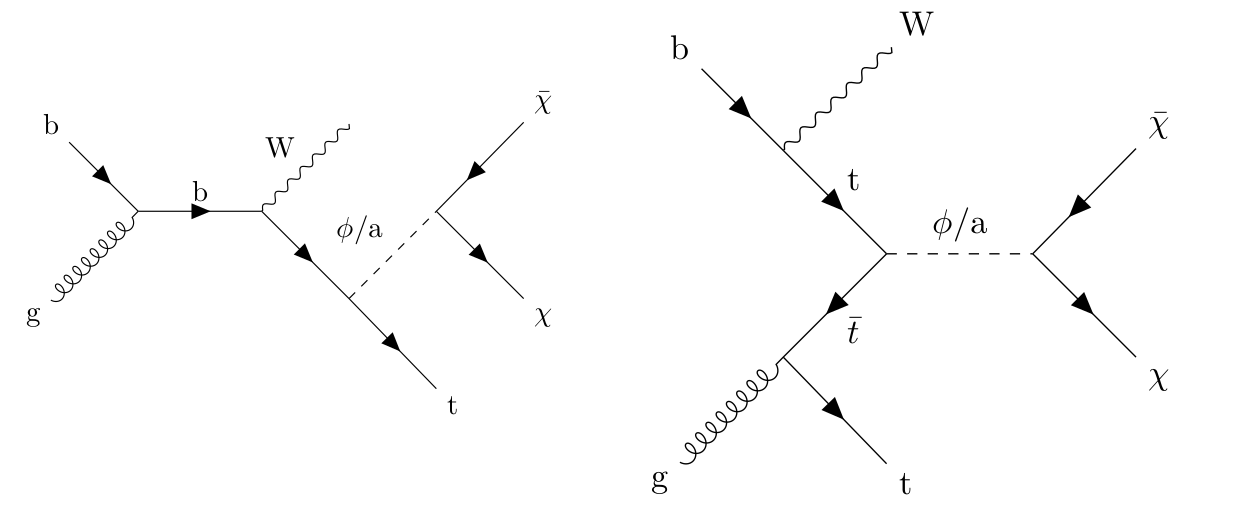
\includegraphics[width=1.0\textwidth]{figs/feynman_tDM_mine.png}
%    		 \end{center}
%	\end{column} \hfill
%	\begin{column}{0.3\textwidth}
%		\begin{center}
%			\begin{block}{\centering $t \bar t$+DM model}\end{block}				
%			%\alert{\textbf{$t \bar t$ + DM model}} \\ \vspace{5pt}
%			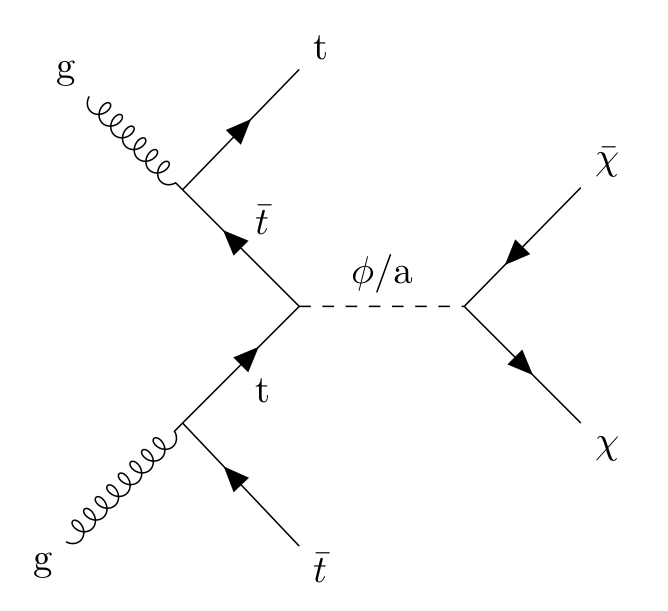
\includegraphics[width=1.0\textwidth]{figs/feynman_ttDM_mine.png}
%    		 \end{center}
%	\end{column} \hfill
%\end{columns} \vfill

%The Yukawa coupling typically favors searches for dark matter \textbf{produced in association with heavy quarks} such as this one. Such MET+X are heavily depend on the MET spectrum, which is expected to be larger for the signals than most backgrounds. \vfill
\end{frame}

\begin{frame}{Focus of this thesis II}
\justifying
The \alert{typical final state} of such topology is made out of:
\begin{itemize}
\justifying
\item 1 or 2 bottom quarks coming from the decay of the top quark(s);
\item 2 W bosons, seen as a combination of jets and leptons depending on the channel, produced directly or coming from the decay of the top quarks ($t \rightarrow b + W$);
\item Some missing transverse energy coming from the dark matter and the neutrinos from the leptonic decay of the Ws.
\end{itemize} \vfill

In particular, we are studying the \alert{dilepton final state} in this work: 
\begin{itemize}
\justifying
\item Has the lowest branching ratio: BR($W^+ \rightarrow l^+ + \nu_l) = (10.80 \pm 0.09)\%$ for each of the charged leptons (contains only $\sim 5\%$ of the signal events);
\item But, electrons and muons can usually be reconstructed better than jets, leading to lower systematic uncertainties (taus are not considered directly in this work);
\item And this channel has the lowest number of backgrounds, with cross-sections typically lower, resulting in a better signal isolation.
\end{itemize} \vfill

%This channel is then \textbf{expected to be competitive with the hadronic and semileptonic channels}, especially when considering high mediator masses, which feature a higher global signal/background discrimination. \vfill
\end{frame}

\begin{frame}{Previous relevant results I}
\justifying
\vspace{5pt}
A \alert{similar analysis was carried out by CMS} using 2016 data, considering only the $t \bar t$+DM signal and the dilepton final state (EXO-17-014). \vfill % \cite{PreviousDoubleTopAllLep13CMS}. \vfill

%\vspace{-10pt}
%\begin{figure}[htbp]
%\begin{center}
%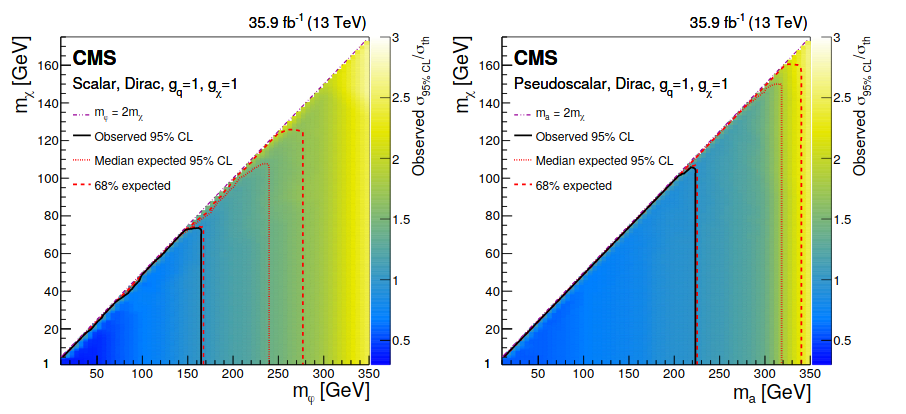
\includegraphics[width=11cm, height=4.8cm]{figs/CMSttbarExclusion.png}
%\end{center}
%\end{figure} \vfill

\begin{figure}[htbp]
\centering
\begin{minipage}[b]{.49\textwidth}
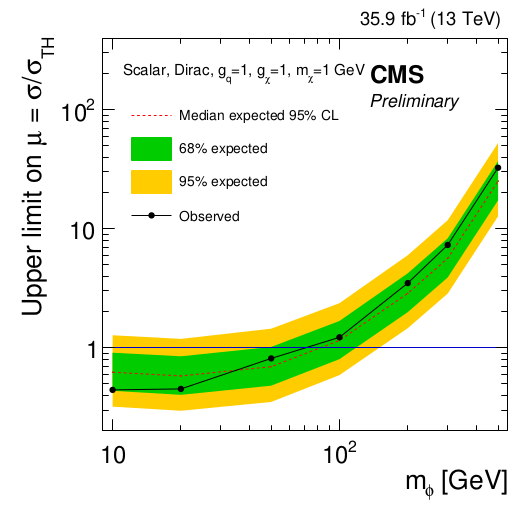
\includegraphics[width=5.4cm, height=4.7cm]{figs/Juan_S.png}
\end{minipage}\hfill
\begin{minipage}[b]{.49\textwidth}
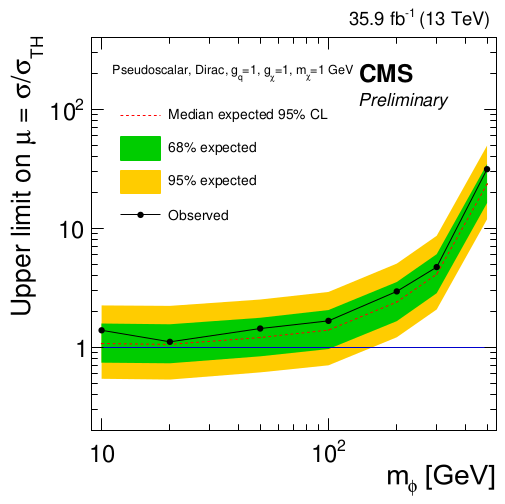
\includegraphics[width=5.4cm, height=4.7cm]{figs/Juan_PS.png}
\end{minipage}\hfill
\label{fig:Juan}
\end{figure}

This analysis \textbf{excluded scalar mediators} with masses below 80 GeV, while \textbf{no exclusion was achieved} when considering pseudoscalar mediators. \vfill
A \alert{combination of the three possible final states} (hadronic, semileptonic and dileptonic) was also performed by CMS (EXO-16-049). \vfill

%The observed (expected) limits \textbf{excluded a pseudoscalar mediator} with mass below 220 (320) GeV, and \textbf{a scalar mediator} with mass below 160 (240) GeV. \vfill
%This provided the \alert{most stringent constraints} ever obtained at the time on the scalar dark matter mediator model. \vfill
\end{frame}

\begin{frame}{Previous relevant results II}
\justifying
\vspace{5pt}
A \alert{combination of both the $t/ \bar t$+DM and $t \bar t$+DM processes} has also been performed by CMS (EXO-18-010). The inclusion of the single top signal process \textbf{improved up to a factor 2} the limits obtained by the $t \bar t$ analysis on its own. This analysis: %\cite{PreviousSingleDoubleTopAllLep13CMS}. 

\begin{itemize}
\item Only considered the 2016 data-taking period;
\item And only considered the semileptonic and hadronic final states.
\end{itemize} \vfill

\begin{center}
\begin{columns}
	\begin{column}{1.0\textwidth}
		\begin{center}
			%\begin{block}{\centering $t \bar t$+DM limits}\end{block}				
			%\alert{\textbf{$t \bar t$ + DM model}} \\ \vspace{5pt}
			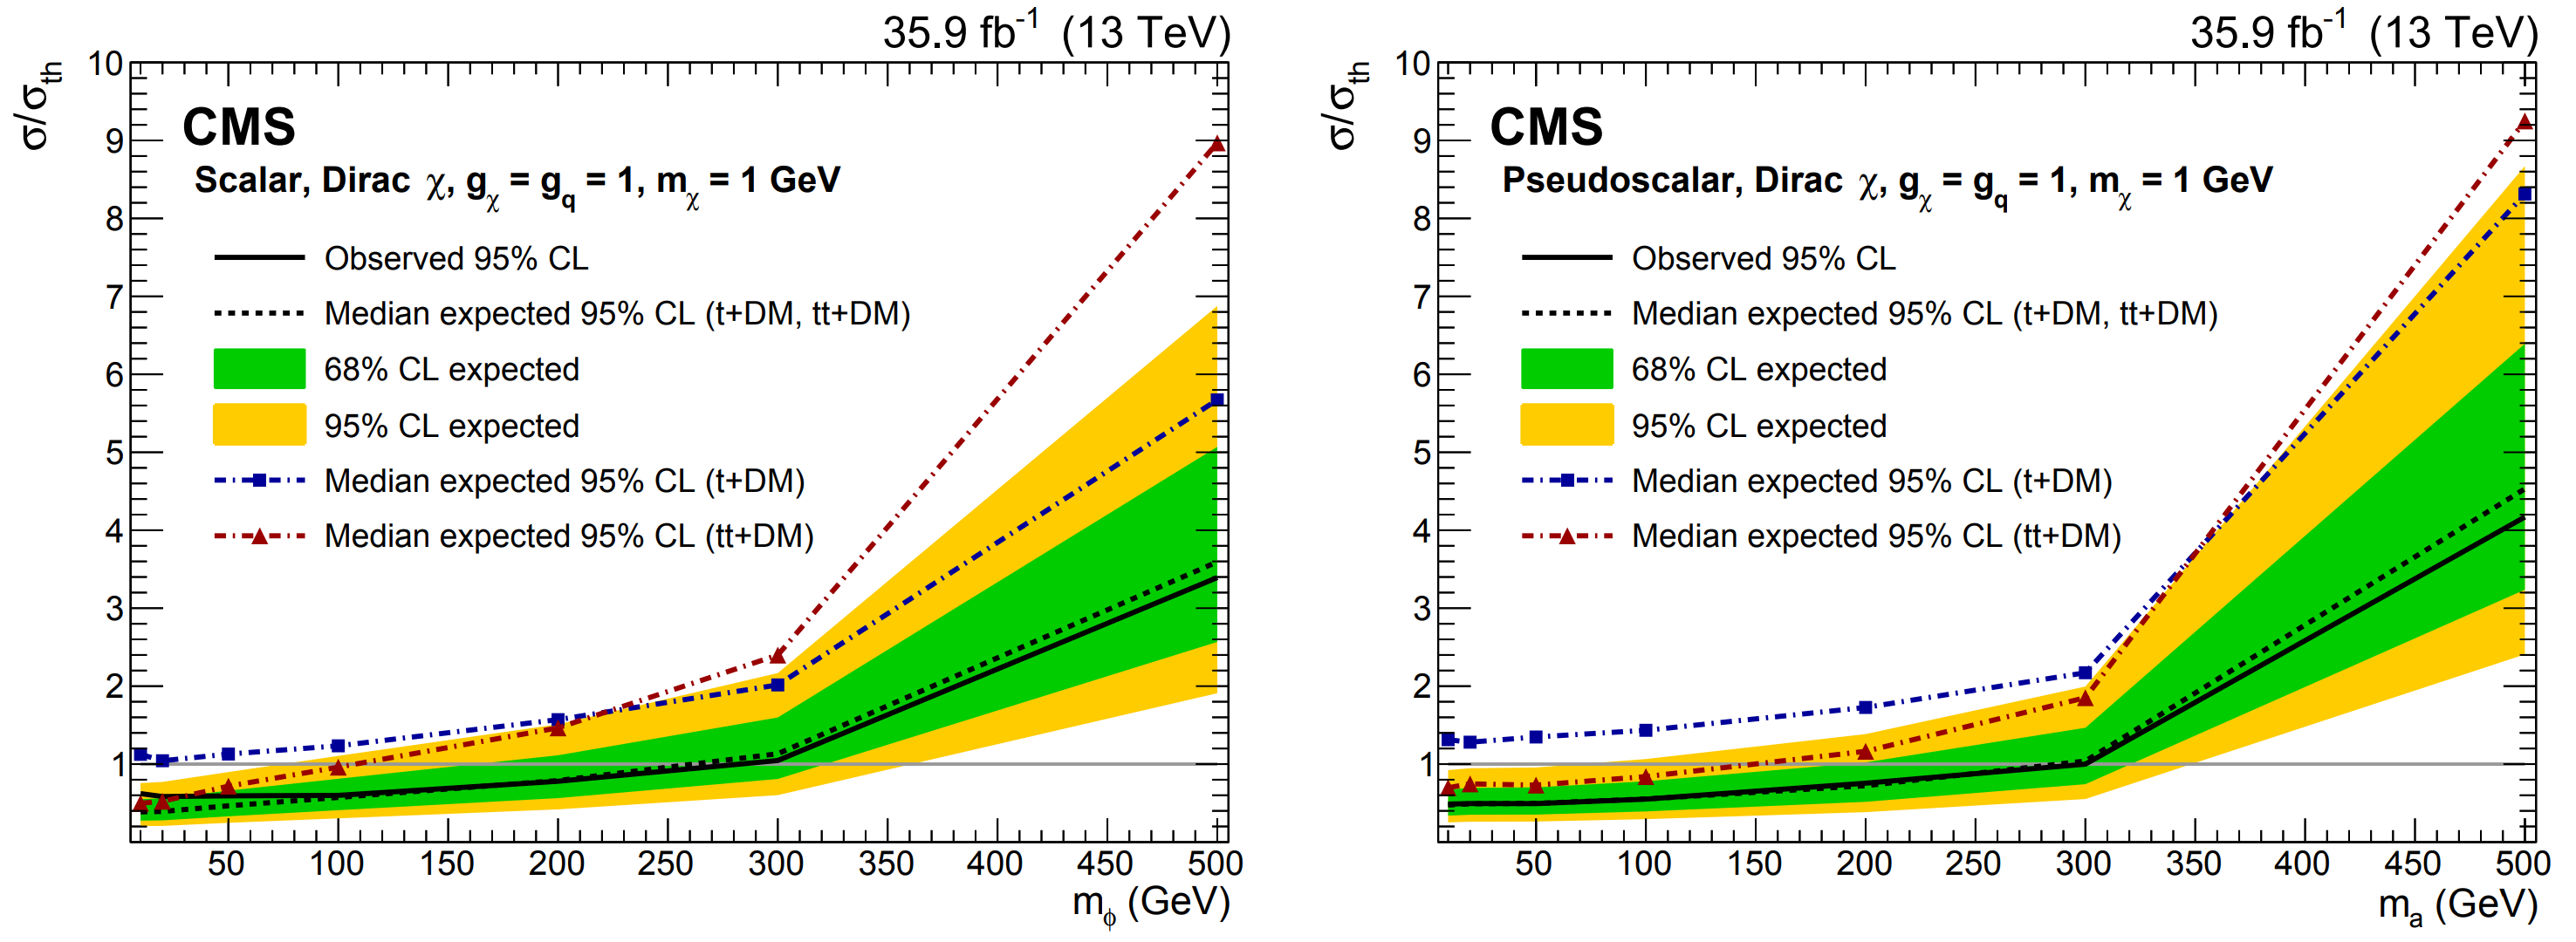
\includegraphics[width=1.0\textwidth]{figs/limitsprevious.png}
    		 \end{center}
	\end{column} \hfill
\end{columns}
\end{center} \vfill

Scalar (pseudoscalar) mediators were with this combination \textbf{excluded up to 290 (300) GeV} at the 95\% confidence level. \vfill %The inclusion of the full Run II dataset and the dilepton final state \textbf{is expected to improve these results}.
\end{frame}

\begin{frame}{Previous relevant results III}
\justifying
The \alert{ATLAS collaboration also obtained exclusion limits} using the full Run II legacy dataset and considering the $t \bar t$+DM dilepton final state only (ATLAS-CONF-2020-046). \vfill

 \begin{figure}[htbp]
\centering
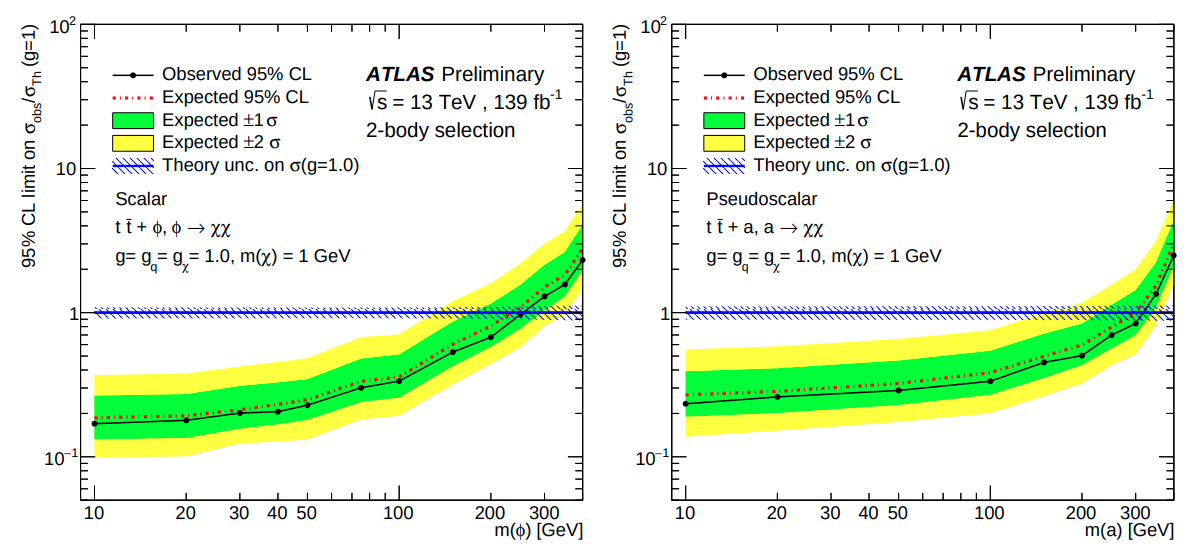
\includegraphics[width=10.5cm, height=4.7cm]{figs/ATLASICHEP.png}
\end{figure} \vfill

They obtained \textbf{expected scalar (pseudoscalar) exclusion limits of 250 (300) GeV}, by using NLO cross-sections for the signals, around 20-30\% higher than ours. \vfill
\end{frame}


















\begin{frame}[standout]
The experimental setup
\end{frame}

\begin{frame}{The Large Hadron Collider}
\justifying
The data analyzed \alert{has been taken by the Large Hadron Collider}:

\begin{columns}
	\begin{column}{0.55	\textwidth}
	\begin{itemize}
\justifying
\item A \textbf{27 km circular underground proton-proton collider}, located at CERN;
%\item Built in order to study and reproduce the conditions of the Universe at its origin;
\item Provided the collisions that led to the discovery of the Higgs boson in 2012;% \cite{HiggsDiscovery1, HiggsDiscovery2};
\item Currently the most powerful accelerator in the world with its $pp$ center of mass energy $\sqrt{s} = 13$ TeV, therefore able to \textbf{scan new parts of the phase space}.
\end{itemize}
	\end{column}
	\begin{column}{0.48\textwidth}
	\begin{figure}[htbp]
\begin{center}
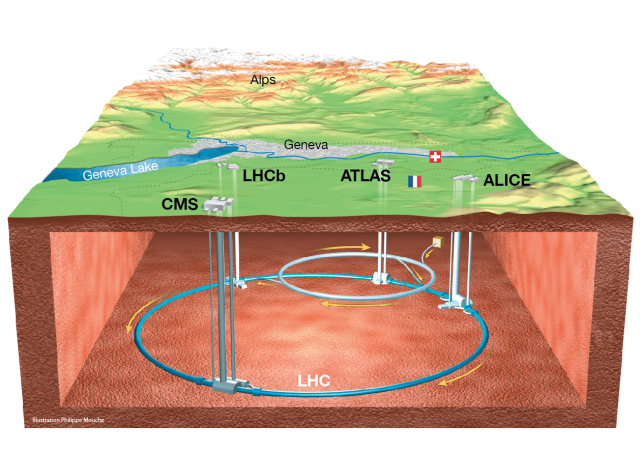
\includegraphics[width=5cm, height=3.6cm]{figs/LHCunderground.png}
\end{center}
\end{figure}
	\end{column}
\end{columns} \vfill

\vspace{10pt}
The data considered in this work has been collected during the \textbf{Run II of operation of the LHC} (from 2016 to 2018), at 13 TeV, totaling ($137.1 \pm 2.0$)~fb$^{-1}$ of data, selected by the different levels of trigger from the 40 MhZ collision rate. \vfill
\end{frame} 

%\begin{frame}{The Large Hadron Collider II}
%\justifying
%In the 4 interaction points of the LHC, \alert{4 detectors} have been placed: ATLAS, CMS, ALICE and LHCb, each having their own characteristics and features: \vfill
%
%\begin{columns}
%	\begin{column}{0.40	\textwidth}
%\begin{center}
%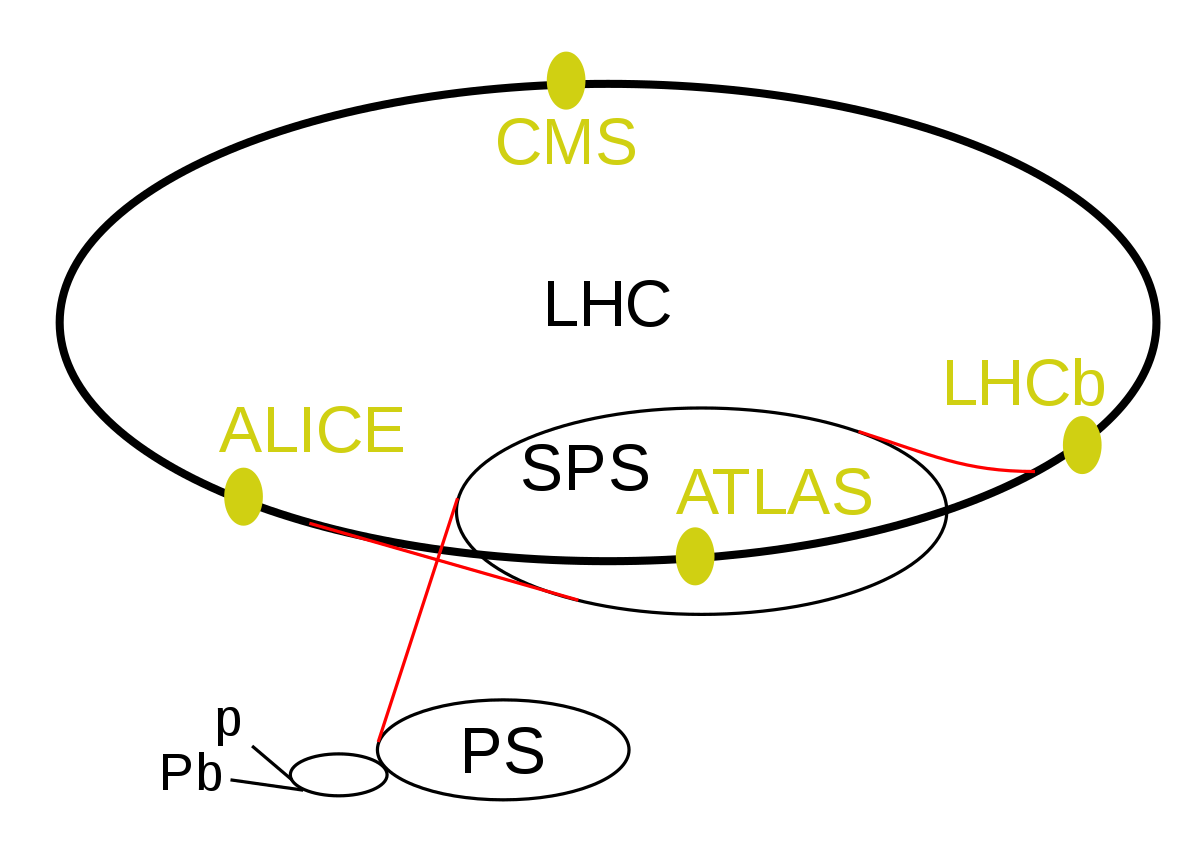
\includegraphics[width=5cm, height=3.6cm]{figs/LHCdetectors.png}
%\end{center}
%\end{column}
%\begin{column}{0.58	\textwidth}
%\begin{itemize}
%\justifying
%\item ATLAS and CMS are \textbf{general purpose detectors}, able to study exotic processes such as well as able to to make precision measurements on Standar Model physics;
%\item ALICE is mostly dedicated to the study of the quark-gluon plasma originating from heavy ions collisions;
%\item And LHCb has been designed to study the CP violation phenomena, which could be the sign of some new physics.
%\end{itemize}
%\end{column}
%\end{columns} \vfill
%
%\vspace{10pt}
%The collisions analyzed in this work \alert{have been collected by the CMS detector}. \vfill
%\end{frame}

\begin{frame}{The CMS detector I}
\justifying

\begin{columns}
\begin{column}{0.56	\textwidth}
\justifying
The \alert{Compact Muon Solenoid} is one of the two \textbf{general purpose detectors} of the LHC. Its main objectives consist in:
\begin{itemize}
\justifying
\item Make precision measurements;
\item Searching for and studying the properties of the Higgs boson;
\item Trying to discover new BSM physics, such as the possible existence of dark matter.
\end{itemize}
\end{column}
\begin{column}{0.40	\textwidth}
\begin{center}
\includegraphics[width=4.7cm, height=3.5cm]{figs/CMSphoto.jpg}
\end{center}
\end{column}
\end{columns} \vfill

In a nutshell, CMS:
\begin{itemize}
\justifying
\item Is a relatively \textbf{compact} (14.000 tons, distributed over a diameter of 15 meters and a length of 8 meters) cylindrical detector; 
\item Is made out of a central part with cylindrical shape, the barrel, and two endcaps, one on each side in order to be \textbf{as hermetic as possible}, covering all the possible angles around the beam pipe;
\item Has a \textbf{large solenoid} as middle piece, able to produce a 3.8 T field;
\item Features a \textbf{powerful tracker and muon detection system}.
\end{itemize} \vfill
\end{frame}

\begin{frame}{The CMS detector II}
\justifying
The CMS detector is also \alert{made out of different layers}, each having its own purpose, allowing to identify unequivocally each particle created and measure their properties, thanks to the reconstruction performed by the Particle Flow algorithm. \vfill

\begin{figure}[htbp]
\begin{center}
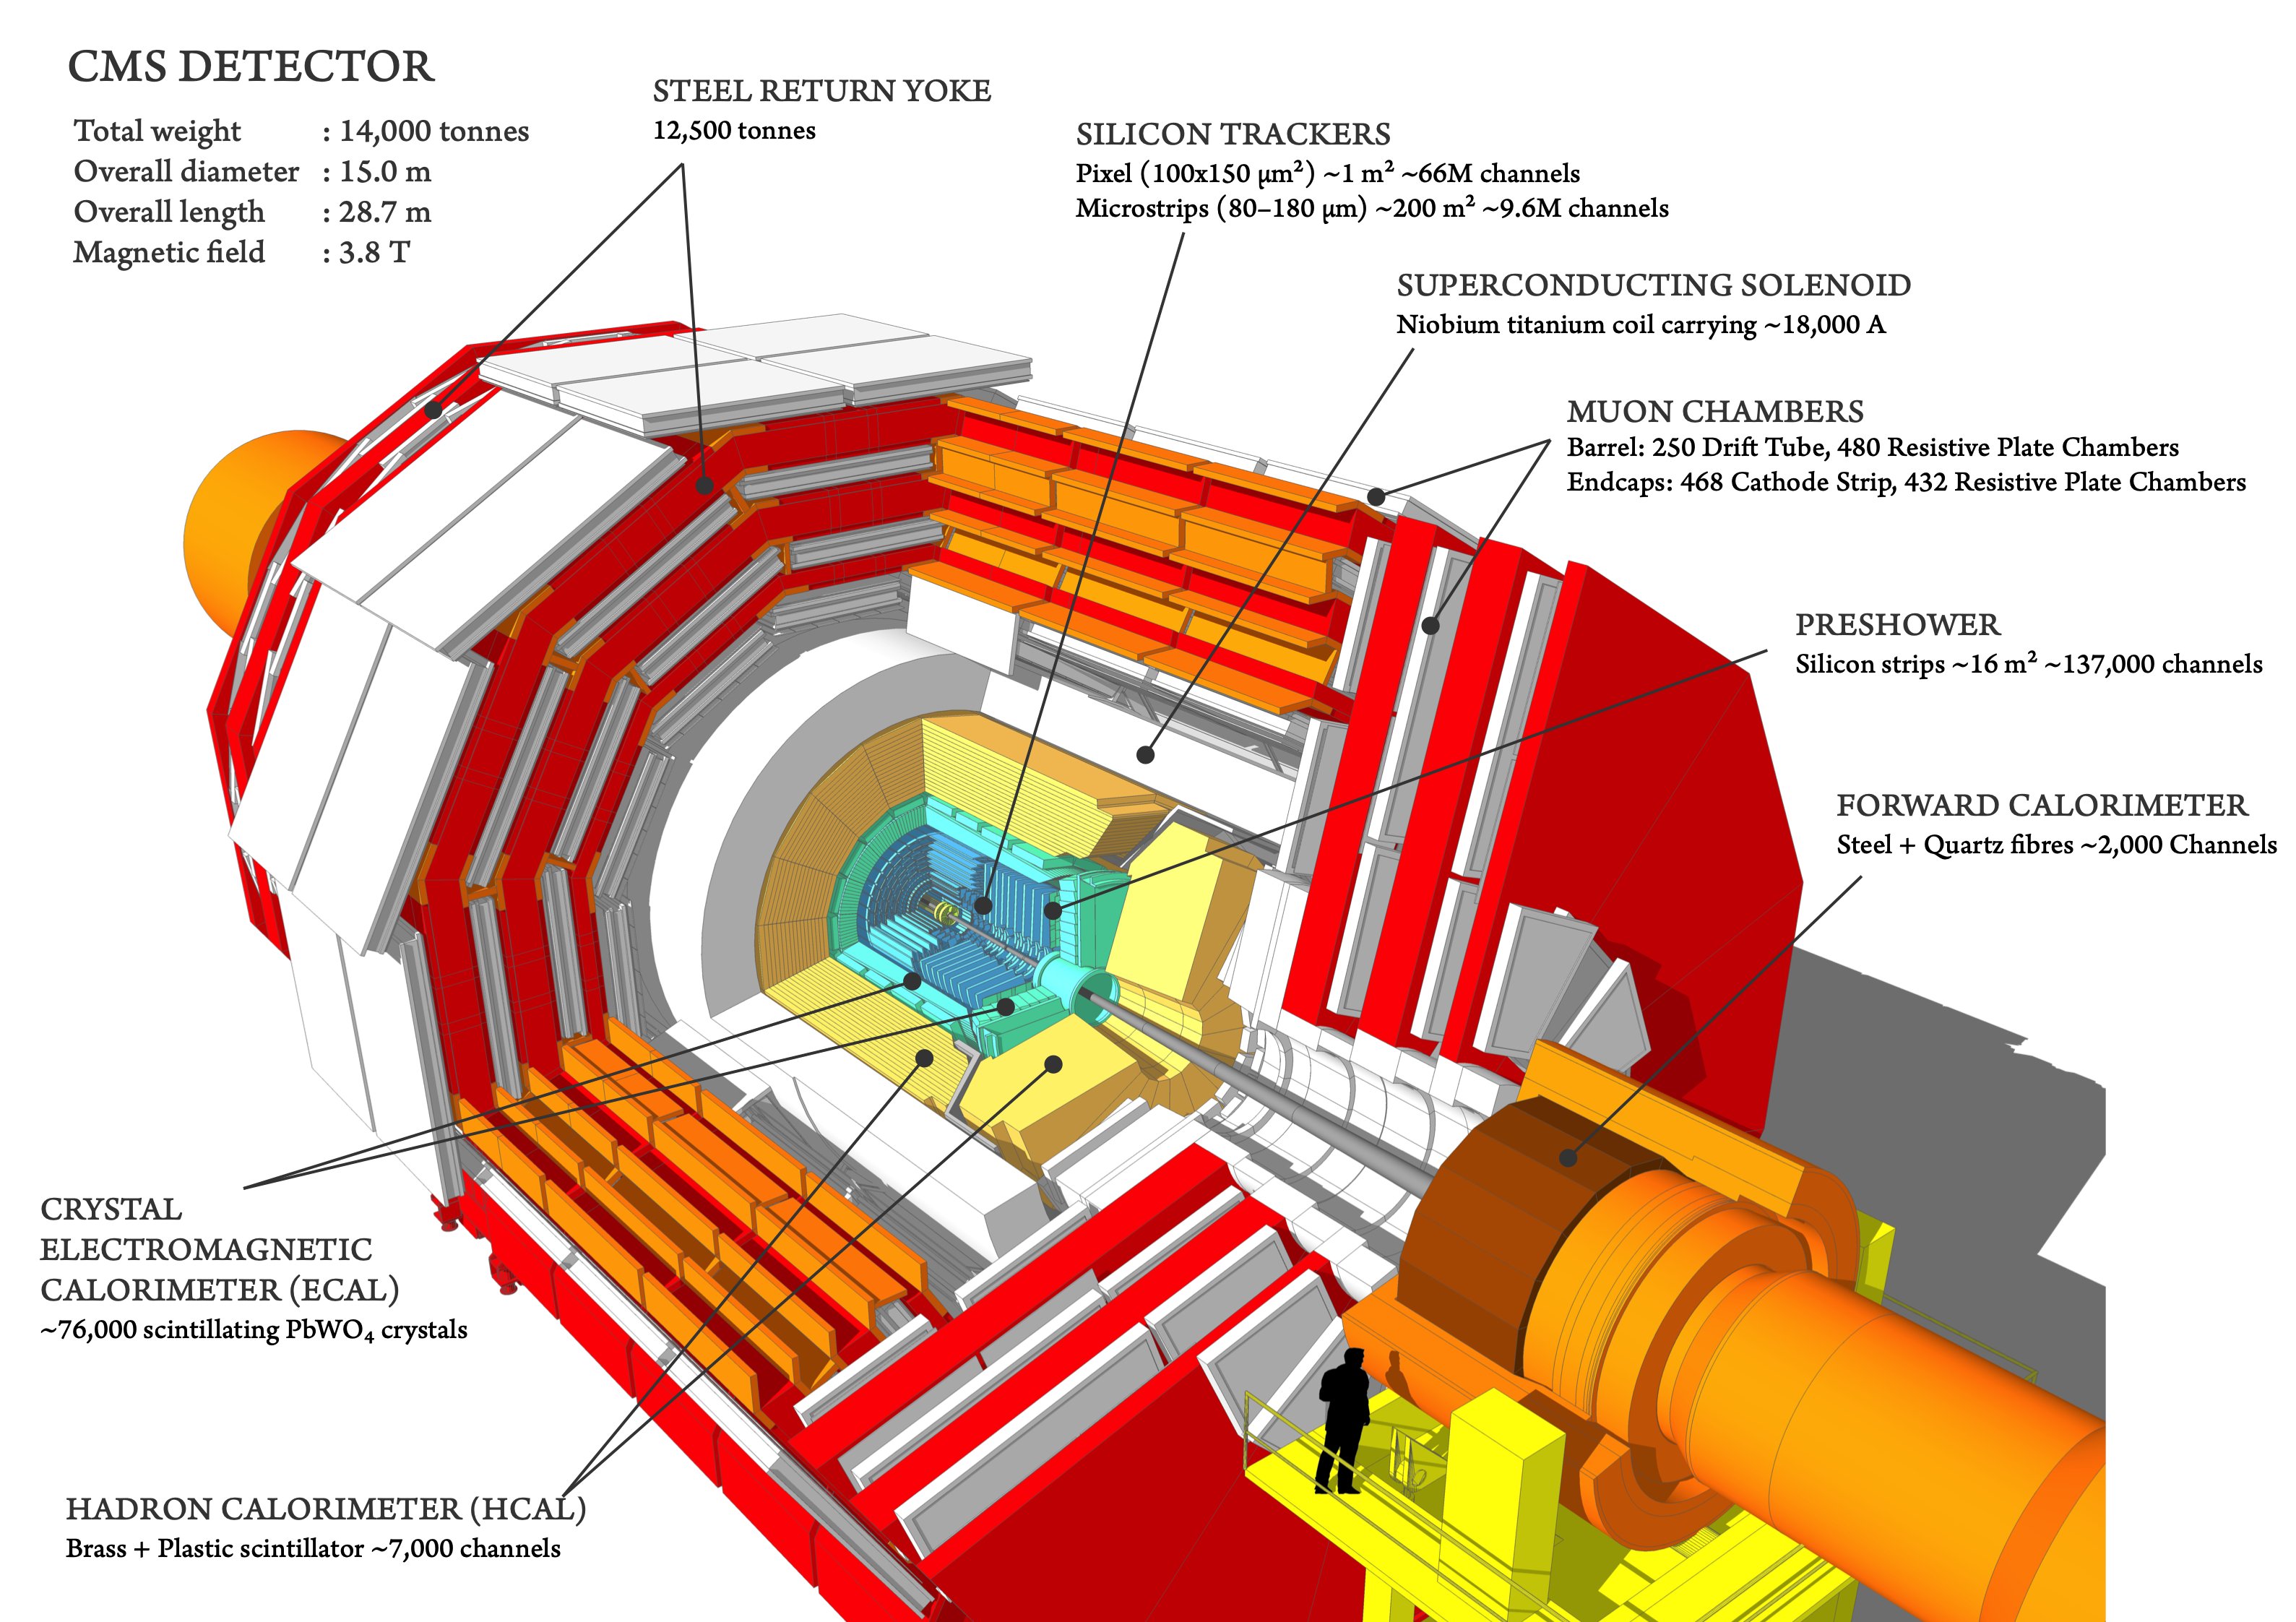
\includegraphics[width=9cm, height=6cm]{figs/CMS.png}
\end{center}
\end{figure} \vfill
\end{frame}

\begin{frame}{The CMS detector III}
\justifying
Each subdetector of CMS has been \alert{designed carefully to fulfill a specific purpose}:

\begin{itemize}
\justifying
\item The \textbf{tracker} is the innermost piece of CMS, able to reconstruct the trajectories of charged particles issued from the primary and secondary interaction vertices in a quick and precise way;
\item The \textbf{Electromagnetic Calorimeter}, enclosing the tracker system and able to give information about the energy of electrons and photons;
\item The \textbf{Hadronic Calorimeter}, able to measure the energy of incident hadrons from the ionization process happening in its core;
\item The 12.5 meters long and 6 meters large \textbf{solenoid}, allowing to measure precisely the charge and momentum of particles produced using the Lorentz effect, by measuring the curvature of their tracks;
\item And finally, the \textbf{muon system}, covering more than 25 000 m$^2$ and made out of three different subsystems:

\begin{itemize}
\justifying
\item The \textbf{Drift Tubes} (DTs), in the barrel region;%, where the flux of muons is low and where the magnetic field is mostly uniform;
\item The \textbf{Cathode Strip Chambers} (CSCs) in the two endcaps;%, where the muon rates and background levels are much larger and where the magnetic field is large and non-uniform;
\item And the \textbf{Resistive Plate Chambers} (RPCs), mostly added to the barrel and to the endcap regions in order to cope with (in)ability of  the previous muon system to identify unequivocally the correct bunch crossing when the LHC is running at full luminosity.
\end{itemize}

\end{itemize}
\end{frame}


















\begin{frame}[standout]
Analysis context
\end{frame}

\begin{frame}{Analysis context}
\justifying
Run II legacy paper being worked on, expected to \alert{combine both the $t/\bar t$+DM and $t \bar t$+DM searches}, and the 3 possible final states (hadronic, semileptonic and dileptonic). \\
\hspace{10pt} $\rightarrow$ Pre-approval process expected to start within a few weeks. \vfill

The effort is \textbf{globally common} between the groups (Wisconsin, DESY, IFCA) studying the three different final states:
\begin{itemize}
\justifying
\item Objects are defined in a common way;
\item Control and signal region orthogonal between the channels.\\
$\rightarrow$ Number of leptons and b-jet categorization to improve the sensitivity by defining enriched $t/\bar t$+DM and $t \bar t$+DM regions.
\end{itemize} \vfill

This talk will however \textbf{be focused on the dilepton final state} only. \vfill
\begin{block}{}
\begin{center}
All the results presented here have not been published yet, but have been fully endorsed by the MET+X conveners of the CMS collaboration.
\end{center}
\end{block} \vfill
\end{frame}
















%\begin{frame}[standout]
%Hadronic final state \\
%Semileptonic final state
%\end{frame}
%
%\begin{frame}{Event selection}
%\justifying
%\begin{columns}
%		\hspace{5pt}
%		\begin{column}{0.64\textwidth}
%			\begin{center}
%				%\begin{block}{\centering Leading $p_T$}\end{block}	
%				%\alert{Leading $p_T$} \\ \vspace{5pt}
%     			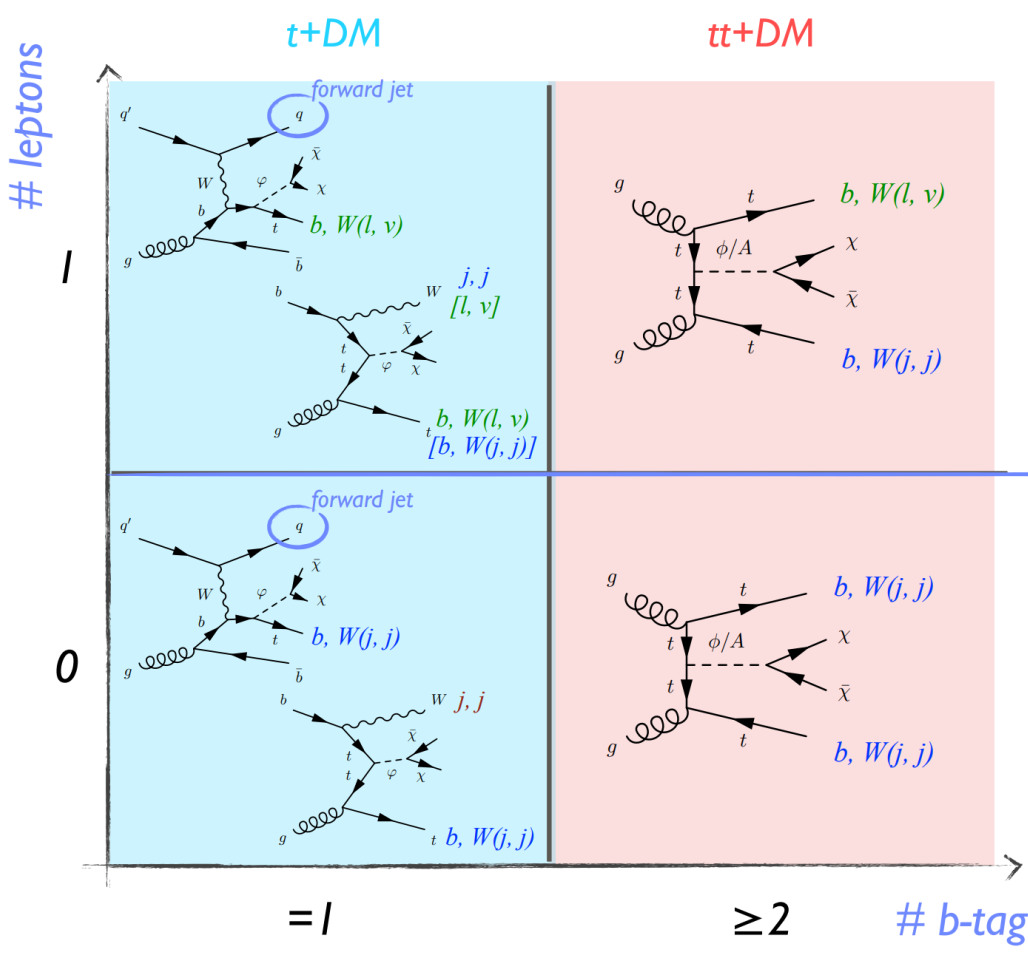
\includegraphics[width=\textwidth]{figs/semiHadronicSelection.png}
%    		\end{center}		
%		\end{column} \hfill
%		\begin{column}{0.39\textwidth}
%			\begin{center}
%				\begin{block}{\centering Single lepton}\end{block} \vfill
%				\begin{itemize}
%				\item Single lepton trigger
%				\item 1 isolated lepton (e, $\mu$)
%				\item $\geq 2$ jets
%				\item MET $> 160$ GeV
%				\item + $0, \geq 1$ forward jets ($|\eta|> 2.4$)
%				\end{itemize} \vfill
%				
%				\vspace{10pt}
%				\begin{block}{\centering All hadronic}\end{block} \vfill	
%				\begin{itemize}
%				\item MET trigger
%				\item Leptons veto (e, $\mu$)
%				\item $\geq 3$ jets
%				\item MET $> 250$ GeV
%				\item + $0, \geq 1$ forward jets
%				\end{itemize} \vfill
%    		\end{center}		
%		\end{column} \hfill
%\end{columns}
%\end{frame}





















\begin{frame}[standout]
Samples and objects
\end{frame}

\begin{frame}{Data and MC samples}
\justifying
\begin{block}{\centering Data}\end{block}
\alert{Single/double leptons datasets} built to avoid any eventual double counting, considering the 3 years of the Run II of operation of the LHC:
\begin{columns}
\hspace{15pt}
	\begin{column}{0.32\textwidth}
		\begin{itemize}
		\item ($35.9 \pm 0.9$) fb$^{-1}$
		\end{itemize}
	\end{column} \hfill
	\begin{column}{0.32\textwidth}
		\begin{itemize}
		\item ($41.5 \pm 1.0$)~fb$^{-1}$
		\end{itemize}
	\end{column} \hfill
	\begin{column}{0.32\textwidth}
		\begin{itemize}
		\item ($59.7 \pm 1.5$)~fb$^{-1}$
		\end{itemize}
	\end{column} \hfill
\end{columns} \vfill
\vspace{5pt}
A \textbf{blinding policy} has been followed at first, allowing us to only look at $1$~fb$^{-1}$ of data per year near the signal regions. The \textbf{unblinding} was done with the analysis freezed and the green light received from the conveners. \vfill
\vspace{10pt}
\begin{block}{\centering Backgrounds}\end{block}
The \alert{major backgrounds have been mostly considered from MC}. Each year comes with its corresponding MC samples:

\begin{itemize}
\justifying
\item $t \bar t$: considering both its semileptonic and dileptonic decays;%, TuneCUETP8M2 (2016) and TuneCP5 (2017, 2018);
\item Single top: s, t and tW channels considered;
\item Drell-Yan: HT-binned samples to increase the statistics, with a correction factor derived from data applied;
\item $t\bar{t}Z$ and $t\bar{t}W$: usually grouped together as ttV, and considering both the hadronic and leptonic final states;
\item Others, such dibosons and tribosons production, all taken from MC directly.
\end{itemize} \vfill
\end{frame}

\begin{frame}{Signal samples}
\justifying
The \alert{signals samples have been generated} using MADGRAPH and PYTHIA8 (CP5 tune) at LO and simulated events are interfaced with a realistic model of the CMS detector using Geant4 and reconstructed using the official CMS reconstruction algorithms. \vfill
The $t/\bar t$+DM and $t \bar t$+DM processes are both considered:

\begin{itemize}
\item Both scalar and pseudoscalar mediators are considered;
\item 400.000 events were produced for each mediator mass, from 10 to 1000 GeV;
\item The dark matter mass was set to 1 GeV, but additional samples ranging from 1 to 55 GeV were also produced;
\item All the $g_q$ and $g_\chi$ couplings were set to 1.
\end{itemize} \vfill

\textbf{Recommended correction factors} (L1 ECAL prefiring in 2016 and 2017, HEM issue in 2018) are then applied to the simulation. \vfill 
$\rightarrow$ All the samples used and their cross-sections are listed in the backup. \vfill
\end{frame}

\begin{frame}{Signal samples distributions with normalization}
\justifying
\begin{block}{\centering $t/\bar t$+DM}\end{block} \vspace{-10pt}
\begin{figure}[htbp]
\centering
\begin{minipage}[b]{.49\textwidth}
\vspace{-5pt}
\begin{block}{\centering Scalar}\end{block}
\begin{center}
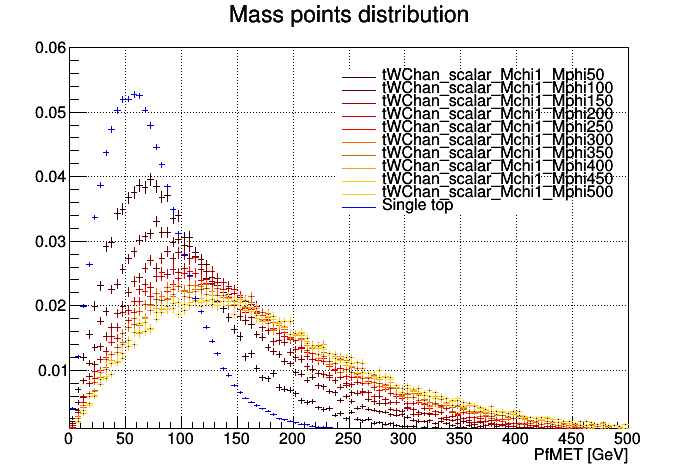
\includegraphics[width=5.2cm, height=3.5cm]{figs/singleTopScalarMETNorm.png}
\end{center}
\end{minipage}
\begin{minipage}[b]{.02\textwidth}\end{minipage}
\begin{minipage}[b]{.49\textwidth}
\vspace{-5pt}
\begin{block}{\centering Pseudoscalar}\end{block}
\begin{center}
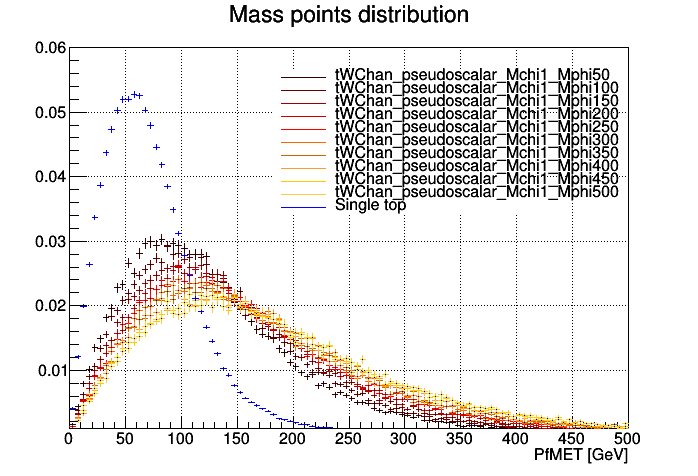
\includegraphics[width=5.2cm, height=3.5cm]{figs/singleTopPseudoMETNorm.png}
\end{center}
\end{minipage}
\end{figure} \vfill

\vspace{-5pt}
\begin{block}{\centering $t \bar t$+DM}\end{block} \vspace{-10pt}
\begin{figure}[htbp]
\centering
\begin{minipage}[b]{.49\textwidth}
\begin{center}
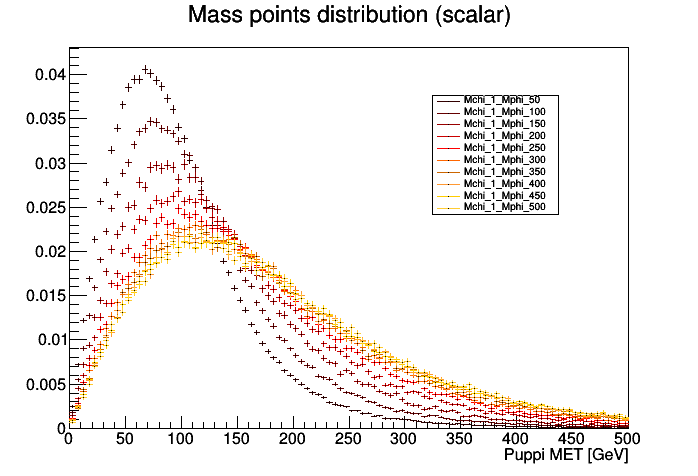
\includegraphics[width=5.2cm, height=3.5cm]{figs/scalarMETmChi1Norm.png}
\end{center}
\end{minipage}\hfill
\begin{minipage}[b]{.49\textwidth}
\begin{center}
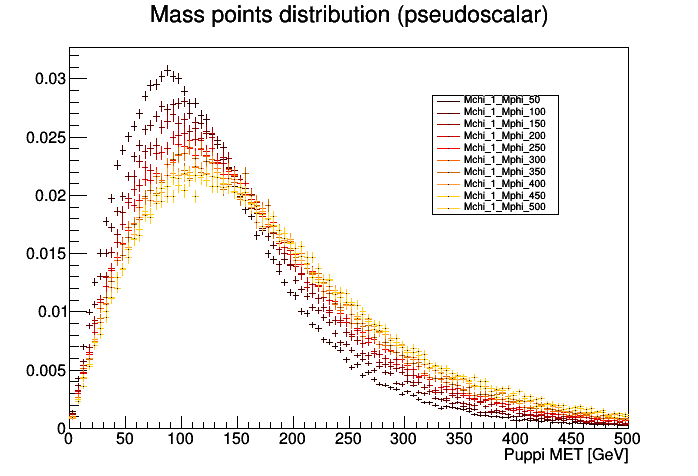
\includegraphics[width=5.2cm, height=3.5cm]{figs/pseudoscalarMETmChi1Norm.png}
\end{center}
\end{minipage} \hfill
\end{figure} \vfill
\end{frame}

\begin{frame}{Signal samples distributions without normalization}
\justifying
\begin{block}{\centering $t/\bar t$+DM}\end{block} \vspace{-10pt}
\begin{figure}[htbp]
\centering
\begin{minipage}[b]{.49\textwidth}
\vspace{-5pt}
\begin{block}{\centering Scalar}\end{block}
\begin{center}
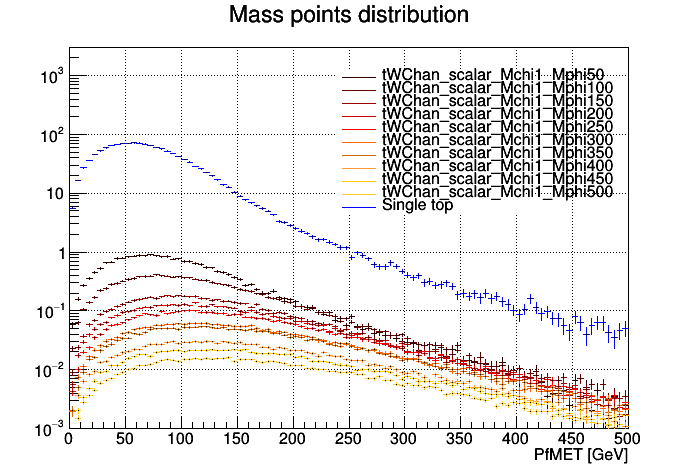
\includegraphics[width=5.2cm, height=3.5cm]{figs/singleTopScalarMET.png}
\end{center}
\end{minipage}
\begin{minipage}[b]{.02\textwidth}\end{minipage}
\begin{minipage}[b]{.49\textwidth}
\vspace{-5pt}
\begin{block}{\centering Pseudoscalar}\end{block}
\begin{center}
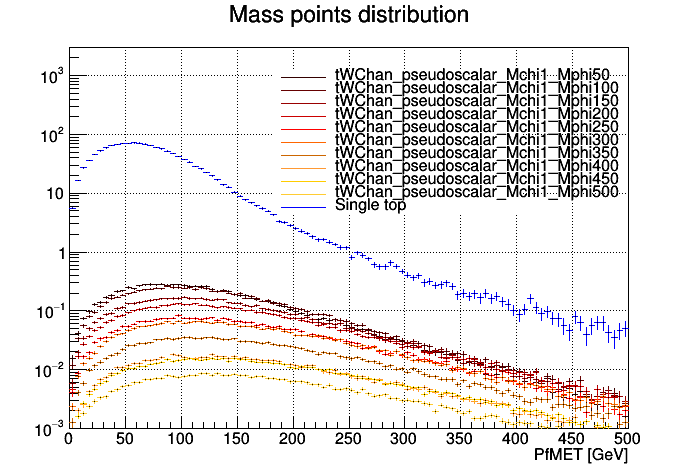
\includegraphics[width=5.2cm, height=3.5cm]{figs/singleTopPseudoMET.png}
\end{center}
\end{minipage}
\end{figure} \vfill

\vspace{-5pt}
\begin{block}{\centering $t \bar t$+DM}\end{block} \vspace{-10pt}
\begin{figure}[htbp]
\centering
\begin{minipage}[b]{.49\textwidth}
\begin{center}
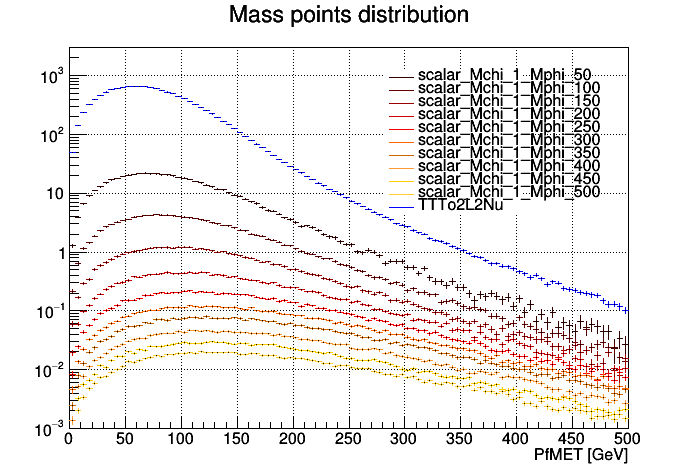
\includegraphics[width=5.2cm, height=3.5cm]{figs/scalarMETmChi1.png}
\end{center}
\end{minipage}\hfill
\begin{minipage}[b]{.49\textwidth}
\begin{center}
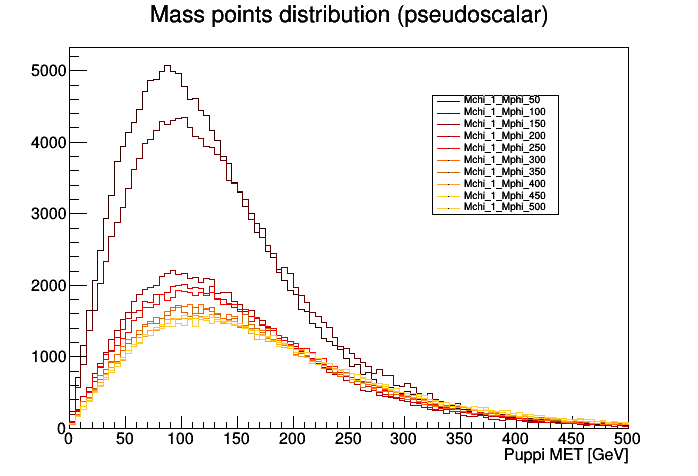
\includegraphics[width=5.2cm, height=3.5cm]{figs/pseudoscalarMETmChi1.png}
\end{center}
\end{minipage} \hfill
\end{figure} \vfill
\end{frame}

\begin{frame}{Objects definition I}
\justifying
%We are currently using the following objects: \vfill

\vspace{5pt} \begin{block}{\centering Triggers}\end{block} \vspace{-6pt}
\begin{itemize}
\justifying
\item \alert{Single and double lepton triggers} combined to gain statistics, and any possible double counting of events in multiple trigger is taken care of;
\item Trigger and lepton $p_T$ carefully chosen to avoid any turn-on effect;
\item SingleMuon, SingleEle, DoubleMuon, DoubleEG, MuonEG (2016) and SingleMuon, EGamma, DoubleMuon, MuonEG (2017/2018) data streams considered;
\item All the triggers used and their efficiencies (computed using orthogonal MET datasets) are listed in the backup.
\end{itemize} \vfill

\begin{block}{\centering Leptons}\end{block} \vspace{-6pt}
\begin{itemize}
\justifying
\item Analysis relies on the \textbf{selection of events with two leptons}, with a leading (trailing) $p_T >$ 25 (20) GeV and $|\eta| < 2.4$;
\item \alert{Medium cut based POG WP used for electrons} without additional isolation cut;
\item \alert{Medium cut based POG WP for muons} with tight isolation (pfRelIso04\_all $< 0.15$);
\item Additional small cuts on the impact parameters to reduce the non-prompt contamination in the ptmiss tail ($|d_0| < 0.05$ cm, $|d_z| < 0.1$ cm, $S_{3D}^d < 4$).
\end{itemize}
\end{frame}

\begin{frame}{Objects definition II}
\justifying
\vspace{5pt} \begin{block}{\centering Jets}\end{block}
\begin{itemize}
\justifying
\item Clustered from the PF candidates using the \textbf{anti-kT algorithm};
\item Basic selection: $p_T > 30$ GeV, $|\eta| < 2.4$;
\item \alert{Tight JET/MET POG working point} (efficiency and background rejection $>$ 98\%), \textbf{tight jet PU ID} applied to jets with $p_T < 50$ GeV to reject PU jets contamination;
\item $\Delta R > 0.4$ away from any lepton passing the criteria established for analysis to prevent signal leptons clustered as jets from entering the jet counting.
\end{itemize} \vfill

\vspace{5pt}
\begin{block}{\centering B-tag}\end{block}
\begin{itemize}
\justifying
\item B-Tagging and Vertexing POG \alert{deep CSV b-tag medium working point} (high efficiency, misidentification rate for a light jet as a b-jet $\sim 1\%$).
%\item B-tagging weight larger than 0.6321, 0.4941 or 0.4184 (2016, 2017 or 2018).
\end{itemize} \vfill

\vspace{5pt}
\begin{block}{\centering Missing transverse momentum}\end{block}
\begin{itemize}
\justifying
\item \alert{PfType1MET} considered by propagating the JECs to the ptmiss;
\item All \textbf{recommended filters applied} to filter anomalous high ptmiss events due to several detector issues, such as eventual dead cells in the calorimeters;
\item XY-shift ($\phi$ modulation fix) and EE noise (2017) corrections applied on top.
\end{itemize} \vfill
\end{frame}



































\begin{frame}[standout]
Event selection
\end{frame}

\begin{frame}{Event selection}
\justifying
\vspace{5pt}
\begin{block}{\centering Minimal event selection}\end{block} \vfill
\vspace{-5pt}

We require for the analysis at least:
\begin{itemize}
\item Two opposite sign leptons, with leading (trailing) $p_T >$ 25 (20) GeV;
\item Third lepton veto ($p_T < 10$ GeV);
\item A dilepton invariant mass $m_{ll} > 20$ GeV to avoid low mass resonances;
\item At least 1 jet.
\end{itemize} \vfill

\vspace{5pt}
\begin{block}{\centering Pre-selection region}\end{block} \vfill
\vspace{-5pt}

A pre-selection region is then defined by additionally asking for:
\begin{itemize}
\item At least 1 medium deep CSV b-jet;
\item A 76-106 GeV Z-veto on the $ee$ and $\mu \mu$ channels;
\item ptmiss $>$ 100 GeV and stransverse mass $M_{T2}^{ll} >$ 80 GeV to keep this region orthogonal to the $t \bar t$ control regions used by the semileptonic channel.
\end{itemize} \vfill

This region is used as the \alert{basis for the definition of our signals regions}. \vfill
\end{frame}

\begin{frame}{Minimal event selection region}
\begin{columns}
%\begin{column}{1.09\textwidth}
%\begin{block}{\centering $ll$ channel}\end{block}
%\end{column}
\end{columns} \vspace{-5pt}
\begin{columns}
		\begin{column}{0.33\textwidth}
			\begin{center}
			\vspace{-8pt}
			\begin{block}{\centering 2016}\end{block}\vspace{10pt}
     			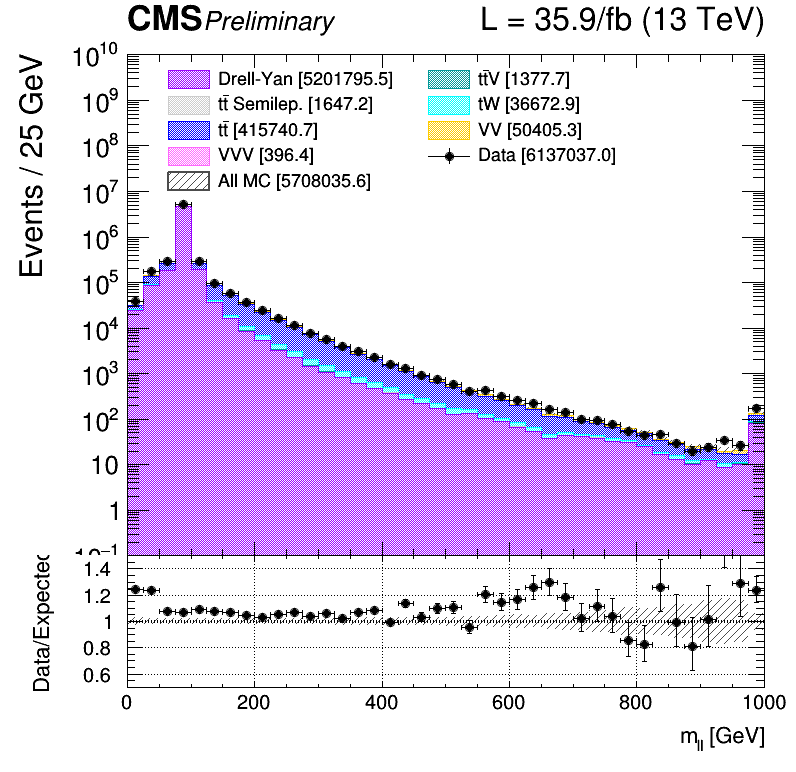
\includegraphics[width=1.0\textwidth, height=100pt]{figs/2016/log_cratio_inclusiveCR_ll_mll.png}
    		\end{center}		
		\end{column} 
		\begin{column}{0.33\textwidth}
			\begin{center}
			\vspace{-8pt}
			\begin{block}{\centering 2017}\end{block}\vspace{10pt}
     			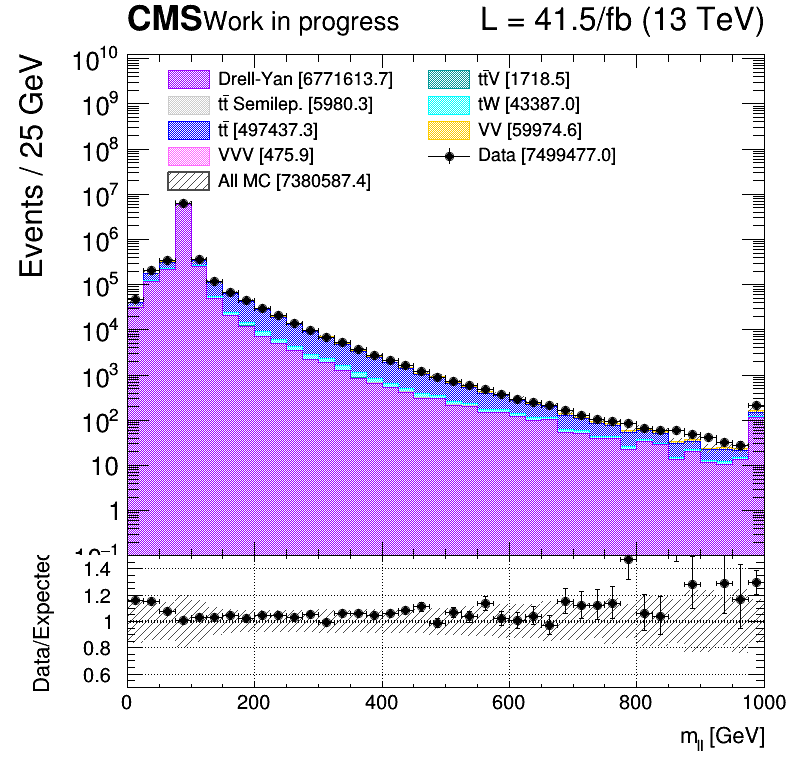
\includegraphics[width=1.0\textwidth, height=100pt]{figs/2017/log_cratio_inclusiveCR_ll_mll.png}
    		\end{center}		
		\end{column} 
		\begin{column}{0.33\textwidth}
			\begin{center}
			\vspace{-8pt}
			\begin{block}{\centering 2018}\end{block}\vspace{10pt}
     			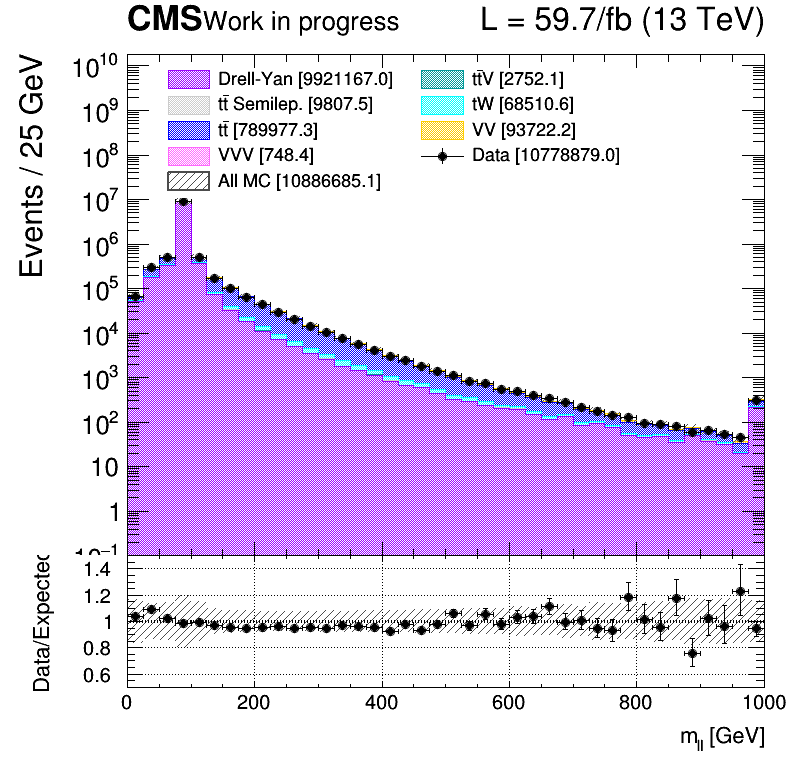
\includegraphics[width=1.0\textwidth, height=100pt]{figs/2018/log_cratio_inclusiveCR_ll_mll.png}
    		\end{center}		
		\end{column}
\end{columns}
\vspace{-5pt}
\begin{columns}
		\begin{column}{0.33\textwidth}
			\begin{center}
				%\begin{block}{\centering Puppi MET}\end{block}	
     			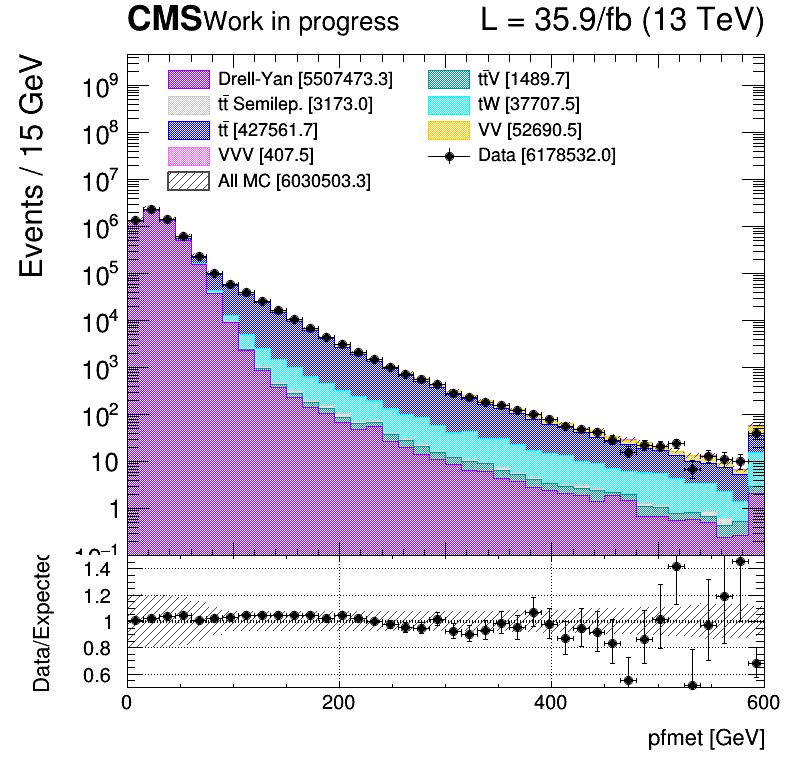
\includegraphics[width=1.0\textwidth, height=100pt]{figs/2016/log_cratio_inclusiveCR_ll_METcorrected_pt.png}
    		\end{center}		
		\end{column}
		\begin{column}{0.33\textwidth}
			\begin{center}
				%\begin{block}{\centering njet}\end{block}	
     			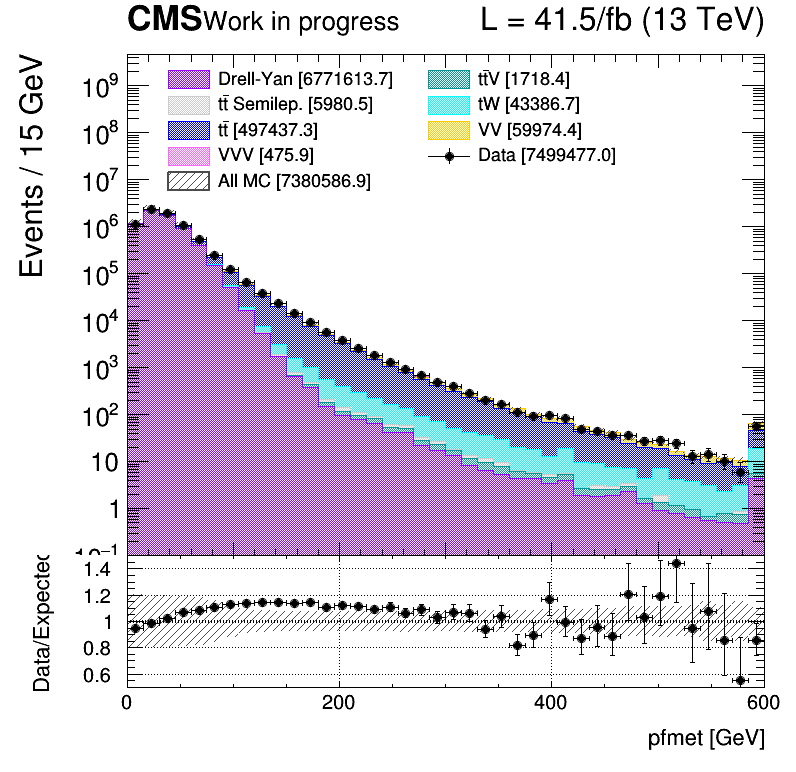
\includegraphics[width=1.0\textwidth, height=100pt]{figs/2017/log_cratio_inclusiveCR_ll_METcorrected_pt.png}
    		\end{center}		
		\end{column}
		\begin{column}{0.33\textwidth}
			\begin{center}
				%\begin{block}{\centering nbjet}\end{block}	
     			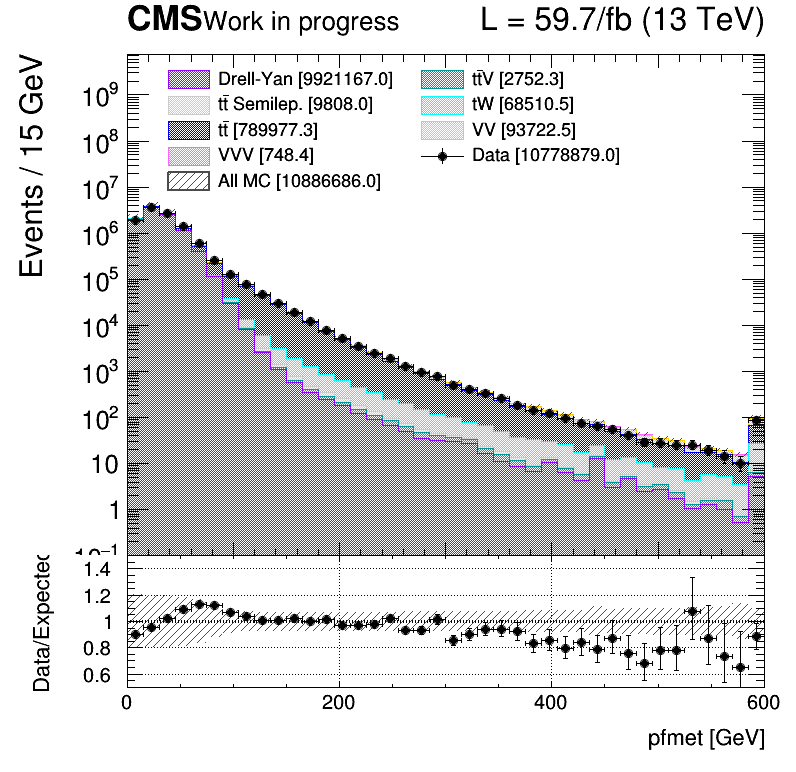
\includegraphics[width=1.0\textwidth, height=100pt]{figs/2018/log_cratio_inclusiveCR_ll_METcorrected_pt.png}
    		\end{center}		
		\end{column}
\end{columns} \vfill
\end{frame}

\begin{frame}{Pre-selection region}
\begin{columns}
%\begin{column}{1.09\textwidth}
%\begin{block}{\centering $ll$ channel}\end{block}
%\end{column}
\end{columns} \vspace{-5pt}
\begin{columns}
		\begin{column}{0.33\textwidth}
			\begin{center}
			\vspace{-8pt}
			\begin{block}{\centering 2016}\end{block}\vspace{10pt}
     			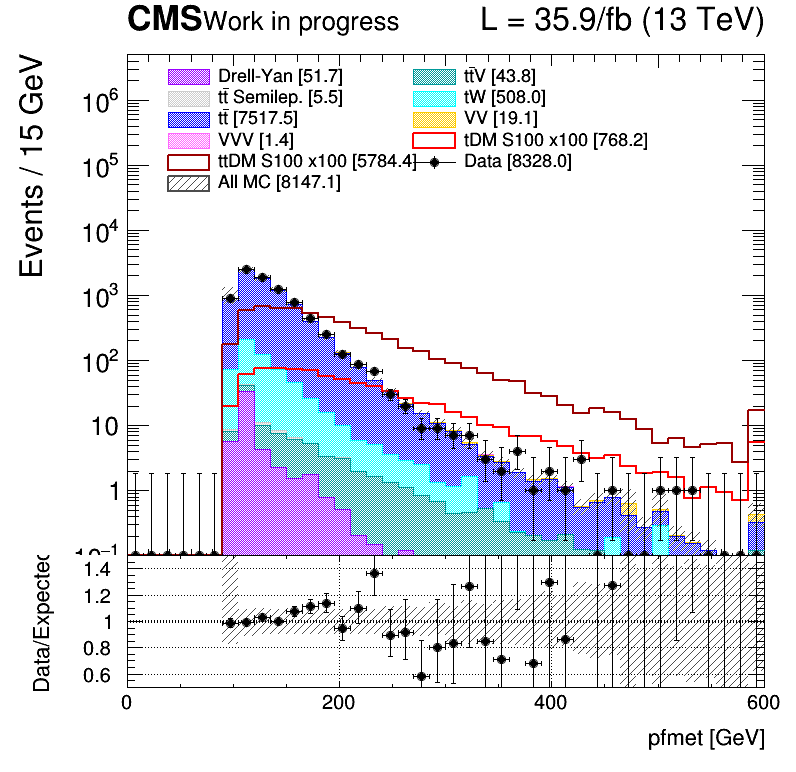
\includegraphics[width=1.0\textwidth, height=100pt]{figs/2016/SmearSR-ttDM-scalar100/log_cratio_topCR_ll_METcorrected_pt.png}
    		\end{center}		
		\end{column} 
		\begin{column}{0.33\textwidth}
			\begin{center}
			\vspace{-8pt}
			\begin{block}{\centering 2017}\end{block}\vspace{10pt}
     			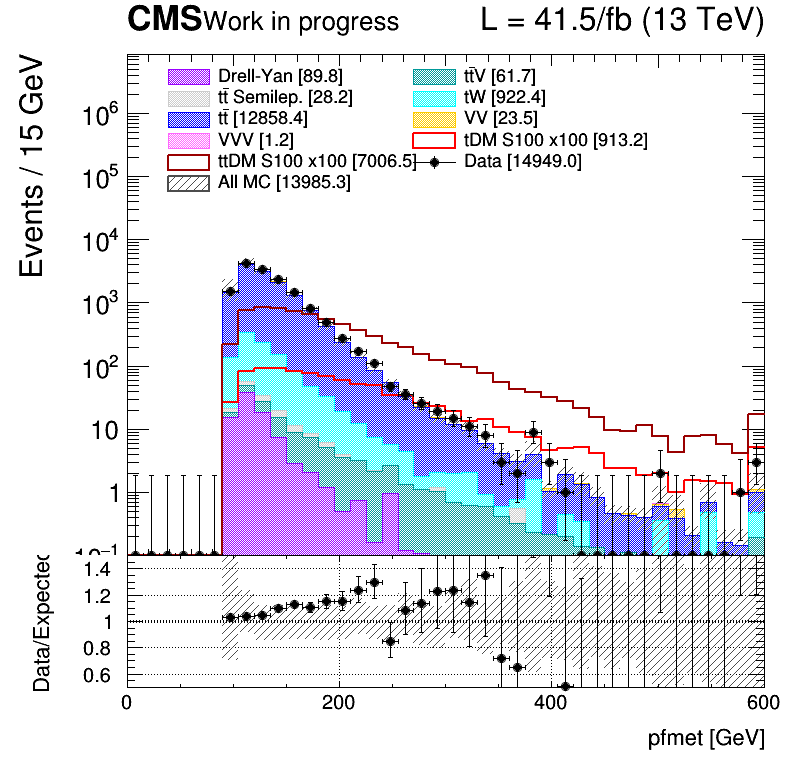
\includegraphics[width=1.0\textwidth, height=100pt]{figs/2017/SmearSR-ttDM-scalar100/log_cratio_topCR_ll_METcorrected_pt.png}
    		\end{center}		
		\end{column} 
		\begin{column}{0.33\textwidth}
			\begin{center}
			\vspace{-8pt}
			\begin{block}{\centering 2018}\end{block}\vspace{10pt}
     			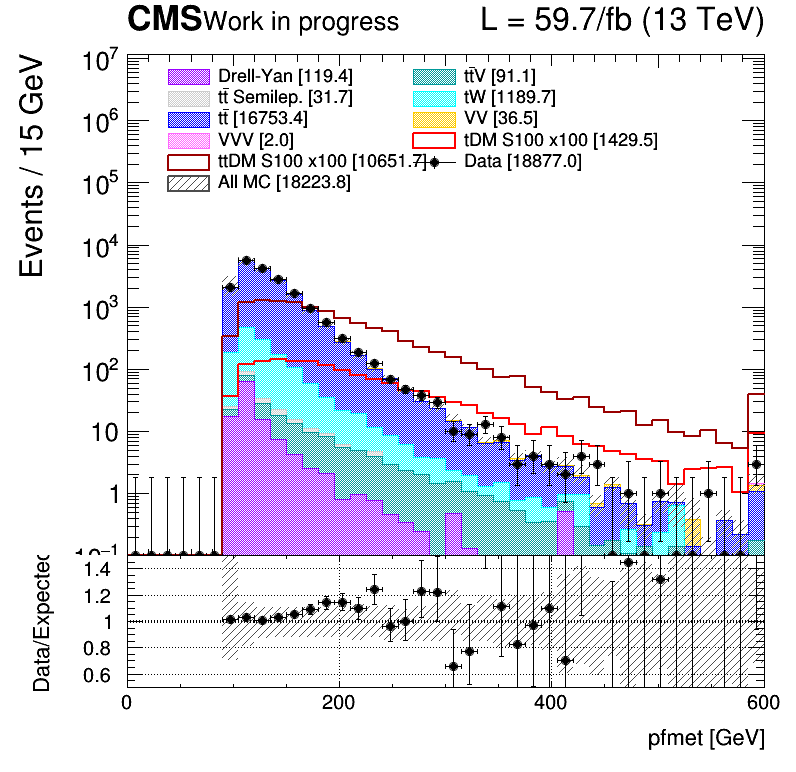
\includegraphics[width=1.0\textwidth, height=100pt]{figs/2018/SmearSR-ttDM-scalar100/log_cratio_topCR_ll_METcorrected_pt.png}
    		\end{center}		
		\end{column}
\end{columns}
\vspace{-5pt}
\begin{columns}
		\begin{column}{0.33\textwidth}
			\begin{center}
				%\begin{block}{\centering Puppi MET}\end{block}	
     			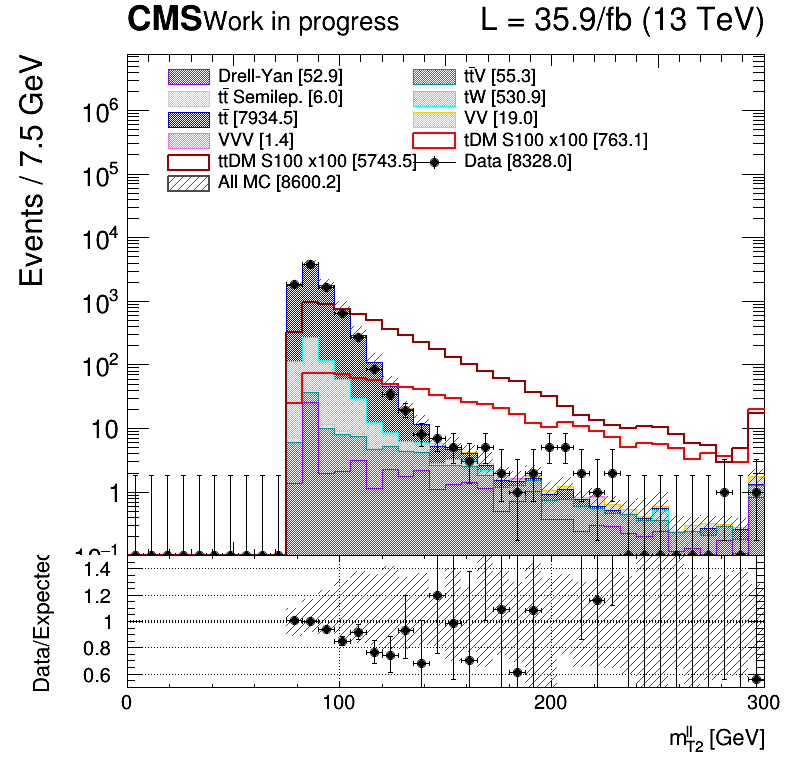
\includegraphics[width=1.0\textwidth, height=100pt]{figs/2016/SmearSR-ttDM-scalar100/log_cratio_topCR_ll_mt2ll.png}
    		\end{center}		
		\end{column}
		\begin{column}{0.33\textwidth}
			\begin{center}
				%\begin{block}{\centering njet}\end{block}	
     			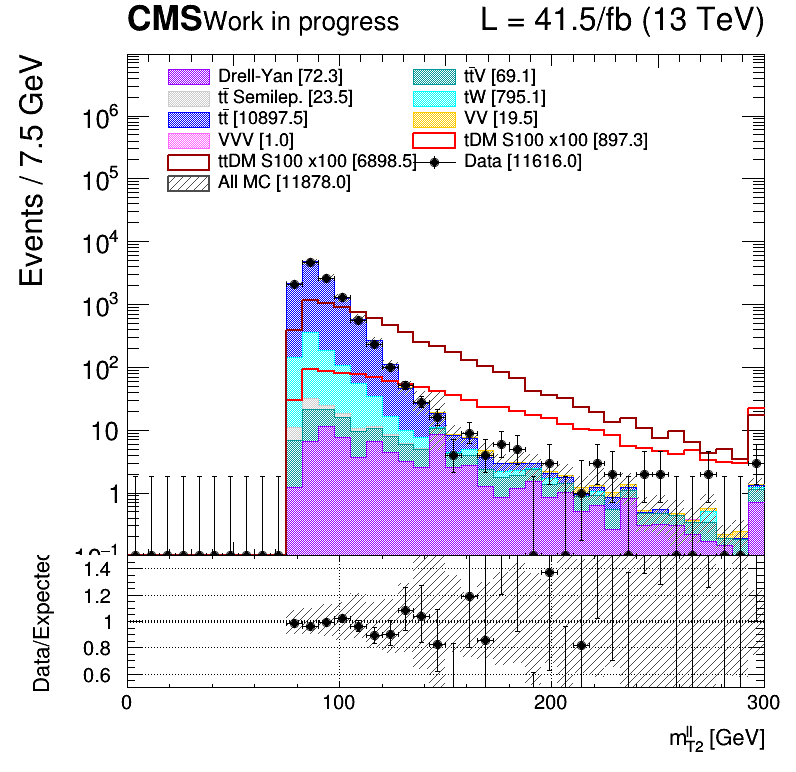
\includegraphics[width=1.0\textwidth, height=100pt]{figs/2017/SmearSR-ttDM-scalar100/log_cratio_topCR_ll_mt2ll.png}
    		\end{center}		
		\end{column}
		\begin{column}{0.33\textwidth}
			\begin{center}
				%\begin{block}{\centering nbjet}\end{block}	
     			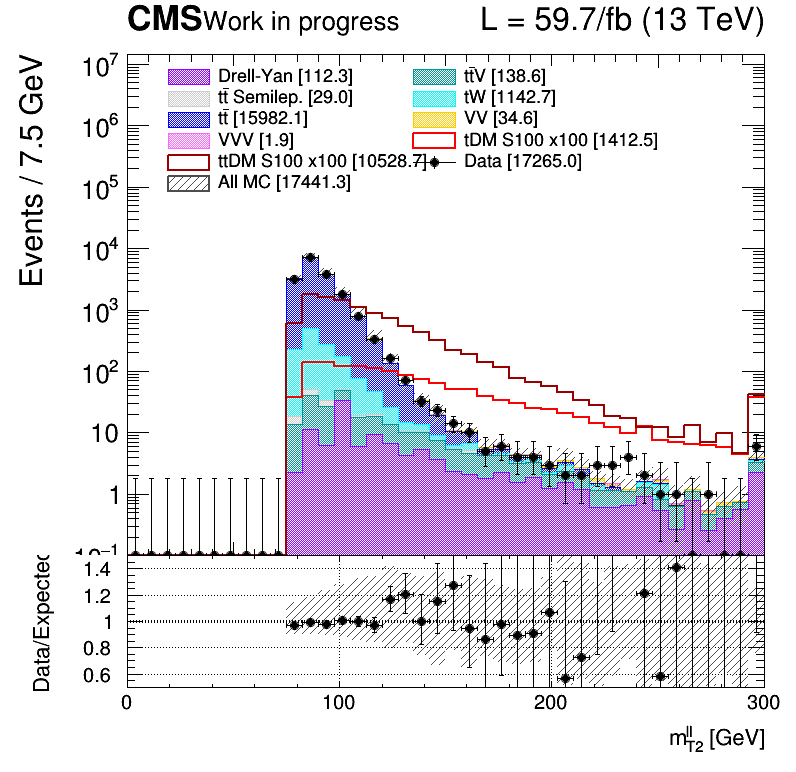
\includegraphics[width=1.0\textwidth, height=100pt]{figs/2018/SmearSR-ttDM-scalar100/log_cratio_topCR_ll_mt2ll.png}
    		\end{center}		
		\end{column}
\end{columns} \vfill
\end{frame}









\begin{frame}[standout]
Background prediction methods
\end{frame}

\begin{frame}{Main background processes}
\justifying
The backgrounds are predicted either directly from \alert{Monte-Carlo simulations or from semi data-driven methods}.

\begin{itemize}
\justifying
\item The \textbf{$\bm{t \bar t}$ and the single top} are taken from simulation accounting for all the variations in the generation parameters;
\item The \textbf{Drell-Yan} yields are obtained from a semi data-driven method using the excluded same flavor region on the Z peak as control region;
\item The \textbf{ttV, diboson, triboson processes and other minor backgrounds} are all taken directly from MC simulations.
\end{itemize} \vfill

Several parameters (QCD scale, PDF variation,...) are varied and included as a systematic (see later), and \textbf{recommended correction factors} (L1 ECAL prefiring in 2016 and 2017, HEM issue in 2018) are also applied to the simulation. \vfill 

\textbf{Several data validation regions} enriched in top and Drell-Yan have been explored to ensure the quality of the prediction made.\vfill
\end{frame}

\begin{frame}{Top control region}
\justifying
Same as the pre-selection region but with ptmiss $> 50$ GeV and $60 < M_{T2}^{ll} < 80$ GeV. \vfill

\begin{columns}
		\begin{column}{0.33\textwidth}
			\begin{center}
			\vspace{-8pt}
			\begin{block}{\centering 2016}\end{block}\vspace{5pt}
     			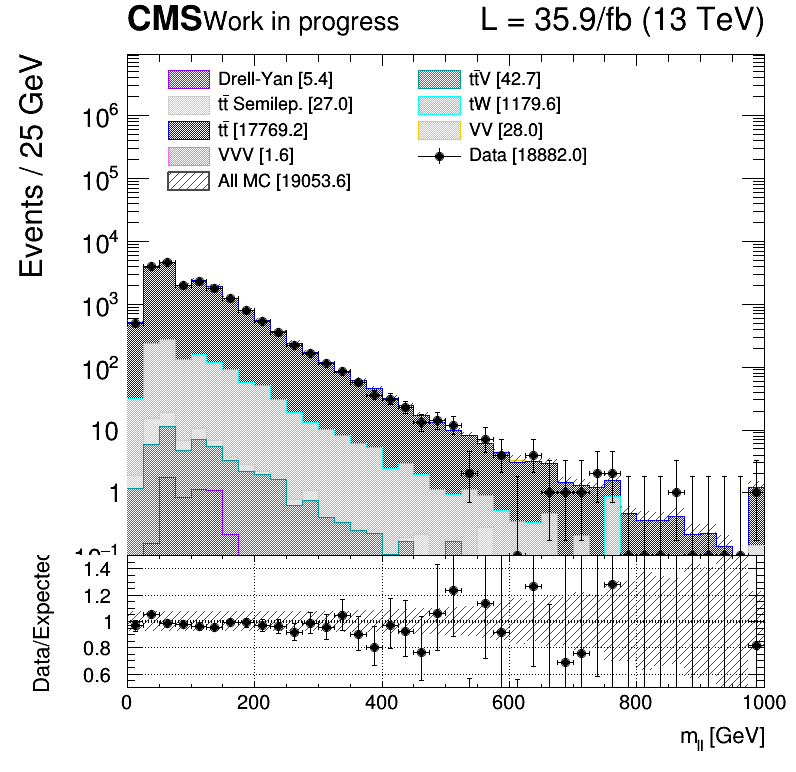
\includegraphics[width=1.0\textwidth, height=95pt]{figs/2016/log_cratio_ttbarCR_ll_mll.png}
    		\end{center}		
		\end{column} 
		\begin{column}{0.33\textwidth}
			\begin{center}
			\vspace{-8pt}
			\begin{block}{\centering 2017}\end{block}\vspace{5pt}
     			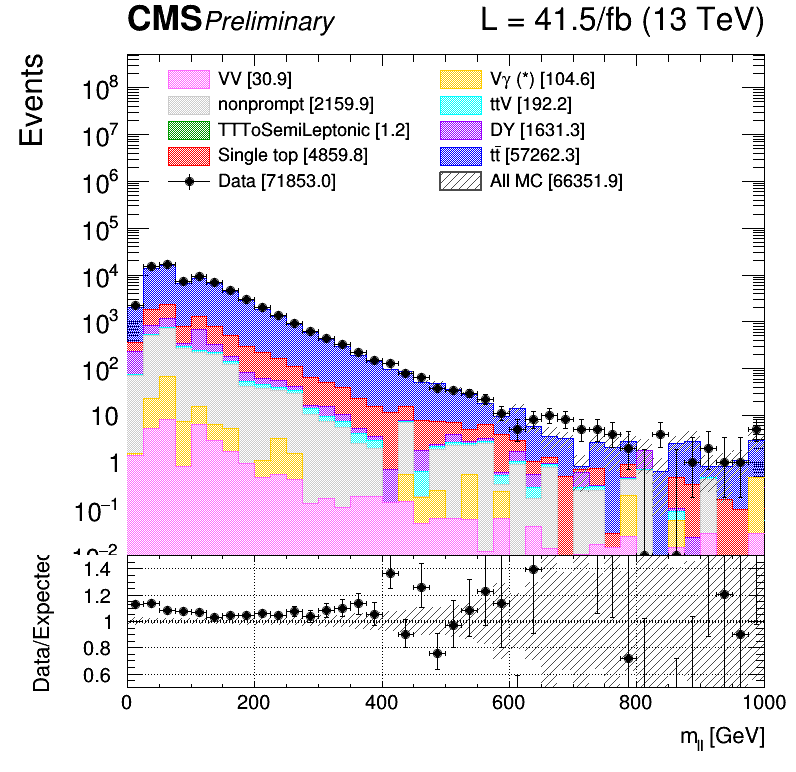
\includegraphics[width=1.0\textwidth, height=95pt]{figs/2017/log_cratio_ttbarCR_ll_mll.png}
    		\end{center}		
		\end{column} 
		\begin{column}{0.33\textwidth}
			\begin{center}
			\vspace{-8pt}
			\begin{block}{\centering 2018}\end{block}\vspace{5pt}
     			\includegraphics[width=1.0\textwidth, height=95pt]{figs/2018/log_cratio_ttbarCR_ll_mll.png}
    		\end{center}		
		\end{column}
\end{columns}

\vspace{-5pt}
\begin{columns}
		\begin{column}{0.33\textwidth}
			\begin{center}
				%\begin{block}{\centering Puppi MET}\end{block}	
     			\includegraphics[width=1.0\textwidth, height=95pt]{figs/2016/log_cratio_ttbarCR_ll_METcorrected_pt.png}
    		\end{center}		
		\end{column}
		\begin{column}{0.33\textwidth}
			\begin{center}
				%\begin{block}{\centering njet}\end{block}	
     			\includegraphics[width=1.0\textwidth, height=95pt]{figs/2017/log_cratio_ttbarCR_ll_METcorrected_pt.png}
    		\end{center}		
		\end{column}
		\begin{column}{0.33\textwidth}
			\begin{center}
				%\begin{block}{\centering nbjet}\end{block}	
     			\includegraphics[width=1.0\textwidth, height=95pt]{figs/2018/log_cratio_ttbarCR_ll_METcorrected_pt.png}
    		\end{center}		
		\end{column}
\end{columns} \vfill
\end{frame}

\begin{frame}{DY Rin-out method}
\justifying
We want to find a way to \alert{estimate the DY yields outside of the Z-peak from the data}, in the minimal event selection region:

\begin{itemize}
\justifying
\item Given the presence of large backgrounds (such as $t \bar t$) in the analysis region, we go inside of the Z-peak to compute the \textbf{Rin-out factor}:
\begin{equation*}
N^{out}_{DY} = N^{in}_{DY, data} \cdot \kappa \cdot \left (\frac{N^{out}_{DY, MC}}{N^{in}_{DY, MC}} \right ) \equiv N^{in}_{DY, data} \cdot \frac{R_{out/in,\text{ } MC}^{0bj}}{R_{out/in,\text{ } data}^{0bj}} \cdot R_{out/in,\text{ } MC}
\end{equation*}
\item To avoid any bias, the contamination of non-peaking backgrounds is removed and we correct this factor by the ratio $\kappa$ between the data/MC transfer factors in a CR close to the SR (asking for 0 b-jet instead of 1);
\item We then get this Rin-out factor in \textbf{bins of ptmiss and for each channel ($ee$, $\mu \mu$)}:
\end{itemize}

\begin{figure}[htbp]
\begin{center}
\begin{minipage}[b]{.32\textwidth}
\includegraphics[width=4cm, height=3cm]{figs/Rinout2016_data.png}
\end{minipage} \hfill
\begin{minipage}[b]{.32\textwidth}
\includegraphics[width=4cm, height=3cm]{figs/Rinout2017_data.png}
\end{minipage} \hfill
\begin{minipage}[b]{.32\textwidth}
\includegraphics[width=4cm, height=3cm]{figs/Rinout2018_data.png}
\end{minipage} \hfill
\end{center}
\end{figure} \vfill

\vspace{-5pt}
A flat scale factor and a fixed 20\% systematic uncertainty is then applied to the DY. \vfill
\end{frame}

\begin{frame}{DY control region}
\justifying
Same as the pre-selection region but with ptmiss $>$ 30 GeV and Z-veto reversed.
\begin{columns}
		\begin{column}{0.33\textwidth}
			\begin{center}
			\vspace{-8pt}
			\begin{block}{\centering 2016}\end{block}\vspace{5pt}
     			\includegraphics[width=1.0\textwidth, height=95pt]{figs/2016/log_cratio_dyCR_ll_mllpeak.png}
    		\end{center}		
		\end{column} 
		\begin{column}{0.33\textwidth}
			\begin{center}
			\vspace{-8pt}
			\begin{block}{\centering 2017}\end{block}\vspace{5pt}
     			\includegraphics[width=1.0\textwidth, height=95pt]{figs/2017/log_cratio_dyCR_ll_mllpeak.png}
    		\end{center}		
		\end{column} 
		\begin{column}{0.33\textwidth}
			\begin{center}
			\vspace{-8pt}
			\begin{block}{\centering 2018}\end{block}\vspace{5pt}
     			\includegraphics[width=1.0\textwidth, height=95pt]{figs/2018/log_cratio_dyCR_ll_mllpeak.png}
    		\end{center}		
		\end{column}
\end{columns}
\vspace{-5pt}
\begin{columns}
		\begin{column}{0.33\textwidth}
			\begin{center}
				%\begin{block}{\centering Puppi MET}\end{block}	
     			\includegraphics[width=1.0\textwidth, height=95pt]{figs/2016/log_cratio_dyCR_ll_METcorrected_pt.png}
    		\end{center}		
		\end{column}
		\begin{column}{0.33\textwidth}
			\begin{center}
				%\begin{block}{\centering njet}\end{block}	
     			\includegraphics[width=1.0\textwidth, height=95pt]{figs/2017/log_cratio_dyCR_ll_METcorrected_pt.png}
    		\end{center}		
		\end{column}
		\begin{column}{0.33\textwidth}
			\begin{center}
				%\begin{block}{\centering nbjet}\end{block}	
     			\includegraphics[width=1.0\textwidth, height=95pt]{figs/2018/log_cratio_dyCR_ll_METcorrected_pt.png}
    		\end{center}		
		\end{column}
\end{columns} \vfill

%The 0-bjet correction allows us to fix the data/MC discrepancies observed. A large systematic uncertainty is associated to this background, minor in the signal regions. \vfill
\end{frame}












\begin{frame}[standout]
Signal extraction
\end{frame}

\begin{frame}{Global strategy}
\justifying
In this analysis, \alert{two different signal regions} have been used, targeting each one of our signals of interest and each based on the pre-selection region:
\begin{itemize}
\item One \textbf{targeting the $\bm{t/\bar t}$+DM signal}, by considering events having exactly 1 jet, or exactly 2 jets and 1 b-jet;
\item Another one \textbf{targeting the $\bm{t \bar t}$+DM signal}, by considering events having exactly 2 jets and more than 1 b-jet, or more than 2 jets.
\end{itemize} \vfill

\alert{Several different discriminating variables} (ptmiss, stranverse mass $M_{T2}^{ll}$, spin correlated variables, etc.) have been considered. \vfill

Many of such variables require knowledge of the top quark and anti-quark 4-momenta, only available after a \textbf{complete reconstruction of the $t \bar t$ system}, performed whenever possible (details in the backup). \vfill

A \alert{BDT combines the discriminating power} of all the variables considered, and an \textbf{ANN is being used as a cross check}. A complete optimization was followed in order to select the features which maximize the performance. \vfill
\end{frame}

\begin{frame}{Discriminating variables I}
\justifying
\alert{Several discriminating variables} (all detailed in the backup) are considered, such as:
\begin{itemize}
\item The stransverse mass $M_{T2}^{ll}$ and missing transverse momentum;
\item The number of b-jets (only in the $t \bar t$+DM signal region) and $m_{bl}^t$ variable, useful to separate our two signals;
\item Several spin correlated variables, such as $\xi = \cos(\theta_l) \cos(\theta_{\bar l})$ and $c_{\text{hel}}$;
\item $r_{2l}$ and $r_{2l4j}$, defined as the ratio between the $p_{\rm T}^{\rm miss}$ and the $p_T$ of the leptons (plus the 4 first eventual jets for $r_{2l4j}$);
\item The dark $p_T$ and overlapping factor naturally arising from the top reconstruction;
\item Other variables, such as the angle $\Delta \phi$ between the $p_{\rm T}^{\rm miss}$ and the two leptons, and total transverse mass \textit{massT}.
\end{itemize} \vfill

\vspace{10pt}
\begin{table}
\begin{center}
\resizebox{0.6\textwidth}{!}{
\begin{tabular}{ c|c|c|c|c } 
 \hline
 & \multicolumn{2}{c}{\textbf{$t/\bar t$+DM region}} & \multicolumn{2}{c}{\textbf{$t \bar t$+DM region}} \\
 Rank & Variable & Importance & Variable & Importance \\
 \hline
 1 & $M_{T2}^{ll}$ & $5.96 \cdot 10^{-1}$ & $M_{T2}^{ll}$ & $5.87 \cdot 10^{-1}$ \\
 2 & $E_{T}^{\text{miss}}$ & $5.32 \cdot 10^{-1}$ & $E_{T}^{\text{miss}}$ & $5.09 \cdot 10^{-1}$ \\
 3 & massT & $3.11 \cdot 10^{-1}$ & massT & $3.98 \cdot 10^{-1}$ \\ 
 4 & $r2l4j$ & $1.70 \cdot 10^{-1}$ & $r2l4j$ & $3.45 \cdot 10^{-1}$ \\ 
 5 & $m_{bl}^t$ & $7.05 \cdot 10^{-2}$ & $m_{bl}^t$ & $1.72 \cdot 10^{-1}$ \\
 6 & $r2l$ & $2.63 \cdot 10^{-2}$ & Dark $p_T$ & $3.92 \cdot 10^{-2}$ \\
\hline
\end{tabular}
}
\caption{Ranking of importance of the main variables for the scalar 500 GeV case.}
\end{center}
\end{table} \vfill	
\end{frame}


\begin{frame}{Discriminating variables II}
\begin{columns}
\begin{column}{1.09\textwidth}
\begin{block}{\centering 2016, pre-selection region}\end{block} \vspace{5pt}
\end{column}
\end{columns} \vspace{-5pt}
\begin{columns}
		\begin{column}{0.33\textwidth}
			\begin{center}
     			\includegraphics[width=1.0\textwidth, height=105pt]{figs/2016/SmearSR-ttDM-scalar100/log_cratio_topCR_ll_mt2ll.png}
    		\end{center}		
		\end{column} 
		\begin{column}{0.33\textwidth}
			\begin{center}
     			\includegraphics[width=1.0\textwidth, height=105pt]{figs/2016/SmearSR-ttDM-scalar100/log_cratio_topCR_ll_METcorrected_pt.png}
    		\end{center}		
		\end{column} 
		\begin{column}{0.33\textwidth}
			\begin{center}
     			\includegraphics[width=1.0\textwidth, height=105pt]{figs/2016/SmearSR-ttDM-scalar100/log_cratio_topCR_ll_massT.png}
    		\end{center}		
		\end{column}
\end{columns}
\vspace{-5pt}
\begin{columns}
		\begin{column}{0.33\textwidth}
			\begin{center}
				%\begin{block}{\centering Puppi MET}\end{block}	
     			\includegraphics[width=1.0\textwidth, height=105pt]{figs/2016/SmearSR-ttDM-scalar100/log_cratio_topCR_ll_r2l4j.png}
    		\end{center}		
		\end{column}
		\begin{column}{0.33\textwidth}
			\begin{center}
				%\begin{block}{\centering njet}\end{block}	
     			\includegraphics[width=1.0\textwidth, height=105pt]{figs/2016/SmearSR-ttDM-scalar100/log_cratio_topCR_ll_mblt.png}
    		\end{center}		
		\end{column}
		\begin{column}{0.33\textwidth}
			\begin{center}
				%\begin{block}{\centering nbjet}\end{block}	
     			\includegraphics[width=1.0\textwidth, height=105pt]{figs/2016/SmearSR-ttDM-scalar100/log_cratio_topCR_ll_dark_pt.png}
    		\end{center}		
		\end{column}
\end{columns} \vfill
\end{frame}

\begin{frame}{Discriminating variables III}
\begin{columns}
\begin{column}{1.09\textwidth}
\begin{block}{\centering 2017, pre-selection region}\end{block} \vspace{5pt}
\end{column}
\end{columns} \vspace{-5pt}
\begin{columns}
		\begin{column}{0.33\textwidth}
			\begin{center}
     			\includegraphics[width=1.0\textwidth, height=105pt]{figs/2017/SmearSR-ttDM-scalar100/log_cratio_topCR_ll_mt2ll.png}
    		\end{center}		
		\end{column} 
		\begin{column}{0.33\textwidth}
			\begin{center}
     			\includegraphics[width=1.0\textwidth, height=105pt]{figs/2017/SmearSR-ttDM-scalar100/log_cratio_topCR_ll_METcorrected_pt.png}
    		\end{center}		
		\end{column} 
		\begin{column}{0.33\textwidth}
			\begin{center}
     			\includegraphics[width=1.0\textwidth, height=105pt]{figs/2017/SmearSR-ttDM-scalar100/log_cratio_topCR_ll_massT.png}
    		\end{center}		
		\end{column}
\end{columns}
\vspace{-5pt}
\begin{columns}
		\begin{column}{0.33\textwidth}
			\begin{center}
				%\begin{block}{\centering Puppi MET}\end{block}	
     			\includegraphics[width=1.0\textwidth, height=105pt]{figs/2017/SmearSR-ttDM-scalar100/log_cratio_topCR_ll_r2l4j.png}
    		\end{center}		
		\end{column}
		\begin{column}{0.33\textwidth}
			\begin{center}
				%\begin{block}{\centering njet}\end{block}	
     			\includegraphics[width=1.0\textwidth, height=105pt]{figs/2017/SmearSR-ttDM-scalar100/log_cratio_topCR_ll_mblt.png}
    		\end{center}		
		\end{column}
		\begin{column}{0.33\textwidth}
			\begin{center}
				%\begin{block}{\centering nbjet}\end{block}	
     			\includegraphics[width=1.0\textwidth, height=105pt]{figs/2017/SmearSR-ttDM-scalar100/log_cratio_topCR_ll_dark_pt.png}
    		\end{center}		
		\end{column}
\end{columns} \vfill
\end{frame}

\begin{frame}{Discriminating variables IV}
\begin{columns}
\begin{column}{1.09\textwidth}
\begin{block}{\centering 2018, pre-selection region}\end{block} \vspace{5pt}
\end{column}
\end{columns} \vspace{-5pt}
\begin{columns}
		\begin{column}{0.33\textwidth}
			\begin{center}
     			\includegraphics[width=1.0\textwidth, height=105pt]{figs/2018/SmearSR-ttDM-scalar100/log_cratio_topCR_ll_mt2ll.png}
    		\end{center}		
		\end{column} 
		\begin{column}{0.33\textwidth}
			\begin{center}
     			\includegraphics[width=1.0\textwidth, height=105pt]{figs/2018/SmearSR-ttDM-scalar100/log_cratio_topCR_ll_METcorrected_pt.png}
    		\end{center}		
		\end{column} 
		\begin{column}{0.33\textwidth}
			\begin{center}
     			\includegraphics[width=1.0\textwidth, height=105pt]{figs/2018/SmearSR-ttDM-scalar100/log_cratio_topCR_ll_massT.png}
    		\end{center}		
		\end{column}
\end{columns}
\vspace{-5pt}
\begin{columns}
		\begin{column}{0.33\textwidth}
			\begin{center}
				%\begin{block}{\centering Puppi MET}\end{block}	
     			\includegraphics[width=1.0\textwidth, height=105pt]{figs/2018/SmearSR-ttDM-scalar100/log_cratio_topCR_ll_r2l4j.png}
    		\end{center}		
		\end{column}
		\begin{column}{0.33\textwidth}
			\begin{center}
				%\begin{block}{\centering njet}\end{block}	
     			\includegraphics[width=1.0\textwidth, height=105pt]{figs/2018/SmearSR-ttDM-scalar100/log_cratio_topCR_ll_mblt.png}
    		\end{center}		
		\end{column}
		\begin{column}{0.33\textwidth}
			\begin{center}
				%\begin{block}{\centering nbjet}\end{block}	
     			\includegraphics[width=1.0\textwidth, height=105pt]{figs/2018/SmearSR-ttDM-scalar100/log_cratio_topCR_ll_dark_pt.png}
    		\end{center}		
		\end{column}
\end{columns} \vfill
\end{frame}

\begin{frame}{MVA training}
\justifying
We \alert{trained both a BDT and an ANN}, featuring the following \textbf{common characteristics}:
\vspace{-5pt}
\begin{itemize}
\justifying
\item Mix of standard model $t \bar t$ and single top as backgrounds, and mix of both $t/\bar t$+DM and $t \bar t$+DM as signals;
\item Only events passing the pre-selection cuts are considered for the training;
\item One specific training performed per signal mass point, and per signal region:
\begin{itemize}
\item One targeting the $t/\bar t$+DM signal, by considering events having exactly 1 jet, or exactly 2 jets and 1 b-jet;
\item Another one targeting the $t \bar t$+DM signal, by considering events having exactly 2 jets and more than 1 b-jet, or more than 2 jets.
\end{itemize}

\item 70\%/30\% train/test splitting used ($\sim 50.000$ training events in total);
\item 14 different discriminating variables used as input.
\end{itemize} \vfill

The \alert{BDT was chosen for the analysis} over the ANN, given that it gave $\sim$10\% better upper limits once optimized. \vfill
The BDT output shape is then used to perform a general \textbf{shape analysis}. \vfill
\end{frame}

\begin{frame}{Hyperparameters optimization}
\justifying
The hyperparameters of the BDT \alert{have all been fully optimized} one by one, trying to: 
\begin{itemize}
\item \textbf{Minimize the error} in the test dataset;
\item \textbf{Maximize the discrimination} obtained;
\item All this while trying to keep the training time reasonable enough.
\end{itemize} \vfill

\begin{columns}
		\begin{column}{0.59\textwidth}
		\begin{table}
\begin{center}
\resizebox{\textwidth}{!}{
\begin{tabular}{ c|c } 
\hline
 BDT parameter & Optimized value \\
 \hline
 Maximum depth & 4 \\
 Minimum samples per leaf & 2\% \\
 Loss function & Quadratic \\
 Boost algorithm & Gradient descent \\
 Shrinkage & 0.3 \\
 Grid points $n_{\text{cut}}$ & 1000 \\
 Number of trees & 250 \\
\hline
\end{tabular}
}
\end{center}
\end{table}
		\end{column} 
		\end{columns} \vfill
		
%The following variables were observed to have the most impact on the final results:
%
%\begin{table}
%\begin{center}
%\resizebox{0.6\textwidth}{!}{
%\begin{tabular}{ c|c|c|c|c } 
% \hline
% & \multicolumn{2}{c}{\textbf{$t/\bar t$+DM region}} & \multicolumn{2}{c}{\textbf{$t \bar t$+DM region}} \\
% Rank & Variable & Importance & Variable & Importance \\
% \hline
% 1 & $M_{T2}^{ll}$ & $4.17 \cdot 10^{-1}$ & $M_{T2}^{ll}$ & $3.92 \cdot 10^{-1}$ \\
% 2 & $E_{T}^{\text{miss}}$ & $3.41 \cdot 10^{-1}$ & $E_{T}^{\text{miss}}$ & $3.14 \cdot 10^{-1}$ \\
% 3 & massT & $1.28 \cdot 10^{-1}$ & massT & $2.28 \cdot 10^{-1}$ \\ 
% 4 & $r2l4j$ & $1.14 \cdot 10^{-1}$ & $r2l4j$ & $1.91 \cdot 10^{-1}$ \\ 
% 5 & $m_{bl}^t$ & $6.12 \cdot 10^{-2}$ & $m_{bl}^t$ & $9.35 \cdot 10^{-2}$ \\
% 6 & Dark $p_T$ & $1.59 \cdot 10^{-2}$ & nbJet & $1.69 \cdot 10^{-2}$ \\
%\hline
%\end{tabular}
%}
%\end{center}
%\end{table} \vfill	
\end{frame}

\begin{frame}{ROC curves}
\justifying
%\begin{block}{\centering Scalar mediators}\end{block} \vspace{-10pt}
\alert{ROC curves have been obtained} for all the different mass points available (50 to 500 GeV), for both scalar (left) and pseudoscalar (right) mediators, in both signal regions. \vfill
\vspace{-5pt}

\begin{figure}[htbp]
\centering
\begin{columns}
\begin{column}{1.09\textwidth}
\begin{block}{\centering $t/\bar t$+DM region}\end{block} \vspace{10pt}
\end{column}
\end{columns} \vspace{-16pt}

\begin{columns}
\begin{column}[b]{.50\textwidth}
\begin{center}
\includegraphics[width=4.2cm, height=3.2cm]{figs/groupedROC_scalar_ST.png}
\end{center}
\end{column} \hfill
\begin{column}[b]{.50\textwidth}
\begin{center}
\includegraphics[width=4.2cm, height=3.2cm]{figs/groupedROC_pseudo_ST.png}
\end{center}
\end{column} \hfill
\end{columns} \vfill
\vspace{-5pt}

\begin{columns}
\begin{column}{1.09\textwidth}
\begin{block}{\centering $t \bar t$+DM region}\end{block} \vspace{10pt}
\end{column}
\end{columns} \vspace{-16pt}

\begin{columns}
\begin{column}[b]{.50\textwidth}
\begin{center}
\includegraphics[width=4.2cm, height=3.2cm]{figs/groupedROC_scalar_TTbar.png}
\end{center}
\end{column} \hfill
\begin{column}[b]{.50\textwidth}
\begin{center}
\includegraphics[width=4.2cm, height=3.2cm]{figs/groupedROC_pseudo_TTbar.png}
\end{center}
\end{column} \hfill
\end{columns} \vfill
\label{fig:ROC2}
\end{figure}
\end{frame}


%\vspace{-5pt}
%\begin{block}{\centering Pseudoscalar mediators}\end{block} \vspace{-10pt}
%\begin{figure}[htbp]
%\centering
%\begin{minipage}[b]{.49\textwidth}
%\begin{center}
%\includegraphics[width=5.2cm, height=3.5cm]{figs/ROC_pseudo100.png}
%\end{center}
%\end{minipage}\hfill
%\begin{minipage}[b]{.49\textwidth}
%\begin{center}
%\includegraphics[width=5.2cm, height=3.5cm]{figs/ROC_pseudo500.png}
%\end{center}
%\end{minipage} \hfill
%\end{figure} \vfill
%\end{frame}

\begin{frame}{Overtraining check ($t/\bar t$+DM region)}
\justifying
\begin{block}{\centering Scalar mediators}\end{block} \vspace{-10pt}
\begin{figure}[htbp]
\centering
\begin{minipage}[b]{.49\textwidth}
\vspace{-5pt}
\begin{block}{\centering 100 GeV}\end{block}
\begin{center}
\includegraphics[width=5.2cm, height=3.5cm]{figs/overtraining_scalar100_ST.png}
\end{center}
\end{minipage}
\begin{minipage}[b]{.02\textwidth}\end{minipage}
\begin{minipage}[b]{.49\textwidth}
\vspace{-5pt}
\begin{block}{\centering 500 GeV}\end{block}
\begin{center}
\includegraphics[width=5.2cm, height=3.5cm]{figs/overtraining_scalar500_ST.png}
\end{center}
\end{minipage}
\end{figure} \vfill

\vspace{-5pt}
\begin{block}{\centering Pseudoscalar mediators}\end{block} \vspace{-10pt}
\begin{figure}[htbp]
\centering
\begin{minipage}[b]{.49\textwidth}
\begin{center}
\includegraphics[width=5.2cm, height=3.5cm]{figs/overtraining_pseudo100_ST.png}
\end{center}
\end{minipage}\hfill
\begin{minipage}[b]{.49\textwidth}
\begin{center}
\includegraphics[width=5.2cm, height=3.5cm]{figs/overtraining_pseudo500_ST.png}
\end{center}
\end{minipage} \hfill
\end{figure} \vfill
\end{frame}

\begin{frame}{Overtraining check ($t \bar t$+DM region)}
\justifying
\begin{block}{\centering Scalar mediators}\end{block} \vspace{-10pt}
\begin{figure}[htbp]
\centering
\begin{minipage}[b]{.49\textwidth}
\vspace{-5pt}
\begin{block}{\centering 100 GeV}\end{block}
\begin{center}
\includegraphics[width=5.2cm, height=3.5cm]{figs/overtraining_scalar100_TTbar.png}
\end{center}
\end{minipage}
\begin{minipage}[b]{.02\textwidth}\end{minipage}
\begin{minipage}[b]{.49\textwidth}
\vspace{-5pt}
\begin{block}{\centering 500 GeV}\end{block}
\begin{center}
\includegraphics[width=5.2cm, height=3.5cm]{figs/overtraining_scalar500_TTbar.png}
\end{center}
\end{minipage}
\end{figure} \vfill

\vspace{-5pt}
\begin{block}{\centering Pseudoscalar mediators}\end{block} \vspace{-10pt}
\begin{figure}[htbp]
\centering
\begin{minipage}[b]{.49\textwidth}
\begin{center}
\includegraphics[width=5.2cm, height=3.5cm]{figs/overtraining_pseudo100_TTbar.png}
\end{center}
\end{minipage}\hfill
\begin{minipage}[b]{.49\textwidth}
\begin{center}
\includegraphics[width=5.2cm, height=3.5cm]{figs/overtraining_pseudo500_TTbar.png}
\end{center}
\end{minipage} \hfill
\end{figure} \vfill
\end{frame}


















































\begin{frame}[standout]
Signal regions
\end{frame}

\begin{frame}{Upper limits extraction}
\justifying
As explained before, in this analysis, \alert{two different signal regions} are being used, targeting each one of our signals of interest and each based on the pre-selection region:
\begin{itemize}
\item One \textbf{targeting the $\bm{t/\bar t}$+DM signal}, by considering events having exactly 1 jet, or exactly 2 jets and 1 b-jet;
\item Another one \textbf{targeting the $\bm{t \bar t}$+DM signal}, by considering events having exactly 2 jets and more than 1 b-jet, or more than 2 jets.
\end{itemize} \vfill

The BDT output shapes for each mass point were obtained in each signal region, and a \textbf{general shape analysis} was then performed using such distributions in order to \alert{extract upper limits on the signal strength} for each model\footnote[frame]{The binning of the BDT was chosen as the one optimizing the upper limits obtained while ensuring to have at least a few events ($> 5$) per bin}. 

Such individual results were \textbf{later combined} in order to obtain the final exclusion limits of this analysis, by either:
\begin{itemize}
\justifying
\item On one hand by considering both signal samples together in each signal region separately, and then combining them;
\item Or on the other hand by considering each signal of interest separately in both signal regions, and then combining them.
\end{itemize} \vfill
\end{frame}

\begin{frame}{BDT scalar 100 GeV output pre-fit shapes}
\begin{columns}
\begin{column}{1.09\textwidth}
\begin{block}{\centering $t/\bar t$+DM signal region}\end{block} \vspace{10pt}
\end{column}
\end{columns} \vspace{-24pt}
\begin{columns}
		\begin{column}{0.33\textwidth}
			\begin{center}
			\begin{block}{\centering 2016}\end{block}	
     			\includegraphics[width=1.0\textwidth, height=100pt]{figs/2016/SmearSR-ttDM-scalar100/log_cratio_ST_topCR_ll_BDT_ttDM100_ST_BDT_output_scalar100_customBinsAttempt7.png}
    		\end{center}		
		\end{column} 
		\begin{column}{0.33\textwidth}
			\begin{center}
			\begin{block}{\centering 2017}\end{block}	
     			\includegraphics[width=1.0\textwidth, height=100pt]{figs/2017/SmearSR-ttDM-scalar100/log_cratio_ST_topCR_ll_BDT_ttDM100_ST_BDT_output_scalar100_customBinsAttempt7.png}
    		\end{center}		
		\end{column} 
		\begin{column}{0.33\textwidth}
			\begin{center}
			\begin{block}{\centering 2018}\end{block}	
     			\includegraphics[width=1.0\textwidth, height=100pt]{figs/2018/SmearSR-ttDM-scalar100/log_cratio_ST_topCR_ll_BDT_ttDM100_ST_BDT_output_scalar100_customBinsAttempt7.png}
    		\end{center}		
		\end{column}
\end{columns}

\vspace{-8pt}
\begin{columns}
\begin{column}{1.09\textwidth}
\begin{block}{\centering $t \bar t$+DM signal region}\end{block} \vspace{10pt}
\end{column}
\end{columns} \vspace{-16pt}
\begin{columns}
		\begin{column}{0.33\textwidth}
			\begin{center}
				%\begin{block}{\centering Puppi MET}\end{block}	
     			\includegraphics[width=1.0\textwidth, height=100pt]{figs/2016/SmearSR-ttDM-scalar100/log_cratio_TTbar_topCR_ll_BDT_ttDM100_TTbar_BDT_output_scalar100_customBinsAttempt7.png}
    		\end{center}		
		\end{column}
		\begin{column}{0.33\textwidth}
			\begin{center}
				%\begin{block}{\centering njet}\end{block}	
     			\includegraphics[width=1.0\textwidth, height=100pt]{figs/2017/SmearSR-ttDM-scalar100/log_cratio_TTbar_topCR_ll_BDT_ttDM100_TTbar_BDT_output_scalar100_customBinsAttempt7.png}
    		\end{center}		
		\end{column}
		\begin{column}{0.33\textwidth}
			\begin{center}
				%\begin{block}{\centering nbjet}\end{block}	
     			\includegraphics[width=1.0\textwidth, height=100pt]{figs/2018/SmearSR-ttDM-scalar100/log_cratio_TTbar_topCR_ll_BDT_ttDM100_TTbar_BDT_output_scalar100_customBinsAttempt7.png}
    		\end{center}		
		\end{column}
\end{columns} \vfill
\end{frame}

\begin{frame}{BDT scalar 500 GeV output pre-fit shapes}
\begin{columns}
\begin{column}{1.09\textwidth}
\begin{block}{\centering $t/\bar t$+DM signal region}\end{block} \vspace{10pt}
\end{column}
\end{columns} \vspace{-24pt}
\begin{columns}
		\begin{column}{0.33\textwidth}
			\begin{center}
			\begin{block}{\centering 2016}\end{block}	
     			\includegraphics[width=1.0\textwidth, height=100pt]{figs/2016/SmearSR-ttDM-scalar500/log_cratio_ST_topCR_ll_BDT_ttDM500_ST_BDT_output_scalar500_customBinsAttempt7.png}
    		\end{center}		
		\end{column} 
		\begin{column}{0.33\textwidth}
			\begin{center}
			\begin{block}{\centering 2017}\end{block}	
     			\includegraphics[width=1.0\textwidth, height=100pt]{figs/2017/SmearSR-ttDM-scalar500/log_cratio_ST_topCR_ll_BDT_ttDM500_ST_BDT_output_scalar500_customBinsAttempt7.png}
    		\end{center}		
		\end{column} 
		\begin{column}{0.33\textwidth}
			\begin{center}
			\begin{block}{\centering 2018}\end{block}	
     			\includegraphics[width=1.0\textwidth, height=100pt]{figs/2018/SmearSR-ttDM-scalar500/log_cratio_ST_topCR_ll_BDT_ttDM500_ST_BDT_output_scalar500_customBinsAttempt7.png}
    		\end{center}		
		\end{column}
\end{columns}

\vspace{-8pt}
\begin{columns}
\begin{column}{1.09\textwidth}
\begin{block}{\centering $t \bar t$+DM signal region}\end{block} \vspace{10pt}
\end{column}
\end{columns} \vspace{-16pt}
\begin{columns}
		\begin{column}{0.33\textwidth}
			\begin{center}
				%\begin{block}{\centering Puppi MET}\end{block}	
     			\includegraphics[width=1.0\textwidth, height=100pt]{figs/2016/SmearSR-ttDM-scalar500/log_cratio_TTbar_topCR_ll_BDT_ttDM500_TTbar_BDT_output_scalar500_customBinsAttempt7.png}
    		\end{center}		
		\end{column}
		\begin{column}{0.33\textwidth}
			\begin{center}
				%\begin{block}{\centering njet}\end{block}	
     			\includegraphics[width=1.0\textwidth, height=100pt]{figs/2017/SmearSR-ttDM-scalar500/log_cratio_TTbar_topCR_ll_BDT_ttDM500_TTbar_BDT_output_scalar500_customBinsAttempt7.png}
    		\end{center}		
		\end{column}
		\begin{column}{0.33\textwidth}
			\begin{center}
				%\begin{block}{\centering nbjet}\end{block}	
     			\includegraphics[width=1.0\textwidth, height=100pt]{figs/2018/SmearSR-ttDM-scalar500/log_cratio_TTbar_topCR_ll_BDT_ttDM500_TTbar_BDT_output_scalar500_customBinsAttempt7.png}
    		\end{center}		
		\end{column}
\end{columns} \vfill
\end{frame}















\begin{frame}[standout]
Systematic uncertainties
\end{frame}

\begin{frame}{Systematic uncertainties}
\justifying
On top of statistical uncertainties, \alert{many systematics uncertainties} have been considered: \vfill

\begin{block}{\centering Theoretical uncertainties}\end{block} 

\begin{itemize}
\justifying
\item PDF and higher order corrections ($\sim$4\%), underlying event (1.5\%) and parton shower modeling ($\sim$4\%), renormalization and factorization scales.
\end{itemize} \vfill

\begin{block}{\centering Experimental uncertainties}\end{block}

\begin{itemize}
\justifying
\item Luminosity ($\sim$2.5\%), pileup modeling ($\sim$5\%), lepton trigger ($\sim$2\%), lepton efficiency and energy scale ($\sim$2\%), jet energy scale ($\sim$3\%), ptmiss mismodelling ($\sim$3\%), b-tagging efficiency, top $p_T$ reweighting, ECAL prefiring.
\end{itemize} \vfill

\begin{block}{\centering Background specific uncertainties}\end{block}

\begin{itemize}
\justifying
\item MC statistical uncertainties;
\item 20\% systematic uncertainty associated to the DY process in order to cover for the non-flatness of the $R_{\text{in-out}}$ transfer factor;
\item 30\% uncertainty associated to the normalization of all the minor backgrounds, except for the ttV, for which a 50\% systematic uncertainty is associated.
\end{itemize} \vfill
\end{frame}

\begin{frame}{Pulls and impact plots}
\justifying
\begin{figure}[htbp]
\centering
\begin{block}{\centering 2016, scalar}\end{block}	\vspace{-8pt}

\begin{minipage}[b]{0.49\textwidth}
\begin{center}
\centering \begin{block}{\centering 100 GeV}\end{block}	
\includegraphics[width=5.1cm, height=4.2cm]{figs/impacts_2016_both_scalar_100.pdf}
\end{center}
\end{minipage}\hfill
\begin{minipage}[b]{0.49\textwidth}
\begin{center}
\centering \begin{block}{\centering 500 GeV}\end{block}	
\includegraphics[width=5.1cm, height=4.2cm]{figs/impacts_2016_both_scalar_500.pdf}
\end{center}
\end{minipage} \hfill
\end{figure}

The most important systematic for most mass points is the normalization of the ttV process. \\
$\rightarrow$ Additional impact plots can be found in the backup. \vfill
\end{frame}

%\begin{frame}{Pulls and impact plots}
%\begin{column}{0.49\textwidth}
%\begin{figure}[htbp]
%\centering
%\begin{minipage}[b]{1.0\textwidth}
%\begin{center}
%\includegraphics[width=12cm, height=10cm]{figs/impacts_2016_both_pseudo_100.pdf}
%\end{center}
%\end{minipage} \hfill
%\begin{minipage}[b]{1.0\textwidth}
%\begin{center}
%\includegraphics[width=12cm, height=10cm]{figs/impacts_2016_both_pseudo_500.pdf}
%\end{center}
%\end{minipage} \hfill
%\label{fig:impactsPseudo2016}
%\end{figure}
%\end{column}
%\end{columns}
%
%\end{frame}








\begin{frame}[standout]
Results obtained
\end{frame}

\begin{frame}{Post-fit plots (scalar 100 GeV)}
\begin{columns}
\begin{column}{1.09\textwidth}
\begin{block}{\centering $t/\bar t$+DM region}\end{block} \vspace{10pt}
\end{column}
\end{columns} \vspace{-24pt}
\begin{columns}
		\begin{column}{0.33\textwidth}
			\begin{center}
			\begin{block}{\centering 2016}\end{block}	
     			\includegraphics[width=1.0\textwidth, height=100pt]{figs/postfits/2016/log_cratio_ST_topCR_ll_BDT_tDM100_TTbar_BDT_output_scalar100_customBinsAttempt7.png}
    		\end{center}		
		\end{column} 
		\begin{column}{0.33\textwidth}
			\begin{center}
			\begin{block}{\centering 2017}\end{block}	
     			\includegraphics[width=1.0\textwidth, height=100pt]{figs/postfits/2017/log_cratio_ST_topCR_ll_BDT_tDM100_TTbar_BDT_output_scalar100_customBinsAttempt7.png}
    		\end{center}		
		\end{column} 
		\begin{column}{0.33\textwidth}
			\begin{center}
			\begin{block}{\centering 2018}\end{block}	
     			\includegraphics[width=1.0\textwidth, height=100pt]{figs/postfits/2018/log_cratio_ST_topCR_ll_BDT_tDM100_TTbar_BDT_output_scalar100_customBinsAttempt7.png}
    		\end{center}		
		\end{column}
\end{columns}

\vspace{-8pt}
\begin{columns}
\begin{column}{1.09\textwidth}
\begin{block}{\centering $t \bar t$+DM region}\end{block} \vspace{10pt}
\end{column}
\end{columns} \vspace{-16pt}
\begin{columns}
		\begin{column}{0.33\textwidth}
			\begin{center}
				%\begin{block}{\centering Puppi MET}\end{block}	
     			\includegraphics[width=1.0\textwidth, height=100pt]{figs/postfits/2016/log_cratio_TTbar_topCR_ll_BDT_ttDM100_TTbar_BDT_output_scalar100_customBinsAttempt7.png}
    		\end{center}		
		\end{column}
		\begin{column}{0.33\textwidth}
			\begin{center}
				%\begin{block}{\centering njet}\end{block}	
     			\includegraphics[width=1.0\textwidth, height=100pt]{figs/postfits/2017/log_cratio_TTbar_topCR_ll_BDT_ttDM100_TTbar_BDT_output_scalar100_customBinsAttempt7.png}
    		\end{center}		
		\end{column}
		\begin{column}{0.33\textwidth}
			\begin{center}
				%\begin{block}{\centering nbjet}\end{block}	
     			\includegraphics[width=1.0\textwidth, height=100pt]{figs/postfits/2018/log_cratio_TTbar_topCR_ll_BDT_ttDM100_TTbar_BDT_output_scalar100_customBinsAttempt7.png}
    		\end{center}		
		\end{column}
\end{columns} \vfill
\end{frame}

\begin{frame}{Post-fit plots (scalar 500 GeV)}
\begin{columns}
\begin{column}{1.09\textwidth}
\begin{block}{\centering $t/\bar t$+DM region}\end{block} \vspace{10pt}
\end{column}
\end{columns} \vspace{-24pt}
\begin{columns}
		\begin{column}{0.33\textwidth}
			\begin{center}
			\begin{block}{\centering 2016}\end{block}	
     			\includegraphics[width=1.0\textwidth, height=100pt]{figs/postfits/2016/log_cratio_ST_topCR_ll_BDT_tDM500_TTbar_BDT_output_scalar500_customBinsAttempt7.png}
    		\end{center}		
		\end{column} 
		\begin{column}{0.33\textwidth}
			\begin{center}
			\begin{block}{\centering 2017}\end{block}	
     			\includegraphics[width=1.0\textwidth, height=100pt]{figs/postfits/2017/log_cratio_ST_topCR_ll_BDT_tDM500_TTbar_BDT_output_scalar500_customBinsAttempt7.png}
    		\end{center}		
		\end{column} 
		\begin{column}{0.33\textwidth}
			\begin{center}
			\begin{block}{\centering 2018}\end{block}	
     			\includegraphics[width=1.0\textwidth, height=100pt]{figs/postfits/2018/log_cratio_ST_topCR_ll_BDT_tDM500_TTbar_BDT_output_scalar500_customBinsAttempt7.png}
    		\end{center}		
		\end{column}
\end{columns}

\vspace{-8pt}
\begin{columns}
\begin{column}{1.09\textwidth}
\begin{block}{\centering $t \bar t$+DM region}\end{block} \vspace{10pt}
\end{column}
\end{columns} \vspace{-16pt}
\begin{columns}
		\begin{column}{0.33\textwidth}
			\begin{center}
				%\begin{block}{\centering Puppi MET}\end{block}	
     			\includegraphics[width=1.0\textwidth, height=100pt]{figs/postfits/2016/log_cratio_TTbar_topCR_ll_BDT_ttDM500_TTbar_BDT_output_scalar500_customBinsAttempt7.png}
    		\end{center}		
		\end{column}
		\begin{column}{0.33\textwidth}
			\begin{center}
				%\begin{block}{\centering njet}\end{block}	
     			\includegraphics[width=1.0\textwidth, height=100pt]{figs/postfits/2017/log_cratio_TTbar_topCR_ll_BDT_ttDM500_TTbar_BDT_output_scalar500_customBinsAttempt7.png}
    		\end{center}		
		\end{column}
		\begin{column}{0.33\textwidth}
			\begin{center}
				%\begin{block}{\centering nbjet}\end{block}	
     			\includegraphics[width=1.0\textwidth, height=100pt]{figs/postfits/2018/log_cratio_TTbar_topCR_ll_BDT_ttDM500_TTbar_BDT_output_scalar500_customBinsAttempt7.png}
    		\end{center}		
		\end{column}
\end{columns} \vfill
\end{frame}

\begin{frame}{Upper limits on the signal regions}
\begin{columns}
\begin{column}{1.09\textwidth}
\begin{block}{\centering Scalar upper limits}\end{block}
\end{column}
\end{columns} \vspace{-5pt}
\begin{columns}
		\begin{column}{0.33\textwidth}
			\begin{center}
			\vspace{-8pt}
			\begin{block}{\centering 2016}\end{block} \vspace{-10pt}
     			\includegraphics[width=1.0\textwidth, height=90pt]{figs/limit_scalar_2016_attempt7.png}
    		\end{center}		
		\end{column} 
		\begin{column}{0.33\textwidth}
			\begin{center}
			\vspace{-8pt}
			\begin{block}{\centering 2017}\end{block} \vspace{-10pt}
     			\includegraphics[width=1.0\textwidth, height=90pt]{figs/limit_scalar_2017_attempt7.png}
    		\end{center}		
		\end{column} 
		\begin{column}{0.33\textwidth}
			\begin{center}
			\vspace{-8pt}
			\begin{block}{\centering 2018}\end{block} \vspace{-10pt}
     			\includegraphics[width=1.0\textwidth, height=90pt]{figs/limit_scalar_2018_attempt7.png}
    		\end{center}		
		\end{column}
\end{columns}

\begin{columns}
\begin{column}{1.09\textwidth}
\begin{block}{\centering Pseudoscalar upper limits}\end{block}
\end{column}
\end{columns} \vspace{-15pt}
\begin{columns}
		\begin{column}{0.33\textwidth}
			\begin{center}
				%\begin{block}{\centering Puppi MET}\end{block}	
     			\includegraphics[width=1.0\textwidth, height=90pt]{figs/limit_pseudo_2016_attempt7.png}
    		\end{center}		
		\end{column}
		\begin{column}{0.33\textwidth}
			\begin{center}
				%\begin{block}{\centering njet}\end{block}	
     			\includegraphics[width=1.0\textwidth, height=90pt]{figs/limit_pseudo_2017_attempt7.png}
    		\end{center}		
		\end{column}
		\begin{column}{0.33\textwidth}
			\begin{center}
				%\begin{block}{\centering nbjet}\end{block}	
     			\includegraphics[width=1.0\textwidth, height=90pt]{figs/limit_pseudo_2018_attempt7.png}
    		\end{center}		
		\end{column}
\end{columns} \vfill
\end{frame}

\begin{frame}{Upper limits on the signal models}
\begin{columns}
\begin{column}{1.09\textwidth}
\begin{block}{\centering Scalar upper limits}\end{block}
\end{column}
\end{columns} \vspace{-5pt}
\begin{columns}
		\begin{column}{0.33\textwidth}
			\begin{center}
			\vspace{-8pt}
			\begin{block}{\centering 2016}\end{block} \vspace{-10pt}
     			\includegraphics[width=1.0\textwidth, height=90pt]{figs/limit_scalar_2016_attempt7_v2.png}
    		\end{center}		
		\end{column} 
		\begin{column}{0.33\textwidth}
			\begin{center}
			\vspace{-8pt}
			\begin{block}{\centering 2017}\end{block} \vspace{-10pt}
     			\includegraphics[width=1.0\textwidth, height=90pt]{figs/limit_scalar_2017_attempt7_v2.png}
    		\end{center}		
		\end{column} 
		\begin{column}{0.33\textwidth}
			\begin{center}
			\vspace{-8pt}
			\begin{block}{\centering 2018}\end{block} \vspace{-10pt}
     			\includegraphics[width=1.0\textwidth, height=90pt]{figs/limit_scalar_2018_attempt7_v2.png}
    		\end{center}		
		\end{column}
\end{columns}

\begin{columns}
\begin{column}{1.09\textwidth}
\begin{block}{\centering Pseudoscalar upper limits}\end{block}
\end{column}
\end{columns} \vspace{-15pt}
\begin{columns}
		\begin{column}{0.33\textwidth}
			\begin{center}
				%\begin{block}{\centering Puppi MET}\end{block}	
     			\includegraphics[width=1.0\textwidth, height=90pt]{figs/limit_pseudo_2016_attempt7_v2.png}
    		\end{center}		
		\end{column}
		\begin{column}{0.33\textwidth}
			\begin{center}
				%\begin{block}{\centering njet}\end{block}	
     			\includegraphics[width=1.0\textwidth, height=90pt]{figs/limit_pseudo_2017_attempt7_v2.png}
    		\end{center}		
		\end{column}
		\begin{column}{0.33\textwidth}
			\begin{center}
				%\begin{block}{\centering nbjet}\end{block}	
     			\includegraphics[width=1.0\textwidth, height=90pt]{figs/limit_pseudo_2018_attempt7_v2.png}
    		\end{center}		
		\end{column}
\end{columns} \vfill
\end{frame}

\begin{frame}{Run II legacy limits}
\justifying
\begin{columns}
	\begin{column}{0.5 \textwidth}
\begin{center}
\begin{block}{\centering Scalar mediators}\end{block} \vspace{-10pt}
\includegraphics[width=5.4cm, height=4.8cm]{figs/limit_scalar.png}
\end{center}
\end{column}
	\begin{column}{0.5 \textwidth}
\begin{figure}[htbp]
\begin{center}
\begin{block}{\centering Pseudoscalar mediators}\end{block} \vspace{-8pt}
\includegraphics[width=5.4cm, height=4.8cm]{figs/limit_pseudo.png}
\end{center}
\end{figure}
	\end{column}
	\end{columns} \vfill
	
After combining the limits obtained for the different years, the following \alert{expected (observed) exclusion have been achieved}:
\begin{itemize}
\item Scalar mediators excluded to 215 (180) GeV;
\item Pseudoscalar mediators excluded up to 250 (220) GeV. 
\end{itemize} \vfill
\end{frame}

\begin{frame}{Conclusions}
\justifying
A search for \alert{dark matter produced in association with either one or two top quarks} has been performed, considering in particular its \textbf{dilepton final state}, and analyzing the \textbf{Run II legacy dataset} collected by the CMS detector at 13 TeV. \vfill

This is the \textbf{first time that such a combination of two signals of interest} is performed considering this particular final state. \vfill

In summary, this search managed to:
\begin{itemize}
\justifying
\item Exclude scalar (pseudoscalar) mediators up to 215 (250) GeV respectively;
\item \textbf{Improve by a factor of 3} the scalar exclusion limits published by the CMS collaboration in 2016 using the $t \bar t$+DM model alone;
\item And \textbf{exclude for the first time pseudoscalar mediators} up to 250 GeV.
\end{itemize} \vfill
\end{frame}

\begin{frame}{Future prospects}
\justifying
Several \alert{additions and improvements could be considered} to improve the results obtained:
\begin{itemize}
\justifying
\item The \textbf{combination of these results} with the semileptonic and hadronic final states will be beneficial given their large branching ratios;
\item The \textbf{continuous operation of the LHC} and future data yet to be collected is expected to improve these results as well;
\item Given the importance of the ttV normalization systematic uncertainty, the definition of a \textbf{dedicated control region} might be beneficial as well;
\item \textbf{Exploring other regions} (different $m_\chi$ or couplings values, for example) can be interesting, as well as the reinterpretation of these results in terms of a \textbf{Higgs to invisible} model.
\end{itemize} \vfill

This analysis is in any case \alert{expected to gain momentum and provide us with even better exclusion limits} over the course of the next years of operation of the LHC. \vfill
\end{frame}

























\backupbegin

\begin{frame}[standout]
Back up
\end{frame}

\begin{frame}{Gravitational lensing}
\justifying
\vspace{5pt}
Consequence of the \alert{general relativity}: massive objects placed between distant sources and the observer should be able to \textbf{act as lenses and bend the light of the source}. \vfill

\begin{itemize}
\justifying
\item The deviation of the light is proportional to the mass of the intermediate object, giving us a way to measure its mass;
\item The mass distribution obtained has been compared to the luminous distribution of several galaxies, leading to $8\sigma$ discrepancies. %\cite{BulletClusterSigma}.
\end{itemize} \vfill

\vspace{-5pt}
\begin{figure}[htbp]
\begin{center}
\includegraphics[width=11	cm, height=4cm]{figs/BulletCluster.png}
\end{center}
\end{figure} \vfill
\end{frame}

\begin{frame}{Thermal freeze-out}
\justifying
\vspace{5pt}
Schematic representation of the \alert{freeze-out process}, representing the abundance of a
500 GeV dark matter with respect to time and the impact increasing cross-section annihilation values have on the remnant freeze-out abundance. \vfill

\begin{figure}[htbp]
\begin{center}
\includegraphics[width=9cm, height=6cm]{figs/FreezeOut.png}
\end{center}
\end{figure} \vfill
\end{frame}

\begin{frame}{Additional relevant results I}
\justifying
CMS combination of all the different final states published in 2016:

%\vspace{-10pt}
\begin{figure}[htbp]
\begin{center}
\includegraphics[width=11cm, height=4.8cm]{figs/CMSttbarExclusion.png}
\end{center}
\end{figure} \vfill

The observed (expected) limits \textbf{excluded a pseudoscalar mediator} with mass below 220 (320) GeV, and \textbf{a scalar mediator} with mass below 160 (240) GeV. \vfill
\end{frame}

\begin{frame}{Additional relevant results II}
\justifying
The ATLAS collaboration obtained \alert{exclusion limits for all the channels}, considering the full Run II dataset. \vfill

\begin{figure}[htbp]
\centering
\begin{minipage}[b]{.5\textwidth}
\includegraphics[width=5.2cm, height=4cm]{figs/ATLASttDM_scalar.png}
\end{minipage}\hfill
\begin{minipage}[b]{.5\textwidth}
\includegraphics[width=5.2cm, height=4cm]{figs/ATLASttDM_pseudoscalar.png}
\end{minipage}\hfill
\end{figure} \vfill

Note that they do not perform any combination between the different channels and typically use NLO cross-sections for the signals. \vfill
\end{frame}

\begin{frame}{Center of mass energy}
\justifying
The \alert{center of mass energy} is defined as a Lorentz invariant quantity under any kind of boost resulting of the collisions between two protons (defined as $E_1, \overrightarrow{p_1}, m_1$ and $E_2, \overrightarrow{p_2}, m_2$) with a $\theta$ angle. \vfill

\begin{equation*}
\sqrt{s} = \sqrt{(m_1)^2 + (m_2)^2 + 2 \left (E_1 E_2-2 |\overrightarrow{p_1}| \text{ } |\overrightarrow{p_2}| \text{ cos}(\theta) \right )}
\end{equation*} \vfill

The LHC started its operation in 2008 running at an energy of 7 TeV, quickly moved to 8 TeV
and kept this level of energy during the end of the Run I of operation. In 2015, the energy was \textbf{increased to 13 TeV}. \vfill
An expected value of 13.5 to 14 TeV, the nominal energy for which the LHC was originally built, is
expected to be reached in the near future. \vfill
\end{frame}

\begin{frame}{Luminosity}
\justifying
The \alert{luminosity $\mathcal{L}$} gives an indication on the \textbf{number of collisions per second} given by the accelerator. Increasing it is crucial to collect as much data as possible, to be able to isolate processes having a low production cross section. \vfill

\begin{columns}
	\begin{column}{0.4	\textwidth}
	\justifying	
The \textbf{rate of production} $R$ of any given process can be expressed from the instantaneous luminosity $\mathcal{L}(t)$ and the process production cross-section $\sigma$:	
	
\begin{equation*}
\begin{dcases}
R = \mathcal{L} \cdot \sigma \\
N(T) = \sigma \int_0^T \mathcal{L}(t) dt = \sigma L
\end{dcases}
\end{equation*}
\end{column}
\begin{column}{0.6	\textwidth}
\begin{figure}[htbp]
\begin{center}
\includegraphics[width=7cm, height=5cm]{figs/CumuLumi.pdf}
\end{center}
\end{figure}
\end{column}
\end{columns}

\end{frame}

\begin{frame}{Pile-up}
\justifying
\vspace{5pt}
Because of the high density of protons within the beams, a \textbf{bunch crossing in an experiment produces around 30-35 proton collisions}. \vfill

\begin{figure}[htbp]
\begin{center}
\includegraphics[width=8cm, height=5.5cm]{figs/PUSummary.png}
\end{center}
\end{figure} \vfill

The \alert{primary vertex} is defined as the most interesting and energetic vertex, while the other vertices are usually referred to as the \alert{pile-up}. \vfill
\end{frame}

\begin{frame}{LHC operational parameters}
\justifying
\alert{Key parameters of operation} of the LHC, depending on the data-taking period:

\begin{table}
\begin{center}
\begin{tabular}{ c|c|c|c|c } 
 \hline
 Parameter & Run I & Run II & Run III & Design \\
\hline
Energy [TeV] & 7 $\rightarrow$ 8 & 13 & 13 & 14 \\
Bunch spacing [ns] & 50 & 25 & 25 & 25 \\
Intensity [$10^{11}$ protons per beam] & 1.6 & 1.2 & Up to 1.8 & 1.15 \\
Bunches & 1400 & 2500 & 2800 & 2800 \\
Emittance [$\mu m$] & 2.2 & 2.2 & 2.5 & 3.5 \\
$\beta^*$ [cm] & 80 & 30 $\rightarrow$ 25 & 30 $\rightarrow$ 25 & 55 \\
Crossing angle [$\mu$rad] & - & 300 $\rightarrow$ 260 & 300 $\rightarrow$ 260 & 285 \\
Peak luminosity [$10^{34}$ cm$^{-2}$ s$^{-1}$] & 0.8 & 2.0 & 2.0 & 1.0 \\
Peak pile-up & 45 & 60 & 55 & 25 \\
 \hline
\end{tabular}
\end{center}
\end{table}
\end{frame}

\begin{frame}{CMS tracker I}
\justifying
The tracker is the \textbf{innermost piece of CMS}, able to reconstruct the trajectories of charged particles issued from the interaction vertices in a quick and precise way:
\begin{itemize}
\justifying
\item Needs to be extremely fast to read the 40 MhZ of collision data, while being resistant to the radiation (expected lifetime $\sim 10$ years);
\item It should be as small as possible in order to minimize the interactions between the detector and the particles created;
\item However, fast electronics usually needs to be cooled down, which automatically increases the size of this subdetector.
\end{itemize} \vfill

Made out of two main parts: 
\begin{itemize}
\justifying
\item The \alert{pixel detector}, made out 60 millions pixels which make up the 1856 modules of this detector, covering an area of $\sim 1$ m$^2$;
\item The \alert{silicon strip detector}, covering an area of $\sim 200$ m$^2$, and made out of three different sub-systems for hermeticity.
\end{itemize} \vfill

A charged particle crossing the tracker will leave a hit each time it crosses one of the silicon sensors, allowing us to reconstruct its track. \vfill
\end{frame}

\begin{frame}{CMS tracker II}
\justifying
\vspace{5pt}
The \alert{silicon detector} is divided into three main parts:
\begin{itemize}
\item The \textbf{Tracker Inner Barrel and Disks (TIB/TBD)}, using micro-strips parallel in the barrel and perpendicular to the beam axis in the endcaps;
\item The \textbf{Tracker Outer Barrel (TOB)}, adding 6 measurement layers to the tracker;
\item And finally the \textbf{Tracker EndCaps (TECs)}, made out of 9 disks, completing the system at high pseudorapidities.
\end{itemize} \vfill

\begin{figure}[htbp]
\begin{center}
\includegraphics[width=10cm, height=5.2cm]{figs/CMSTracker.png}
\end{center}
\end{figure}\vfill
\end{frame}

\begin{frame}{CMS electromagnetic calorimeter I}
\justifying
\vspace{5pt}
The \alert{Electromagnetic Calorimeter} is a subdetector sitting inside the solenoid but enclosing the tracker system that gives information about the \textbf{energy of electrons and photons}, both able to interact electromagnetically with its crystals. \vfill

\begin{columns}
	\begin{column}{0.45 \textwidth}
	Made out of different layers:
	\begin{itemize}
	\justifying
	\item The \textbf{barrel part (EB)}, at $|\eta| < 1.479$, made out of 61 200 lead tungstate (PbWO$_4$) crystals;
	\item Two \textbf{endcaps}, each made out of 7 324 crystals, increasing the coverage of the detector up to $|\eta| < 3$;
	\item The \textbf{preshower}, helping with the identification of electrons
against minimum ionizing particles.
	\end{itemize}
	\end{column}
	\begin{column}{0.55 \textwidth}
	\begin{figure}[htbp]
\begin{center}
\includegraphics[width=6.6cm, height=4cm]{figs/CMSEcal.png}
\end{center}
\end{figure}
	\end{column}
\end{columns} \vfill

\end{frame}

\begin{frame}{CMS electromagnetic calorimeter II}
\justifying
\vspace{10pt}
The principle of action of the ECAL is simple, and is based on \alert{electromagnetic showers}. When an electron or a photon enters the ECAL, it starts to interact in different ways:
\begin{itemize}
\item Photons will mainly produce pairs of electrons and anti-electrons;
\item Electrons themselves tend to emit additional photons by bremsstrahlung effect.
\end{itemize}
This results in a \textbf{chain reaction during which the incident particle gives most of its energy to the detector}, energy measurable using photodetectors and photomultipliers. \vfill

\begin{columns}
	\begin{column}{0.45 \textwidth}
\begin{figure}[htbp]
\begin{center}
\includegraphics[width=5.2cm, height=4cm]{figs/EMShowers.png}
\end{center}
\end{figure}
\end{column}
	\begin{column}{0.52 \textwidth}
	\justifying
	Although quite fragile and sensitive to the temperature, the short radiation length $X_0$ of the PbWO$_4$ crystals is an advantage, along with their scintillation decay time smaller than the bunch crossing.  \\ \vspace{10pt}
	Each crystal measures 2.2 x 2.2 x 23 cm, corresponding to 26 radiation lengths.
	\end{column}
	\end{columns} \vfill
\end{frame}

\begin{frame}{CMS hadronic calorimeter I}
\justifying
\vspace{10pt}
Charged hadrons \alert{lose energy when they traverse matter} due to the \textbf{ionization process resulting from the strong interaction} between them and the nuclei of the detector. \vfill
Showers of particles are typically produced since the primary hadronic interaction will produce several additional hadrons, themselves interacting even more with the detector. \vfill

\begin{columns}
	\begin{column}{0.52 \textwidth}
The HCAL is made out of alternating layers:
\vspace{-10pt}
\begin{itemize}
\justifying
\item Of thick \textbf{absorber material}, in which the showers can develop;
\item And thin layers of \textbf{active material} used for the actual detection by sampling the energy deposition.
\end{itemize}
\end{column}
	\begin{column}{0.45 \textwidth}
	\begin{center}
\includegraphics[width=5.2cm, height=4cm]{figs/CMSHcal.jpg}
\end{center}
	\end{column}
	\end{columns} \vfill
\end{frame}

\begin{frame}{CMS hadronic calorimeter II}
\justifying
\vspace{5pt}
The HCAL is divided into:
\begin{itemize}
\item A \textbf{barrel (HB)}, up to $|\eta| = 1.3$;
\item Two \textbf{endcaps}, extending the pseudorapidities coverage up to $|\eta| = 3.0$;
\item Two \textbf{symmetrical forward regions (HF)}, covering up to $|\eta| = 5.2$;
\item And the \textbf{Hadron Outer (HO)}, outside of the solenoid, placed to increase the effective nuclear radiation length $\lambda$, otherwise low at a $90^{\circ}$ incidence angle.
\end{itemize} \vfill

\begin{figure}[htbp]
\begin{center}
\includegraphics[width=8.2cm, height=5.2cm]{figs/CMSHCAL.png}
\end{center}
\end{figure}
\end{frame}

\begin{frame}{CMS solenoid}
\justifying
\begin{columns}
	\begin{column}{0.46 \textwidth}
	\justifying
The \alert{superconducting solenoid}:
\begin{itemize}
\justifying
\item Is made out of 6 endcap disks and 5 barrel wheels;
\item Weights more than 12 000 tons in total, with the return yoke;
\item Is able to produce a 3.8 T magnetic field once cooled down to 4.5K;
\item Stores around 2.6 GJ of energy when active.
\end{itemize}
\end{column}
	\begin{column}{0.51 \textwidth}
\begin{figure}[htbp]
\begin{center}
\includegraphics[width=5.5cm, height=3.7cm]{figs/CMSMagnet.jpg}
\end{center}
\end{figure}
	\end{column}
	\end{columns} \vfill

It allows the \textbf{measurement of the momentum and charge of particles} by studying the curvature of their tracks, according to the Lorentz equation:

\begin{equation*}
\overrightarrow{F} = \frac{m \overrightarrow{v}^2}{R} =  q \overrightarrow{E} + q \overrightarrow{v} \times \overrightarrow{B} = q \overrightarrow{v} \times \overrightarrow{B}
\end{equation*}
\vfill

It has been designed to reach a momentum resolution $\Delta p/p \sim 10$\% at $p = 1$ TeV. \vfill
\end{frame}

\begin{frame}{CMS muon system I}
\justifying
The \alert{muon system} is the \textbf{outermost section} of CMS, covering around 25 000 m$^2$. \vfill 

\textbf{Three different categories} of devices have been designed, in order to cope with the specific experimental conditions in the different parts of the detector: the Drift Tubes (DTs), the Cathode Strips Chambers (CSCs), and the Resistive Plate Chambers (RPCs). \vfill

\begin{center}
\includegraphics[width=8cm, height=4.9cm]{figs/CMSMuons.png}
\end{center} \vfill

All these detectors are gaseous, distributed over a cylindrical area given the shape of the innermost components of CMS, and cheap, given the large surface they cover. \vfill
\end{frame}

\begin{frame}{CMS muon system II}
Comparison of the different subsystems:
\begin{table}[h!]
\begin{center}
\resizebox{\textwidth}{!}{
\begin{tabular}{ c|c|c|c } 
 \hline
 Muon sub-system & DTs & CSCs & RPCs \\
 \hline
 $|\eta|$ coverage & 0.0-1.2 & 0.9-2.4 & 0.0-1.9 \\
 Stations & 4 & 4 & 4 \\
 Chambers & 250 & 540 & \makecell{\vspace{-10pt} \\ 480 (barrel) \\ 576 (endcaps)} \\
 Readout channels & 172 000 & \makecell{\vspace{-10pt} \\ 266 112 (strips) \\ 210 816 (anode channels)} & \makecell{\vspace{-10pt} \\ 68 136 (barrel) \\ 55 296 (endcaps)} \\
 Spatial resolution & 80-120 $\mu$m & 40-150 $\mu$m & 0.8-1.2 cm \\
 Average efficiency (13 TeV) & 97.1\% & $97.4$\% & \makecell{\vspace{-10pt} \\ 94.2\% (barrel) \\ 96.4\% (endcaps)} \\ 
 \hline
\end{tabular}
}
\end{center}
\end{table}
\end{frame}

\begin{frame}{CMS DTs}
\justifying
\vspace{5pt}
Placed in the barrel region (up to $|\eta| = 1.2$), where the background levels and magnetic field are low, this system allows a \textbf{good efficiency for the muon hits reconstruction} into a single track and a \textbf{good rejection of eventual background hits}. \vfill

\begin{columns}
	\begin{column}{0.48 \textwidth}
	\justifying
This system is:
\begin{itemize}
\justifying
\item Able to collect the residuals charges left by the ionization tracks of muons;
\item Made out of 172 000 sensitive wires, divided in 250 chambers;
\item Redundant, by the installation of 4 layers, to reduce the impact coming from eventual neutrons or photons;
\item Has a maximal drift time of 380~ns, low enough to avoid the need of multi-hits electronics.
\end{itemize}
\end{column}
	\begin{column}{0.51 \textwidth}
\begin{figure}[htbp]
\begin{center}
\includegraphics[width=6cm, height=5.2cm]{figs/CMSDT.png}
\end{center}
\end{figure}
	\end{column}
	\end{columns} \vfill
\end{frame}













\begin{frame}{2016 data samples}
\justifying
\begin{table}
\begin{center}
\resizebox{0.65\textwidth}{!}{
\begin{tabular}{ c|c|c } 
 \hline
 Dataset & Events (size) & $\mathcal{L}$ [fb$^{-1}$] \\
\hline
\textbf{Run 2016B} & & \\
/DoubleEG/Run2016B\_ver2-Nano02Apr2020\_ver2-v1/NANOAOD & 143073268 (99.4Gb) & \multirow{ 5}{*}{5.8}  \\
/DoubleMuon/Run2016B\_ver2-Nano02Apr2020\_ver2-v1/NANOAOD & 82535526 (53.2Gb) &   \\
 /MuonEG/Run2016B\_ver2-Nano02Apr2020\_ver2-v1/NANOAOD & 32727796 (26.8Gb) & \\
 /SingleElectron/Run2016B\_ver2-Nano02Apr2020\_ver2-v1/NANOAOD & 246440440 (167.8Gb) & \\
 /SingleMuon/Run2016B\_ver2-Nano02Apr2020\_ver2-v1/NANOAOD & 158145722 (96.4Gb) & \\
 \hline
 \textbf{Run 2016C} & & \\
 /DoubleEG/Run2016C-Nano02Apr2020-v1/NANOAOD & 47677856 (35.3Gb) & \multirow{ 5}{*}{2.6} \\
 /DoubleMuon/Run2016C-Nano02Apr2020-v1/NANOAOD & 27934629 (19.7Gb) & \\
 /MuonEG/Run2016C-Nano02Apr2020-v1/NANOAOD & 15405678 (12.8Gb) & \\
 /SingleElectron/Run2016C-Nano02Apr2020-v1/NANOAOD & 97259854 (69.3Gb) & \\
 /SingleMuon/Run2016C-Nano02Apr2020-v1/NANOAOD & 67441308 (42.4Gb) & \\
 \hline
 \textbf{Run 2016D} & & \\
 /DoubleEG/Run2016D-Nano02Apr2020-v1/NANOAOD & 53324960 (39.6Gb) & \multirow{ 5}{*}{4.2} \\
 /DoubleMuon/Run2016D-Nano02Apr2020-v1/NANOAOD & 33861745 (24.1Gb) & \\
 /MuonEG/Run2016D-Nano02Apr2020-v1/NANOAOD & 23482352 (19.4Gb) & \\
 /SingleElectron/Run2016D-Nano02Apr2020-v1/NANOAOD & 148167727 (104.4Gb) & \\
 /SingleMuon/Run2016D-Nano02Apr2020-v1/NANOAOD & 98017996 (61.3Gb) & \\
 \hline
 \textbf{Run 2016E} & & \\
 /DoubleEG/Run2016E-Nano02Apr2020-v1/NANOAOD & 49877710 (37.9Gb) & \multirow{ 5}{*}{4.0} \\
 /DoubleMuon/Run2016E-Nano02Apr2020-v1/NANOAOD & 28246946 (20.8Gb) & \\
 /MuonEG/Run2016E-Nano02Apr2020-v2/NANOAOD & 22519303 (19.0Gb) & \\
 /SingleElectron/Run2016E-Nano02Apr2020-v1/NANOAOD & 117321545 (86.5Gb) & \\
 /SingleMuon/Run2016E-Nano02Apr2020-v1/NANOAOD & 90984718 (58.7Gb) & \\
 \hline
 \textbf{Run 2016F} & & \\
 /DoubleEG/Run2016F-Nano02Apr2020-v1/NANOAOD & 34577629 (26.9Gb) & \multirow{ 5}{*}{3.1} \\
 /DoubleMuon/Run2016F-Nano02Apr2020-v1/NANOAOD & 20329921 (15.3Gb) & \\
 /MuonEG/Run2016F-Nano02Apr2020-v1/NANOAOD & 16002165 (13.6Gb) & \\
 /SingleElectron/Run2016F-Nano02Apr2020-v1/NANOAOD & 70593532 (51.4Gb) & \\
 /SingleMuon/Run2016F-Nano02Apr2020-v1/NANOAOD & 65489554 (42.4Gb) & \\
 \hline
 \textbf{Run 2016G} & & \\
 /DoubleEG/Run2016G-Nano02Apr2020-v1/NANOAOD & 78797031 (61.6Gb) & \multirow{ 5}{*}{7.6} \\
 /DoubleMuon/Run2016G-Nano02Apr2020-v1/NANOAOD & 45235604 (34.2Gb) & \\
 /MuonEG/Run2016G-Nano02Apr2020-v1/NANOAOD & 33854612 (29.0Gb) & \\
 /SingleElectron/Run2016G-Nano02Apr2020-v1/NANOAOD & 153363109 (109.2Gb) & \\
 /SingleMuon/Run2016G-Nano02Apr2020-v1/NANOAOD & 149912248 (94.6Gb) & \\
 \hline
 \textbf{Run 2016H} & & \\
 /DoubleEG/Run2016H-Nano02Apr2020-v1/NANOAOD & 85388734 (67.7Gb) & \multirow{ 5}{*}{8.6} \\
 /DoubleMuon/Run2016H-Nano02Apr2020-v1/NANOAOD & 48912812 (37.3Gb) & \\
 /MuonEG/Run2016H-Nano02Apr2020-v1/NANOAOD & 29236516 (26.0Gb) & \\
 /SingleElectron/Run2016H-Nano02Apr2020-v1/NANOAOD & 128854598 (93.8Gb) & \\
 /SingleMuon/Run2016H-Nano02Apr2020-v1/NANOAOD & 174035164 (110.2Gb) & \\
 \hline
\end{tabular}
}
\end{center}
\end{table}
\end{frame}

\begin{frame}{2017 data samples}
\justifying
\begin{table}
\begin{center}
\resizebox{0.8\textwidth}{!}{
\begin{tabular}{ c|c|c } 
 \hline
 Dataset & Events (size) & $\mathcal{L}$ [fb$^{-1}$] \\
\hline
\textbf{Run 2017B} & & \\
/DoubleEG/Run2017B-Nano02Apr2020-v1/NANOAOD & 58088760 (46.6Gb) & \multirow{ 5}{*}{4.8} \\
/DoubleMuon/Run2017B-Nano02Apr2020-v1/NANOAOD & 14501767 (10.8Gb) & \\
/SingleElectron/Run2017B-Nano02Apr2020-v1/NANOAOD & 60537490 (42.2Gb) & \\
/SingleMuon/Run2017B-Nano02Apr2020-v1/NANOAOD & 136300266 (86.2Gb) & \\
/MuonEG/Run2017B-Nano02Apr2020-v1/NANOAOD & 4453465 (4.1Gb) & \\
 \hline
 \textbf{Run 2017C} & & \\
 /DoubleEG/Run2017C-Nano02Apr2020-v1/NANOAOD & 65181125 (53.8Gb) & \multirow{ 5}{*}{9.7} \\
 /DoubleMuon/Run2017C-Nano02Apr2020-v1/NANOAOD & 49636525 (39.5Gb) & \\
 /SingleElectron/Run2017C-Nano02Apr2020-v1/NANOAOD & 136637888 (102.5Gb) & \\
 /SingleMuon/Run2017C-Nano02Apr2020-v1/NANOAOD & 165652756 (109.5Gb) & \\
 /MuonEG/Run2017C-Nano02Apr2020-v1/NANOAOD & 15595214 (15.0Gb) & \\
 \hline
 \textbf{Run 2017D} & & \\
/DoubleEG/Run2017D-Nano02Apr2020-v1/NANOAOD & 25911432 (21.6Gb) & \multirow{ 5}{*}{4.2} \\
/DoubleMuon/Run2017D-Nano02Apr2020-v1/NANOAOD & 23075733 (18.6Gb) & \\
/SingleElectron/Run2017D-Nano02Apr2020-v1/NANOAOD & 51526710 (38.5Gb) & \\
/SingleMuon/Run2017D-Nano02Apr2020-v1/NANOAOD & 70361660 (47.2Gb) & \\
 /MuonEG/Run2017D-Nano02Apr2020-v1/NANOAOD & 9164365 (8.9Gb) & \\
 \hline
 \textbf{Run 2017E} & & \\
/DoubleEG/Run2017E-Nano02Apr2020-v1/NANOAOD & 56233597 (49.8Gb) & \multirow{ 5}{*}{9.3} \\
/DoubleMuon/Run2017E-Nano02Apr2020-v1/NANOAOD & 51589091 (44.4Gb) & \\
/SingleElectron/Run2017E-Nano02Apr2020-v1/NANOAOD & 102121689 (81.3Gb) & \\
/SingleMuon/Run2017E-Nano02Apr2020-v1/NANOAOD & 154630534 (111.0Gb) & \\
/MuonEG/Run2017E-Nano02Apr2020-v1/NANOAOD & 19043421 (19.2Gb) & \\
 \hline
\textbf{Run 2017F} & & \\ 
/DoubleEG/Run2017F-Nano02Apr2020-v1/NANOAOD & 74307066 (67.1Gb) & \multirow{ 5}{*}{13.5} \\
/DoubleMuon/Run2017F-Nano02Apr2020-v1/NANOAOD & 79756560 (68.0Gb) & \\
/SingleElectron/Run2017F-Nano02Apr2020-v1/NANOAOD & 128467223 (105.2Gb) & \\
/SingleMuon/Run2017F-Nano02Apr2020-v1/NANOAOD & 242135500 (178.3Gb) \\
 /MuonEG/Run2017F-Nano02Apr2020-v1/NANOAOD & 25776363 (26.3Gb) & \\
 \hline
\end{tabular}
}
\end{center}
\end{table}
\end{frame}

\begin{frame}{2018 data samples}
\justifying
\begin{table}
\begin{center}
\resizebox{0.8\textwidth}{!}{
\begin{tabular}{ c|c|c } 
 \hline
 Dataset & Events (size) & $\mathcal{L}$ [fb$^{-1}$] \\
\hline
\textbf{Run 2018A} & & \\
 /DoubleMuon/Run2018A-Nano02Apr2020-v1/NANOAOD & 75499908 (62.6Gb) & \multirow{ 4}{*}{13.5} \\
 /EGamma/Run2018A-Nano02Apr2020-v1/NANOAOD & 327843843 (261.8Gb) & \\
 /SingleMuon/Run2018A-Nano02Apr2020-v1/NANOAOD & 241608232 (167.7Gb) & \\
 /MuonEG/Run2018A-Nano02Apr2020-v1/NANOAOD & 32958503 (32.3Gb) & \\
 \hline
\textbf{Run 2018B} & & \\
 /DoubleMuon/Run2018B-Nano02Apr2020-v1/NANOAOD & 35057758 (28.3Gb) & \multirow{ 4}{*}{6.8} \\
 /EGamma/Run2018B-Nano02Apr2020-v1/NANOAOD & 153822427 (123.1Gb) & \\
 /SingleMuon/Run2018B-Nano02Apr2020-v1/NANOAOD & 119918017 (82.3Gb) & \\
 /MuonEG/Run2018B-Nano02Apr2020-v1/NANOAOD & 16211567 (15.8Gb) & \\
 \hline
 \textbf{Run 2018C} & & \\
/DoubleMuon/Run2018C-Nano02Apr2020-v1/NANOAOD & 34565869 (27.6Gb) & \multirow{ 4}{*}{6.6} \\
/EGamma/Run2018C-Nano02Apr2020-v1/NANOAOD & 147827904 (119.2Gb) & \\
/SingleMuon/Run2018C-Nano02Apr2020-v1/NANOAOD & 110032072 (75.7Gb) & \\
/MuonEG/Run2018C-Nano02Apr2020-v1/NANOAOD & 15652198 (15.3Gb) & \\
 \hline
 \textbf{Run 2018D} & & \\
/DoubleMuon/Run2018D-Nano02Apr2020\_ver2-v1/NANOAOD & 168605834 (128.6Gb) & \multirow{ 4}{*}{32.0} \\
/EGamma/Run2018D-Nano02Apr2020-v1/NANOAOD & 751348648 (583.6Gb) & \\
/SingleMuon/Run2018D-Nano02Apr2020-v1/NANOAOD & 513867253 (344.5Gb) & \\
/MuonEG/Run2018D-Nano02Apr2020\_ver2-v1/NANOAOD & 71961587 (68.6Gb) & \\
 \hline
\end{tabular}
}
\end{center}
\end{table}
\end{frame}

\begin{frame}{2016 MC samples}
\justifying
\begin{table}
\begin{center}
\resizebox{0.8\textwidth}{!}{
\begin{tabular}{ c|c|c } 
 \hline
 Process & Sample & Cross section [pb] \\
\hline
\multirow{1}{*}{Drell-Yan} & DYJetsToLL\_M-10to50\_TuneCUETP8M1\_13TeV-madgraphMLM-pythia8 & 18610.0 \\
%& DYJetsToLL\_M-5to50\_HT-70to100\_TuneCUETP8M1\_13TeV-madgraphMLM-pythia8 & 303.8 \\                                                                                                                                                        
%& DYJetsToLL\_M-5to50\_HT-100to200\_TuneCUETP8M1\_13TeV-madgraphMLM-pythia8 & 203.3 \\
%& DYJetsToLL\_M-5to50\_HT-200to400\_TuneCUETP8M1\_13TeV-madgraphMLM-pythia8 & 54.31 \\
%& DYJetsToLL\_M-5to50\_HT-400to600\_TuneCUETP8M1\_13TeV-madgraphMLM-pythia8 & 5.697 \\
%& DYJetsToLL\_M-5to50\_HT-600toInf\_TuneCUETP8M1\_13TeV-madgraphMLM-pythia8 & 1.837 \\
& DYJetsToLL\_M-50\_TuneCUETP8M1\_13TeV-madgraphMLM-pythia8 ($H_T < 70$ GeV) & 6077.22 \\
& DYJetsToLL\_M-50\_HT-70to100\_TuneCUETP8M1\_13TeV-madgraphMLM-pythia8 & 169.9 \\
& DYJetsToLL\_M-50\_HT-100to200\_TuneCUETP8M1\_13TeV-madgraphMLM-pythia8 & 147.4 \\
& DYJetsToLL\_M-50\_HT-200to400\_TuneCUETP8M1\_13TeV-madgraphMLM-pythia8 & 40.99 \\
& DYJetsToLL\_M-50\_HT-400to600\_TuneCUETP8M1\_13TeV-madgraphMLM-pythia8 & 5.678 \\
& DYJetsToLL\_M-50\_HT-600to800\_TuneCUETP8M1\_13TeV-madgraphMLM-pythia8 & 1.367 \\
& DYJetsToLL\_M-50\_HT-800to1200\_TuneCUETP8M1\_13TeV-madgraphMLM-pythia8 & 0.6304 \\
& DYJetsToLL\_M-50\_HT-1200to2500\_TuneCUETP8M1\_13TeV-madgraphMLM-pythia8 & 0.1514 \\
& DYJetsToLL\_M-50\_HT-2500toInf\_TuneCUETP8M1\_13TeV-madgraphMLM-pythia8 & 0.003565 \\
\hline
\multirow{1}{*}{TTTo2L2Nu} & TTTo2L2Nu\_TuneCUETP8M2\_ttHtranche3\_13TeV-powheg-pythia8 & 87.310 \\
\hline
\multirow{1}{*}{Single top} & ST\_s-channel\_4f\_leptonDecays\_13TeV-amcatnlo-pythia8\_TuneCUETP8M1 & 3.360 \\
& ST\_t-channel\_antitop\_4f\_inclusiveDecays\_13TeV-powhegV2-madspin-pythia8\_TuneCUETP8M1 & 80.95 \\
& ST\_t-channel\_top\_4f\_inclusiveDecays\_13TeV-powhegV2-madspin-pythia8\_TuneCUETP8M1 & 136.02 \\
& ST\_tW\_antitop\_5f\_inclusiveDecays\_13TeV-powheg-pythia8\_TuneCUETP8M1 & 35.85 \\
& ST\_tW\_top\_5f\_inclusiveDecays\_13TeV-powheg-pythia8\_TuneCUETP8M1 & 35.85 \\
\hline
\multirow{1}{*}{TTToSemiLeptonic} & TTToSemilepton\_TuneCUETP8M2\_ttHtranche3\_13TeV-powheg-pythia8 & 364.35 \\
\hline
\multirow{1}{*}{ttV} & TTZToLLNuNu\_M-10\_TuneCP5\_PSweights\_13TeV-amcatnlo-pythia8 & 0.2814 \\
& TTZToQQ\_TuneCUETP8M1\_13TeV-amcatnlo-pythia8 & 0.5297 \\
& TTWJetsToLNu\_TuneCUETP8M1\_13TeV-amcatnloFXFX-madspin-pythia8 & 0.2043 \\
& TTWJetsToQQ\_TuneCUETP8M1\_13TeV-amcatnloFXFX-madspin-pythia8 & 0.4062 \\
\hline
VZ & WWTo2L2Nu\_13TeV-powheg & 12.178 \\ 
& WZTo3LNu\_TuneCUETP8M1\_13TeV-powheg-pythia8 & 4.42965 \\
& WZTo2L2Q\_13TeV\_amcatnloFXFX\_madspin\_pythia8 & 5.595 \\
& ZZTo2L2Nu\_13TeV\_powheg\_pythia8 & 0.5640 \\
& ZZTo2L2Q\_13TeV\_powheg\_pythia8 & 3.22 \\
 \hline
Others & WWW, WWZ, WZZ, ZZZ, WWG & // \\
\hline
\end{tabular}
}
\end{center}
\end{table}
\end{frame}

\begin{frame}{2017 MC samples}
\justifying
\begin{table}
\begin{center}
\resizebox{0.8\textwidth}{!}{
\begin{tabular}{ c|c|c } 
 \hline
 Process & Sample & Cross section [pb] \\
\hline
\multirow{1}{*}{Drell-Yan} & DYJetsToLL\_M-10to50\_TuneCP5\_13TeV-madgraphMLM-pythia8 & 18610 \\
%& DYJetsToLL\_M-4to50\_HT-100to200\_TuneCP5\_13TeV-madgraphMLM-pythia8 & 203.3 \\
%& DYJetsToLL\_M-4to50\_HT-200to400\_TuneCP5\_13TeV-madgraphMLM-pythia8 & 54.31 \\
%& DYJetsToLL\_M-4to50\_HT-400to600\_TuneCP5\_13TeV-madgraphMLM-pythia8 & 5.697 \\
%& DYJetsToLL\_M-4to50\_HT-600toInf\_TuneCP5\_13TeV-madgraphMLM-pythia8 & 1.837 \\
& DYJetsToLL\_M-50\_TuneCP5\_13TeV-madgraphMLM-pythia8 ($H_T < 70$ GeV) & 6077.22 \\
& DYJetsToLL\_M-50\_HT-70to100\_TuneCP5\_13TeV-madgraphMLM-pythia8 & 169.9 \\
& DYJetsToLL\_M-50\_HT-100to200\_TuneCP5\_13TeV-madgraphMLM-pythia8 & 147.4 \\
& DYJetsToLL\_M-50\_HT-200to400\_TuneCP5\_13TeV-madgraphMLM-pythia8 & 40.99 \\
& DYJetsToLL\_M-50\_HT-400to600\_TuneCP5\_13TeV-madgraphMLM-pythia8 & 5.678 \\
& DYJetsToLL\_M-50\_HT-600to800\_TuneCP5\_13TeV-madgraphMLM-pythia8 & 1.367 \\
& DYJetsToLL\_M-50\_HT-800to1200\_TuneCP5\_13TeV-madgraphMLM-pythia8 & 0.6304 \\
& DYJetsToLL\_M-50\_HT-1200to2500\_TuneCP5\_13TeV-madgraphMLM-pythia8 & 0.1514 \\
& DYJetsToLL\_M-50\_HT-2500toInf\_TuneCP5\_13TeV-madgraphMLM-pythia8 & 0.003565 \\
\hline
\multirow{1}{*}{TTTo2L2Nu} & TTTo2L2Nu\_TuneCP5\_13TeV-powheg-pythia8 & 87.310 \\
\hline
\multirow{1}{*}{Single top} & ST\_s-channel\_4f\_leptonDecays\_mtop1715\_TuneCP5\_PSweights\_13TeV-amcatnlo-pythia8 & 3.360 \\
& ST\_t-channel\_antitop\_4f\_inclusiveDecays\_TuneCP5\_13TeV-powhegV2-madspin-pythia8 & 80.95 \\
& ST\_t-channel\_top\_4f\_inclusiveDecays\_TuneCP5\_13TeV-powhegV2-madspin-pythia8 & 136.02 \\
& ST\_tW\_antitop\_5f\_inclusiveDecays\_TuneCP5\_13TeV-powheg-pythia8 & 35.85 \\
& ST\_tW\_top\_5f\_inclusiveDecays\_TuneCP5\_13TeV-powheg-pythia8 & 35.85 \\
\hline
\multirow{1}{*}{TTToSemiLeptonic} & TTToSemiLeptonic\_TuneCP5\_13TeV-powheg-pythia8 & 364.35 \\
\hline
\multirow{1}{*}{ttV} & TTZToLLNuNu\_M-10\_TuneCP5\_PSweights\_13TeV-amcatnlo-pythia8 & 0.2814 \\
& TTZToQQ\_TuneCUETP8M1\_13TeV-amcatnlo-pythia8 & 0.5297 \\
& TTWJetsToLNu\_TuneCP5\_PSweights\_13TeV-amcatnloFXFX-madspin-pythia8 & 0.2043 \\
& TTWJetsToQQ\_TuneCUETP8M1\_13TeV-amcatnloFXFX-madspin-pythia8 & 0.4062 \\
 \hline
VZ & WWTo2L2Nu\_NNPDF31\_TuneCP5\_PSweights\_13TeV-powheg-pythia8 & 12.178 \\ 
& WZTo3LNu\_TuneCUETP8M1\_13TeV-powheg-pythia8 & 4.42965 \\
& WZTo2L2Q\_13TeV\_amcatnloFXFX\_madspin\_pythia8 & 5.595 \\
& ZZTo2L2Nu\_13TeV\_powheg\_pythia8 & 0.5640 \\
& ZZTo2L2Q\_13TeV\_amcatnloFXFX\_madspin\_pythia8 & 3.22 \\
\hline
Others & WWW, WWZ, WZZ, ZZZ, WWG & // \\
\hline
\end{tabular}
}
\end{center}
\end{table}
\end{frame}

\begin{frame}{2018 MC samples}
\justifying
\begin{table}
\begin{center}
\resizebox{0.8\textwidth}{!}{
\begin{tabular}{ c|c|c } 
 \hline
 Process & Sample & Cross section [pb] \\
\hline
\multirow{1}{*}{Drell-Yan} & DYJetsToLL\_M-10to50\_TuneCP5\_13TeV-madgraphMLM-pythia8 & 18610 \\
%& DYJetsToLL\_M-4to50\_HT-100to200\_TuneCP5\_13TeV-madgraphMLM-pythia8 & 203.3 \\
%& DYJetsToLL\_M-4to50\_HT-200to400\_TuneCP5\_13TeV-madgraphMLM-pythia8 & 54.31 \\
%& DYJetsToLL\_M-4to50\_HT-400to600\_TuneCP5\_13TeV-madgraphMLM-pythia8 & 5.697 \\
%& DYJetsToLL\_M-4to50\_HT-600toInf\_TuneCP5\_13TeV-madgraphMLM-pythia8 & 1.837 \\
& DYJetsToLL\_M-50\_TuneCP5\_13TeV-madgraphMLM-pythia8 ($H_T < 70$ GeV) & 6077.22 \\
& DYJetsToLL\_M-50\_HT-70to100\_TuneCP5\_PSweights\_13TeV-madgraphMLM-pythia8 & 169.9 \\
& DYJetsToLL\_M-50\_HT-100to200\_TuneCP5\_13TeV-madgraphMLM-pythia8 & 147.4 \\
& DYJetsToLL\_M-50\_HT-200to400\_TuneCP5\_13TeV-madgraphMLM-pythia8 & 40.99 \\
& DYJetsToLL\_M-50\_HT-400to600\_TuneCP5\_13TeV-madgraphMLM-pythia8 & 5.678 \\
& DYJetsToLL\_M-50\_HT-600to800\_TuneCP5\_13TeV-madgraphMLM-pythia8 & 1.367 \\
& DYJetsToLL\_M-50\_HT-800to1200\_TuneCP5\_13TeV-madgraphMLM-pythia8 & 0.6304 \\
& DYJetsToLL\_M-50\_HT-1200to2500\_TuneCP5\_13TeV-madgraphMLM-pythia8 & 0.1514 \\
& DYJetsToLL\_M-50\_HT-2500toInf\_TuneCP5\_13TeV-madgraphMLM-pythia8 & 0.003565 \\
\hline
\multirow{1}{*}{TTTo2L2Nu} & TTTo2L2Nu\_TuneCP5\_13TeV-powheg-pythia8 & 87.310 \\
\hline
\multirow{1}{*}{Single top} & ST\_s-channel\_4f\_leptonDecays\_TuneCP5\_13TeV-madgraph-pythia8 & 3.360 \\
& ST\_t-channel\_antitop\_4f\_InclusiveDecays\_TuneCP5\_13TeV-powheg-madspin-pythia8 & 80.95 \\
& ST\_t-channel\_top\_4f\_InclusiveDecays\_TuneCP5\_13TeV-powheg-madspin-pythia8 & 136.02 \\
&ST\_tW\_antitop\_5f\_inclusiveDecays\_TuneCP5\_13TeV-powheg-pythia8 & 35.85 \\
& ST\_tW\_top\_5f\_inclusiveDecays\_TuneCP5\_13TeV-powheg-pythia8 & 35.85 \\
\hline
\multirow{1}{*}{TTToSemiLeptonic} & TTToSemiLeptonic\_TuneCP5\_13TeV-powheg-pythia8 & 364.35 \\
\hline
\multirow{1}{*}{ttV} & TTZToLLNuNu\_M-10\_TuneCP5\_PSweights\_13TeV-amcatnlo-pythia8 & 0.2814 \\
& TTZToQQ\_TuneCUETP8M1\_13TeV-amcatnlo-pythia8 & 0.5297 \\
& TTWJetsToLNu\_TuneCP5\_PSweights\_13TeV-amcatnloFXFX-madspin-pythia8 & 0.2043 \\
& TTWJetsToQQ\_TuneCUETP8M1\_13TeV-amcatnloFXFX-madspin-pythia8 & 0.4062 \\
\hline
VZ & WWTo2L2Nu\_NNPDF31\_TuneCP5\_13TeV-powheg-pythia8 & 12.178 \\ 
& WZTo3LNu\_TuneCP5\_13TeV-amcatnloFXFX-pythia8 & 4.42965 \\
& WZTo2L2Q\_13TeV\_amcatnloFXFX\_madspin\_pythia8 & 5.595 \\
& ZZTo2L2Nu\_TuneCP5\_13TeV\_powheg\_pythia8 & 0.5640 \\
& ZZTo2L2Q\_13TeV\_amcatnloFXFX\_madspin\_pythia8 & 3.22 \\
 \hline
 Others & WWW, WWZ, WZZ, ZZZ, WWG & // \\
 \hline
\end{tabular}
}
\end{center}
\end{table}
\end{frame}

\begin{frame}{$t/\bar t$+DM signal samples}
\justifying
\begin{table}
\begin{center}
\resizebox{0.68\textwidth}{!}{
\begin{tabular}{ c|c } 
 \hline
 Mass point & Cross-section [pb] \\
\hline
\textbf{Scalar mediators} & \\
 DMscalar\_Dilepton\_top\_tWChan\_Mchi1\_Mphi10 & $4.959 \cdot 10^{-2}$ \\
 DMscalar\_Dilepton\_top\_tWChan\_Mchi1\_Mphi20 & $3.235 \cdot 10^{-2}$ \\
 DMscalar\_Dilepton\_top\_tWChan\_Mchi1\_Mphi50 & $1.323 \cdot 10^{-2}$ \\
 DMscalar\_Dilepton\_top\_tWChan\_Mchi1\_Mphi100 & $5.633 \cdot 10^{-3}$ \\
 DMscalar\_Dilepton\_top\_tWChan\_Mchi1\_Mphi150 & $3.397 \cdot 10^{-3}$ \\
 DMscalar\_Dilepton\_top\_tWChan\_Mchi1\_Mphi200 & $2.359 \cdot 10^{-3}$ \\
 DMscalar\_Dilepton\_top\_tWChan\_Mchi1\_Mphi250 & $1.720 \cdot 10^{-3}$ \\
 DMscalar\_Dilepton\_top\_tWChan\_Mchi1\_Mphi300 & $1.328 \cdot 10^{-3}$ \\
 DMscalar\_Dilepton\_top\_tWChan\_Mchi1\_Mphi350 & $1.018 \cdot 10^{-3}$ \\
 DMscalar\_Dilepton\_top\_tWChan\_Mchi1\_Mphi400 & $6.717 \cdot 10^{-4}$ \\
 DMscalar\_Dilepton\_top\_tWChan\_Mchi1\_Mphi450 & $4.535 \cdot 10^{-4}$ \\
 DMscalar\_Dilepton\_top\_tWChan\_Mchi1\_Mphi500 & $3.206 \cdot 10^{-4}$ \\
 DMscalar\_Dilepton\_top\_tWChan\_Mchi1\_Mphi1000 & $3.045 \cdot 10^{-5}$ \\
 \hline
 \textbf{Pseudoscalar mediators} & \\
 DMpseudoscalar\_Dilepton\_top\_tWChan\_Mchi1\_Mphi10 & $6.151 \cdot 10^{-3}$ \\
 DMpseudoscalar\_Dilepton\_top\_tWChan\_Mchi1\_Mphi20 & $5.869 \cdot 10^{-3}$ \\
 DMpseudoscalar\_Dilepton\_top\_tWChan\_Mchi1\_Mphi50 & $4.946 \cdot 10^{-3}$ \\
 DMpseudoscalar\_Dilepton\_top\_tWChan\_Mchi1\_Mphi100 & $3.658 \cdot 10^{-3}$ \\
 DMpseudoscalar\_Dilepton\_top\_tWChan\_Mchi1\_Mphi150 & $2.754 \cdot 10^{-3}$ \\
 DMpseudoscalar\_Dilepton\_top\_tWChan\_Mchi1\_Mphi200 & $2.097 \cdot 10^{-3}$ \\
 DMpseudoscalar\_Dilepton\_top\_tWChan\_Mchi1\_Mphi250 & $1.616 \cdot 10^{-3}$ \\
 DMpseudoscalar\_Dilepton\_top\_tWChan\_Mchi1\_Mphi300 & $1.253 \cdot 10^{-3}$ \\
 DMpseudoscalar\_Dilepton\_top\_tWChan\_Mchi1\_Mphi350 & $7.851 \cdot 10^{-4}$ \\
 DMpseudoscalar\_Dilepton\_top\_tWChan\_Mchi1\_Mphi400 & $4.371 \cdot 10^{-4}$ \\
 DMpseudoscalar\_Dilepton\_top\_tWChan\_Mchi1\_Mphi450 & $3.095 \cdot 10^{-4}$ \\
 DMpseudoscalar\_Dilepton\_top\_tWChan\_Mchi1\_Mphi500 & $2.321 \cdot 10^{-4}$ \\
 DMpseudoscalar\_Dilepton\_top\_tWChan\_Mchi1\_Mphi1000 & $2.791 \cdot 10^{-5}$ \\
 \hline
\end{tabular}
}
\end{center}
\end{table}
\end{frame}

\begin{frame}{$t \bar t$+DM signal samples}
\justifying
\begin{table}
\begin{center}
\resizebox{0.85\textwidth}{!}{
\begin{tabular}{ c|c } 
 \hline
 Mass point & Cross-section [pb] \\
\hline
\textbf{Scalar mediators} & \\
 TTbarDMJets\_Dilepton\_scalar\_LO\_TuneCP5\_13TeV-madgraph-mcatnlo-pythia8\_mChi\_1\_mPhi\_50 & $3.405 \cdot 10^{-1}$ \\
 TTbarDMJets\_Dilepton\_scalar\_LO\_TuneCP5\_13TeV-madgraph-mcatnlo-pythia8\_mChi\_1\_mPhi\_100 & $8.027 \cdot 10^{-2}$ \\
 TTbarDMJets\_Dilepton\_scalar\_LO\_TuneCP5\_13TeV-madgraph-mcatnlo-pythia8\_mChi\_1\_mPhi\_150 & $2.673 \cdot 10^{-2}$ \\
 TTbarDMJets\_Dilepton\_scalar\_LO\_TuneCP5\_13TeV-madgraph-mcatnlo-pythia8\_mChi\_1\_mPhi\_200 & $1.158 \cdot 10^{-2}$ \\
 TTbarDMJets\_Dilepton\_scalar\_LO\_TuneCP5\_13TeV-madgraph-mcatnlo-pythia8\_mChi\_1\_mPhi\_250 & $6.020 \cdot 10^{-3}$ \\
 TTbarDMJets\_Dilepton\_scalar\_LO\_TuneCP5\_13TeV-madgraph-mcatnlo-pythia8\_mChi\_1\_mPhi\_300 & $3.579 \cdot 10^{-3}$ \\
 TTbarDMJets\_Dilepton\_scalar\_LO\_TuneCP5\_13TeV-madgraph-mcatnlo-pythia8\_mChi\_1\_mPhi\_350 & $2.376 \cdot 10^{-3}$ \\
 TTbarDMJets\_Dilepton\_scalar\_LO\_TuneCP5\_13TeV-madgraph-mcatnlo-pythia8\_mChi\_1\_mPhi\_400 & $1.443 \cdot 10^{-3}$ \\
 TTbarDMJets\_Dilepton\_scalar\_LO\_TuneCP5\_13TeV-madgraph-mcatnlo-pythia8\_mChi\_1\_mPhi\_450 & $9.025 \cdot 10^{-4}$ \\
 TTbarDMJets\_Dilepton\_scalar\_LO\_TuneCP5\_13TeV-madgraph-mcatnlo-pythia8\_mChi\_1\_mPhi\_500 & $6.204 \cdot 10^{-4}$ \\
 TTbarDMJets\_Dilepton\_scalar\_LO\_TuneCP5\_13TeV-madgraph-mcatnlo-pythia8\_mChi\_20\_mPhi\_100 & $7.993 \cdot 10^{-2}$ \\
 TTbarDMJets\_Dilepton\_scalar\_LO\_TuneCP5\_13TeV-madgraph-mcatnlo-pythia8\_mChi\_30\_mPhi\_100 & $8.052 \cdot 10^{-2}$ \\
 TTbarDMJets\_Dilepton\_scalar\_LO\_TuneCP5\_13TeV-madgraph-mcatnlo-pythia8\_mChi\_40\_mPhi\_100 & $8.147 \cdot 10^{-2}$ \\
 TTbarDMJets\_Dilepton\_scalar\_LO\_TuneCP5\_13TeV-madgraph-mcatnlo-pythia8\_mChi\_45\_mPhi\_100 & $8.319 \cdot 10^{-2}$ \\
 TTbarDMJets\_Dilepton\_scalar\_LO\_TuneCP5\_13TeV-madgraph-mcatnlo-pythia8\_mChi\_49\_mPhi\_100 & $8.304 \cdot 10^{-2}$ \\
 TTbarDMJets\_Dilepton\_scalar\_LO\_TuneCP5\_13TeV-madgraph-mcatnlo-pythia8\_mChi\_51\_mPhi\_100 & $9.735 \cdot 10^{-4}$ \\
 TTbarDMJets\_Dilepton\_scalar\_LO\_TuneCP5\_13TeV-madgraph-mcatnlo-pythia8\_mChi\_55\_mPhi\_100 & $4.835 \cdot 10^{-4}$ \\
 \hline
\textbf{Pseudoscalar mediators} & \\
 TTbarDMJets\_Dilepton\_pseudoscalar\_LO\_TuneCP5\_13TeV-madgraph-mcatnlo-pythia8\_mChi\_1\_mPhi\_50 & $3.440 \cdot 10^{-2}$ \\
 TTbarDMJets\_Dilepton\_pseudoscalar\_LO\_TuneCP5\_13TeV-madgraph-mcatnlo-pythia8\_mChi\_1\_mPhi\_100 & $2.164 \cdot 10^{-2}$ \\
 TTbarDMJets\_Dilepton\_pseudoscalar\_LO\_TuneCP5\_13TeV-madgraph-mcatnlo-pythia8\_mChi\_1\_mPhi\_150 & $1.414 \cdot 10^{-2}$ \\
 TTbarDMJets\_Dilepton\_pseudoscalar\_LO\_TuneCP5\_13TeV-madgraph-mcatnlo-pythia8\_mChi\_1\_mPhi\_200 & $9.773 \cdot 10^{-3}$ \\
 TTbarDMJets\_Dilepton\_pseudoscalar\_LO\_TuneCP5\_13TeV-madgraph-mcatnlo-pythia8\_mChi\_1\_mPhi\_250 & $6.753 \cdot 10^{-3}$ \\
 TTbarDMJets\_Dilepton\_pseudoscalar\_LO\_TuneCP5\_13TeV-madgraph-mcatnlo-pythia8\_mChi\_1\_mPhi\_300 & $4.808 \cdot 10^{-3}$ \\
 TTbarDMJets\_Dilepton\_pseudoscalar\_LO\_TuneCP5\_13TeV-madgraph-mcatnlo-pythia8\_mChi\_1\_mPhi\_350 & $2.742 \cdot 10^{-3}$ \\
 TTbarDMJets\_Dilepton\_pseudoscalar\_LO\_TuneCP5\_13TeV-madgraph-mcatnlo-pythia8\_mChi\_1\_mPhi\_400 & $1.409 \cdot 10^{-3}$ \\
 TTbarDMJets\_Dilepton\_pseudoscalar\_LO\_TuneCP5\_13TeV-madgraph-mcatnlo-pythia8\_mChi\_1\_mPhi\_450 & $9.302 \cdot 10^{-4}$ \\
 TTbarDMJets\_Dilepton\_pseudoscalar\_LO\_TuneCP5\_13TeV-madgraph-mcatnlo-pythia8\_mChi\_1\_mPhi\_500 & $6.618 \cdot 10^{-4}$ \\
 TTbarDMJets\_Dilepton\_pseudoscalar\_LO\_TuneCP5\_13TeV-madgraph-mcatnlo-pythia8\_mChi\_20\_mPhi\_100 & $2.166 \cdot 10^{-2}$ \\
 TTbarDMJets\_Dilepton\_pseudoscalar\_LO\_TuneCP5\_13TeV-madgraph-mcatnlo-pythia8\_mChi\_30\_mPhi\_100 & $2.164 \cdot 10^{-2}$ \\
 TTbarDMJets\_Dilepton\_pseudoscalar\_LO\_TuneCP5\_13TeV-madgraph-mcatnlo-pythia8\_mChi\_40\_mPhi\_100 & $2.162 \cdot 10^{-2}$ \\
 TTbarDMJets\_Dilepton\_pseudoscalar\_LO\_TuneCP5\_13TeV-madgraph-mcatnlo-pythia8\_mChi\_45\_mPhi\_100 & $2.180 \cdot 10^{-2}$ \\
 TTbarDMJets\_Dilepton\_pseudoscalar\_LO\_TuneCP5\_13TeV-madgraph-mcatnlo-pythia8\_mChi\_49\_mPhi\_100 & $2.151 \cdot 10^{-2}$ \\
 TTbarDMJets\_Dilepton\_pseudoscalar\_LO\_TuneCP5\_13TeV-madgraph-mcatnlo-pythia8\_mChi\_51\_mPhi\_100 & $1.993 \cdot 10^{-3}$ \\
 TTbarDMJets\_Dilepton\_pseudoscalar\_LO\_TuneCP5\_13TeV-madgraph-mcatnlo-pythia8\_mChi\_55\_mPhi\_100 & $7.750 \cdot 10^{-4}$ \\
 \hline
\end{tabular}
}
\end{center}
\end{table}
\end{frame}

\begin{frame}{2016 triggers}
\justifying
\begin{table}
\begin{center}
\resizebox{\textwidth}{!}{
\begin{tabular}{ l|l|l } 
 \hline
 Dataset & Run range & \textbf{HLT trigger path} \\
 \hline
 SingleMu & [297020,306462]  & HLT\_IsoMu27\_v* \\
 \hline
 SingleEle & [297020,306462]  & HLT\_Ele35\_WPTight\_Gsf\_v* \\
\hline
DoubleEG & [297020,306462] & HLT\_Ele23\_Ele12\_CaloIdL\_TrackIdL\_IsoVL\_v* \\
\hline
DoubleMu & [297020,299336] & HLT\_Mu17\_TrkIsoVVL\_Mu8\_TrkIsoVVL\_DZ\_v* \\
& [299337,306462] & HLT\_Mu17\_TrkIsoVVL\_Mu8\_TrkIsoVVL\_DZ\_Mass8\_v* \\
\hline
\multirow{1}{*}{MuonEG} & [297020,306462] & HLT\_Mu12\_TrkIsoVVL\_Ele23\_CaloIdL\_TrackIdL\_IsoVL\_DZ\_v* \\
& [297020,299336] & HLT\_Mu23\_TrkIsoVVL\_Ele12\_CaloIdL\_TrackIdL\_IsoVL\_DZ\_v* \\
& [299337,306462]  & HLT\_Mu23\_TrkIsoVVL\_Ele12\_CaloIdL\_TrackIdL\_IsoVL\_v* \\
\hline
\end{tabular}
}
\end{center}
\end{table}	
\end{frame}

\begin{frame}{2017 triggers}
\justifying
\begin{table}
\begin{center}
\resizebox{\textwidth}{!}{
\begin{tabular}{ l|l|l } 
 \hline
 Dataset & Run range & \textbf{HLT trigger path} \\
 \hline
 SingleMu & [297020,306462]  & HLT\_IsoMu27\_v* \\
 \hline
 SingleEle & [297020,306462]  & HLT\_Ele35\_WPTight\_Gsf\_v* \\
\hline
DoubleEG & [297020,306462] & HLT\_Ele23\_Ele12\_CaloIdL\_TrackIdL\_IsoVL\_v* \\
\hline
DoubleMu & [297020,299336] & HLT\_Mu17\_TrkIsoVVL\_Mu8\_TrkIsoVVL\_DZ\_v* \\
& [299337,306462] & HLT\_Mu17\_TrkIsoVVL\_Mu8\_TrkIsoVVL\_DZ\_Mass8\_v* \\
\hline
\multirow{1}{*}{MuonEG} & [297020,306462] & HLT\_Mu12\_TrkIsoVVL\_Ele23\_CaloIdL\_TrackIdL\_IsoVL\_DZ\_v* \\
& [297020,299336] & HLT\_Mu23\_TrkIsoVVL\_Ele12\_CaloIdL\_TrackIdL\_IsoVL\_DZ\_v* \\
& [299337,306462]  & HLT\_Mu23\_TrkIsoVVL\_Ele12\_CaloIdL\_TrackIdL\_IsoVL\_v* \\
\hline
\end{tabular}
}
\end{center}
\end{table}	
\end{frame}

\begin{frame}{2018 triggers}
\justifying
\begin{table}
\begin{center}
\resizebox{\textwidth}{!}{
\begin{tabular}{ l|l|l } 
 \hline
 Dataset & Run range & \textbf{HLT trigger path} \\
 \hline
 SingleMu & [315252,325175] & HLT\_IsoMu24\_v* \\
 \hline
 SingleEle & [315252,325175] & HLT\_Ele32\_WPTight\_Gsf\_v* \\
\hline
DoubleEG & [315252,325175] & HLT\_Ele23\_Ele12\_CaloIdL\_TrackIdL\_IsoVL\_v* \\
\hline
DoubleMu & [315252,325175] & HLT\_Mu17\_TrkIsoVVL\_Mu8\_TrkIsoVVL\_DZ\_Mass3p8\_v* \\
\hline
\multirow{1}{*}{MuonEG} & [315252,325175] & HLT\_Mu23\_TrkIsoVVL\_Ele12\_CaloIdL\_TrackIdL\_IsoVL\_v* \\
& & HLT\_Mu12\_TrkIsoVVL\_Ele23\_CaloIdL\_TrackIdL\_IsoVL\_DZ\_v* \\
\hline
\end{tabular}
}
\end{center}
\end{table}	\vfill

Trigger efficiencies computed using orthogonal MET datasets. \vfill
\begin{figure}[htbp]
\begin{center}
\begin{minipage}[b]{.32\textwidth}
\includegraphics[width=4cm, height=3cm]{figs/Efficiency_pt_2016_2016.png}
\end{minipage} \hfill
\begin{minipage}[b]{.32\textwidth}
\includegraphics[width=4cm, height=3cm]{figs/Efficiency_pt_2017_2017.png}
\end{minipage} \hfill
\begin{minipage}[b]{.32\textwidth}
\includegraphics[width=4cm, height=3cm]{figs/Efficiency_pt_2018_2018.png}
\end{minipage} \hfill
\end{center}
\end{figure} \vfill
\end{frame}

\begin{frame}{2D trigger efficiencies}
\justifying
\begin{minipage}[b]{.32\textwidth}
\begin{center}
\includegraphics[width=3.9cm, height=3cm]{figs/triggEff_2016_ee.pdf}
\end{center}
\end{minipage} \hfill
\begin{minipage}[b]{.32\textwidth}
\begin{center}
\includegraphics[width=3.9cm, height=3cm]{figs/triggEff_2016_em.pdf}
\end{center}
\end{minipage} \hfill
\begin{minipage}[b]{.32\textwidth}
\begin{center}
\includegraphics[width=3.9cm, height=3cm]{figs/triggEff_2016_mm.pdf}
\end{center}
\end{minipage} \vfill

\vspace{-10pt}¸
\begin{minipage}[b]{.32\textwidth}
\begin{center}
\includegraphics[width=3.9cm, height=3cm]{figs/triggEff_2017_ee.pdf}
\end{center}
\end{minipage} \hfill
\begin{minipage}[b]{.32\textwidth}
\begin{center}
\includegraphics[width=3.9cm, height=3cm]{figs/triggEff_2017_em.pdf}
\end{center}
\end{minipage} \hfill
\begin{minipage}[b]{.32\textwidth}
\begin{center}
\includegraphics[width=3.9cm, height=3cm]{figs/triggEff_2017_mm.pdf}
\end{center}
\end{minipage} \vfill

\vspace{-10pt}
\begin{minipage}[b]{.32\textwidth}
\begin{center}
\includegraphics[width=3.9cm, height=3cm]{figs/triggEff_2018_ee.pdf}
\end{center}
\end{minipage} \hfill
\begin{minipage}[b]{.32\textwidth}
\begin{center}
\includegraphics[width=3.9cm, height=3cm]{figs/triggEff_2018_em.pdf}
\end{center}
\end{minipage} \hfill
\begin{minipage}[b]{.32\textwidth}
\begin{center}
\includegraphics[width=3.9cm, height=3cm]{figs/triggEff_2018_mm.pdf}
\end{center}
\end{minipage} \vfill
\end{frame}

\begin{frame}{Available b-taggers}
\justifying
\begin{figure}[htbp]
\begin{center}
\includegraphics[width=11cm, height=7.5cm]{figs/CMSBTag.png}
\end{center}
\end{figure}
\end{frame}

\begin{frame}{MET filters}
\begin{table}
\begin{center}
%\resizebox{\textwidth}{!}{
\begin{tabular}{c|c|c}
\hline
Filter name & Applied to data & Applied to simulation \\
\hline
Flag\_goodVertices & \checkmark & \checkmark \\
Flag\_globalSuperTightHalo2016Filter & \checkmark & \checkmark \\
Flag\_HBHENoiseFilter & \checkmark & \checkmark \\
Flag\_HBHENoiseIsoFilter & \checkmark & \checkmark \\
Flag\_EcalDeadCellTriggerPrimitiveFilter & \checkmark & \checkmark \\
Flag\_BadPFMuonFilter & \checkmark & \checkmark \\
%Flag\_BadChargedCandidateFilter & \checkmark & \checkmark \\                                                                                                                       
Flag\_ecalBadCalibFilterV2$^{\dagger}$ & \checkmark & \checkmark \\
%Flag\_eeBadScFilter & \checkmark & $-$ \\
%Flag\_ecalBadCalibFilter & \checkmark & \checkmark \\                                                                                                                              
\hline
\end{tabular}
%}
\end{center}
\footnotesize{$^{\dagger}$ applied only to 2017 and 2018.}
\end{table}
\end{frame}








\begin{frame}{Non prompt leptons contamination I}
\justifying
For the last few years, we calculated the background caused by fake leptons (particularly important at low $p_T$) using a general \alert{tight to loose data-driven method}, because we \textbf{do not expect the MC to be able to model} this background correctly. \vfill
By fake leptons, we mean: 
\begin{itemize}
\item Truly fakes (e.g. jets taken as electrons)
\item Real leptons from heavy flavour decay
\item (Electrons from $\gamma$ conversions)
\end{itemize} \vfill
Basically, we look for leptons satisfying the loose criteria \textbf{which pass or fail the tight criteria}. Then, several quantities are defined:
\begin{itemize}
\justifying
\item The \alert{fake rate} is defined as the ratio of fake leptons passing the tight criteria over fake leptons passing the loose criteria. 
\item The \alert{prompt rate} is defined in a similar way but considering this time prompt leptons (usually assumed to be equal to 1).
\end{itemize}
\hspace{10pt} $\rightarrow$ Both these factors depend heavily on the working point chosen and on the kinematics of the event. \vfill
\end{frame}

\begin{frame}{Non prompt leptons contamination II}
\justifying
The \alert{fake rate} $f$ corresponds to the \textit{probability for a fake lepton passing the loose criteria to also pass the tight ones}, and to therefore be considered as a real lepton in the analysis. We can measure it in a prompt lepton-free region (e.g., in a QCD enriched region). \vfill
\begin{center}
The fake rate is then given by \textbf{the ratio between leptons passing tight isolation and those passing loose isolation} $\rightarrow$ \textit{tight-to-loose method}.
\end{center} \vfill
Once calculated, we need to \alert{apply this weight} to a fake-lepton region \textbf{kinematically close to the signal region} (e.g. a region where one lepton fails the tight isolation criteria but passes the loose one) where we can estimate the number of yields $\rightarrow$ cf. the second part of this talk. \vfill
We then need to assume that the weights calculated can be applied to another kinematically close region, accounting for the kinematics of the event. \vfill
\end{frame}

\begin{frame}{Non prompt leptons contamination III}
\justifying
To extrapolate these weights to the signal regions, we can define:
\begin{itemize}
\item $N_{pp}$ events where both leptons are prompt
\item $N_{fp}$ events where one lepton is prompt and the other is fake
\item $N_{ff}$ events where both leptons are fake
\item $N_{tx}$ ($x = 0,1,2$) events with 0, 1 or 2 leptons passing the right cuts $\rightarrow$ \textbf{only quantity directly measurable}
\end{itemize}
It is then straightforward to see that:
\begin{equation*}
\begin{cases}
& N_l = N_{pp} + N_{fp} + N_{ff} = N_{t2} + N_{t1} + N_{t0} \\
& N_{t0} = (1-p)^2N_{pp} + (1-p)(1-f)N_{fp}+(1-f)^2N_{ff} \\
& N_{t1} = 2p(1-p)N_{pp} + \left(f(1-p)+p(1-f)\right)N_{fp}+2f(1-f)^2N_{ff} \\
& N_{t2} = p^2N_{pp} + pfN_{fp}+f^2N_{ff}
\end{cases}
\end{equation*}
\end{frame}

\begin{frame}{Non prompt leptons contamination IV}
\justifying
These equations can be inverted, yielding: \\
\begin{equation*}
\begin{pmatrix}
N_{pp} \\ N_{fp} \\ N_{ff}
\end{pmatrix} = \frac{f-p}{-(p-f)^3} \cdot 
\begin{pmatrix}
f^2 & -f(1-f) & (1-f)^2 \\ -2fp & p(1-f)+f(1-p) & -2(1-p)(1-f) \\ p^2 & -p(1-p) & (1-p)^2
\end{pmatrix} \cdot 
\begin{pmatrix}
N_{t0} \\ N_{t1} \\ N_{t2}
\end{pmatrix}
\end{equation*} \vfill

$\rightarrow$ This formula gives us the recipe to apply weights to the leptons, which are summed (with the correct signs) over all events in order to \textbf{extract the number of events with prompt leptons only}. \vfill
\end{frame}

\begin{frame}{Non prompt leptons contamination V}
\justifying
The non-prompt contamination of this particular analysis however is expected to be \textbf{dominated by the semileptonic decay of the $\bm{t \bar t}$ process}, when one of the bottom quarks produced leads to a fake lepton. \vfill
This particular process, contrary to the W+jets and Z+jets processes, is \textbf{expected to be modeled quite well by the MC simulations}. \vfill

\begin{figure}[htbp]
\centering
\begin{minipage}[b]{.49\textwidth}
\begin{center}
\begin{block}{ \centering Data-driven fakes}\end{block} \vspace{5pt}
\includegraphics[width=4cm, height=4cm]{figs/log_cratio_SSCR_ll_pfmet_datadriven.png}
\end{center}
\end{minipage}\hfill
\begin{minipage}[b]{.49\textwidth}
\begin{center}
\begin{block}{ \centering MC simulations}\end{block} \vspace{5pt}
\includegraphics[width=4cm, height=4cm]{figs/log_cratio_SSCR_ll_pfmet_MC.png}
\end{center}
\end{minipage} \hfill
\label{fig:fakes}
\end{figure}

$\rightarrow$ We decided to \alert{rely on the MC simulations} for this analysis as they come with a smaller systematic uncertainty. \vfill
\end{frame}






\begin{frame}{Top reconstruction I}
\justifying
Many discriminating variables for our signals require knowledge of the top quark and anti-quark 4-momenta, only available after a \alert{complete reconstruction of the $t \bar t$ system}. \vfill

The \textbf{Batchart analytical method} was used, relying on a geometrical approach to analytically solve equations constraining the decay of top quarks involving leptons:
\begin{itemize}
\justifying
\item Invariant mass constraints from the top quark and W boson imply that the solution set for each neutrino 4-momentum can be constrained to an ellipse;
\item A typical SM $t \bar t$ event will give two ellipses close to each other, while ellipses coming from a typical signal event will be further apart and will not intersect.
\end{itemize} \vfill

\begin{figure}[htbp]
\centering
\begin{minipage}[b]{.49\textwidth}
\begin{center}
\includegraphics[width=4cm, height=3cm]{figs/ElipseDM3.png}
\end{center}
\end{minipage}\hfill
\begin{minipage}[b]{.49\textwidth}
\begin{center}
\includegraphics[width=4cm, height=3cm]{figs/Elipsettnormal.png}
\end{center}
\end{minipage} \hfill
\label{fig:ellipsesDM}
\end{figure}
\end{frame}

\begin{frame}{Top reconstruction II}
\justifying
Two discriminating variables naturally arise from this reconstruction: the \textbf{dark $\bm{p_T}$}, defined as the distance between the centroids of the ellipses, and the \textbf{overlapping factor $R$}, defined as the ratio between the size of the ellipses and the distance between them. \vfill

In practice, \textbf{several complications} were taken into account:
\begin{itemize}
\justifying
\item 0, 2 or 4 intersections can be observed while only 1 is physical, considered to be the solution with the lowest possible invariant mass for the $t \bar t$ system;
\item All the leptons and (b-)jets permutations of the event were taken into account;
\item A \alert{smearing process} was followed to evaluate the impact that imperfectly measured kinematic variables can have on this process (100 iterations per event, by updating several parameters such as the energy/direction of the jets and leptons within their respective uncertainties).
\end{itemize} \vfill

These considerations allowed to \textbf{increase the mean top reconstruction efficiency from around 70 to 90\%}. Non-physical default values are set to all the variables which depend on the value of the neutrino momenta for the events which still fail this reconstruction. \vfill
\end{frame}

\begin{frame}{$m_{bl}^t$ variable}
\justifying
If a b-jet is produced in a top-quark decay, its invariant mass is \textbf{bounded from above} by $\sqrt{m_t^2 - m_{W}^2} = 153$ GeV. Events compatible with two semileptonic top-quark decays can then be selected or rejected by introducing the observable $m_{bl}^t$: \vfill

\begin{equation*}
m_{bl}^t = \min \left (\max(m_{l_1 j_a}, m_{l_2 j_b}) \right)
\end{equation*} \vfill

In this equation, the minimization is performed either:
\begin{itemize}
\justifying
\item Over all the possible combinations of jets {$j_a, j_b$} among the b-jets of the events if three or more j-bets are observed;
\item Or over the b-jet(s) observed plus the non b-tagged jet having the highest b-tag weight of the event.
\end{itemize} \vfill 

This variable is expected to \textbf{give some discrimination} between our two signals of interest. \vfill
\end{frame}

\begin{frame}{Number of b-jets and $m_{bl}^t$ variable}
\justifying
\begin{figure}[htbp]
\centering
\begin{minipage}[b]{.49\textwidth}
\includegraphics[width=5.5cm, height=5cm]{figs/2018/SmearSR-ttDM-scalar100/log_cratio_topCR_ll_nbjet.png}
\end{minipage}\hfill
\begin{minipage}[b]{.49\textwidth}
\includegraphics[width=5.5cm, height=5cm]{figs/2018/SmearSR-ttDM-scalar100/log_cratio_topCR_ll_mblt.png}
\end{minipage} \hfill
\label{fig:SRdiscmblt}
\end{figure}
\end{frame}

\begin{frame}{Stransverse mass $M_{T2}^{ll}$ and $M_{T2}^{bl}$}
\justifying
Extension of the transverse mass $m_T$ to cases when \textbf{pairs of same flavor particles decay into one visible and one invisible particle}, such as the double $W \rightarrow l\nu$ decay. \vfill

Here, 2 neutrinos contribute to the presence of ptmiss and the individual contribution of each particle ($\bm{\cancel{p}_{T_{1}}}$, $\bm{\cancel{p}_{T_2}}$) to this quantity cannot be inferred. $M_{T2}^{ll}$ is defined as:
\begin{equation*}
\begin{dcases}
M_{T2}^2 = \min_{\bm{\cancel{p}_{T_{1}}} + \bm{\cancel{p}_{T_{2}}} = \bm{\cancel{p}_{T_{\text{tot}}}}} \bigg (\max \Big (m_T^2(\bm{p_{T_1}}, \bm{\cancel{p}_{T_{1}}}), m_T^2(\bm{p_{T_2}}, \bm{\cancel{p}_{T_{2}}}) \Big ) \bigg ) \\
m_T^2(\bm{p_{T}}, \bm{\cancel{p}_{T}}) = 4 \text{ } |\bm{p_{T}}| |\bm{\cancel{p}_{T}}| \text{ sin}^2 \left (\frac{\alpha}{2} \right ) 
\end{dcases}
\end{equation*} \vfill

Different combinations ($\bm{\cancel{p}_{T_{1}}}$, $\bm{\cancel{p}_{T_{2}}}$) satisfying the condition $\bm{\cancel{p}_{T_{1}}} + \bm{\cancel{p}_{T_{2}}} = \bm{\cancel{p}_{T_{\text{tot}}}}$ then need to be probed, keeping only the combination which results in the lowest possible value. \vfill

The $t \bar t$ process is \textbf{expected to have an endpoint at the mass of the W}, while our eventual signal \textbf{does not have this limitation} because of the pair of dark matter particles produced. \vfill

The \alert{$M_{T2}^{bl}$ variable} is defined in a similar case, except that in this case, the lepton is paired with a b-jet. The jet/lepton permutation giving the smallest value is kept. \vfill
\end{frame}

\begin{frame}{Stransverse mass $M_{T2}^{ll}$ and $M_{T2}^{bl}$}
\justifying
\begin{figure}[htbp]
\centering
\begin{minipage}[b]{.49\textwidth}
\includegraphics[width=5.5cm, height=5cm]{figs/2018/SmearSR-ttDM-scalar100/log_cratio_topCR_ll_mt2ll.png}
\end{minipage}\hfill
\begin{minipage}[b]{.49\textwidth}
\includegraphics[width=5.5cm, height=5cm]{figs/2018/SmearSR-ttDM-scalar100/log_cratio_topCR_ll_mt2bl.png}
\end{minipage} \hfill
\label{fig:SRdiscmblt}
\end{figure}
\end{frame}

\begin{frame}{Dark $p_T$ and overlapping factor $R$}
\justifying
Two discriminating variables naturally arise from the top reconstruction:
\begin{itemize}
\item The \textbf{dark $\bm{p_T}$}, defined as the distance between the centroids of the ellipses;
\item And the \textbf{overlapping factor $\bm{R}$}, defined as the ratio between the size of the ellipses and the distance between them. 
\end{itemize} \vfill

\begin{figure}[htbp]
\centering
\begin{minipage}[b]{.49\textwidth}
\includegraphics[width=5.5cm, height=5cm]{figs/2018/SmearSR-ttDM-scalar100/log_cratio_topCR_ll_dark_pt.png}
\end{minipage}\hfill
\begin{minipage}[b]{.49\textwidth}
\includegraphics[width=5.5cm, height=5cm]{figs/2018/SmearSR-ttDM-scalar100/log_cratio_topCR_ll_overlapping_factor.png}
\end{minipage} \hfill
\label{fig:SRdiscmblt}
\end{figure}
\end{frame}

\begin{frame}{Top reconstruction weight $W$}
\justifying
The top reconstruction smearing process does introduce a new discriminating variable: the \alert{top reconstruction weight $W$}. \vfill

Indeed, in order to know which lepton/b-jets combination and which smearing iteration performs the best, a weight is assigned to each iteration by \textbf{comparing the invariant mass obtained $m_{lb}$ with the expected distribution using generation}. The combination with the largest weight is then simply considered as the solution of the event. \vfill

\begin{figure}[htbp]
\centering
\begin{minipage}[b]{.99\textwidth}
\begin{center}
\includegraphics[width=5.5cm, height=5cm]{figs/2018/SmearSR-ttDM-scalar100/log_cratio_topCR_ll_reco_weight.png}
\end{center}
\end{minipage}\hfill
%\begin{minipage}[b]{.49\textwidth}
%\includegraphics[width=5.5cm, height=5cm]{figs/2018/SmearSR-ttDM-scalar100/log_cratio_topCR_ll_overlapping_factor.png}
%\end{minipage} \hfill
\label{fig:SRdiscmblt}
\end{figure}
\end{frame}

\begin{frame}{Spin correlated variables}
\justifying
The \alert{spin correlation} in a $t \bar t$-like event is \textbf{expected to be conserved}, because of the short lifetime of the top quark, and can be inferred from the top quark decay products. \vfill
Such variables are interesting because \textbf{the spin correlation depend on the production mechanism} and will be influenced by
the additional coupling to a scalar or pseudoscalar mediator, making this a perfect candidate to be good discriminating variables:
\begin{itemize}
\justifying
\item $\xi = \cos(\theta_i) \cos(\theta_j)$, where $i$ and $j$ are either leptons, b-jets or neutrinos;
\item $\cos(\Phi_{i,j})$, the cosine of the full opening angle of such top decay products in their respective parent rest frames.
\end{itemize} \vfill

\begin{figure}[htbp]
\centering
\begin{minipage}[b]{.49\textwidth}
\includegraphics[width=5.5cm, height=5cm]{figs/2018/SmearSR-ttDM-scalar100/log_cratio_topCR_ll_costhetall.png}
\end{minipage}\hfill
\begin{minipage}[b]{.49\textwidth}
\includegraphics[width=5.5cm, height=5cm]{figs/2018/SmearSR-ttDM-scalar100/log_cratio_topCR_ll_cosphill.png}
\end{minipage} \hfill
\label{fig:SRdiscmblt}
\end{figure}
\end{frame}

\begin{frame}{Other discriminating variables I}
\justifying
Several other variables were considered for their discriminating power:
\begin{itemize}
\justifying
\item $\Delta \Phi(E_{T}^{\text{miss}}, ll)$: the \textbf{distribution in} $\bm{\Phi}$ of the two leptons is expected to change depending on the eventual production of DM;
\item massT, which corresponds to the \textbf{scalar sum of the transverse component of the MET, the two leptons and the two b-jets} obtained by the top reconstruction.
\end{itemize} \vfill

\begin{figure}[htbp]
\centering
\begin{minipage}[b]{.49\textwidth}
\includegraphics[width=5.5cm, height=5cm]{figs/2018/SmearSR-ttDM-scalar100/log_cratio_topCR_ll_dphillmet.png}
\end{minipage}\hfill
\begin{minipage}[b]{.49\textwidth}
\includegraphics[width=5.5cm, height=5cm]{figs/2018/SmearSR-ttDM-scalar100/log_cratio_topCR_ll_massT.png}
\end{minipage} \hfill
\end{figure} \vfill
\end{frame}

\begin{frame}{Other discriminating variables II}
\justifying
\textbf{Two other interesting variables} used by the ATLAS collaboration for their own analysis:
\vspace{-10pt}
\begin{itemize}
\justifying
\item $r2l$, defined as the ratio between the ptmiss and the $p_T$ of the two leptons observed; \item And $r2l4j$, defined in a similar way but considering additionally the $p_T$ of the first 4 jets (if they exist) in the sum in the denominator.
\end{itemize} \vfill

\begin{figure}[htbp]
\centering
\begin{minipage}[b]{.49\textwidth}
\includegraphics[width=5.5cm, height=5cm]{figs/2018/SmearSR-ttDM-scalar100/log_cratio_topCR_ll_r2l.png}
\end{minipage}\hfill
\begin{minipage}[b]{.49\textwidth}
\includegraphics[width=5.5cm, height=5cm]{figs/2018/SmearSR-ttDM-scalar100/log_cratio_topCR_ll_r2l4j.png}
\end{minipage} \hfill
\end{figure} \vfill
\end{frame}

\begin{frame}{Input variables correlation}
\justifying

\begin{figure}[htbp]
\centering
\begin{block}{ \centering $t/\bar t$+DM region}\end{block}
\begin{minipage}[b]{.49\textwidth}	
\begin{center}
\includegraphics[width=3.5cm, height=3.5cm]{figs/corr_background_ST.png}
\end{center}
\end{minipage}\hfill
\begin{minipage}[b]{.49\textwidth}
\begin{center}
\includegraphics[width=3.5cm, height=3.5cm]{figs/corr_signal_ST.png}
\end{center}
\end{minipage} \hfill

\begin{block}{ \centering $t \bar t$+DM region}\end{block}
\begin{minipage}[b]{.49\textwidth}
\begin{center}
\includegraphics[width=3.5cm, height=3.5cm]{figs/corr_background_TTbar.png}
\end{center}
\end{minipage}\hfill
\begin{minipage}[b]{.49\textwidth}
\begin{center}
\includegraphics[width=3.5cm, height=3.5cm]{figs/corr_signal_TTbar.png}
\end{center}
\end{minipage} \hfill

\label{fig:correlationVar}
\end{figure}
\end{frame}

\begin{frame}{Overtraining check ($t/\bar t$+DM region, log scale)}
\justifying
\begin{block}{\centering Scalar mediators}\end{block} \vspace{-10pt}
\begin{figure}[htbp]
\centering
\begin{minipage}[b]{.49\textwidth}
\vspace{-5pt}
\begin{block}{\centering 100 GeV}\end{block}
\begin{center}
\includegraphics[width=5.2cm, height=3.5cm]{figs/log_scalar_overtraining_100GeV_ST.png}
\end{center}
\end{minipage}
\begin{minipage}[b]{.02\textwidth}\end{minipage}
\begin{minipage}[b]{.49\textwidth}
\vspace{-5pt}
\begin{block}{\centering 500 GeV}\end{block}
\begin{center}
\includegraphics[width=5.2cm, height=3.5cm]{figs/log_scalar_overtraining_500GeV_ST.png}
\end{center}
\end{minipage}
\end{figure} \vfill

\vspace{-5pt}
\begin{block}{\centering Pseudoscalar mediators}\end{block} \vspace{-10pt}
\begin{figure}[htbp]
\centering
\begin{minipage}[b]{.49\textwidth}
\begin{center}
\includegraphics[width=5.2cm, height=3.5cm]{figs/log_pseudo_overtraining_100GeV_ST.png}
\end{center}
\end{minipage}\hfill
\begin{minipage}[b]{.49\textwidth}
\begin{center}
\includegraphics[width=5.2cm, height=3.5cm]{figs/log_pseudo_overtraining_500GeV_ST.png}
\end{center}
\end{minipage} \hfill
\end{figure} \vfill
\end{frame}

\begin{frame}{Overtraining check ($t \bar t$+DM region, log scale)}
\justifying
\begin{block}{\centering Scalar mediators}\end{block} \vspace{-10pt}
\begin{figure}[htbp]
\centering
\begin{minipage}[b]{.49\textwidth}
\vspace{-5pt}
\begin{block}{\centering 100 GeV}\end{block}
\begin{center}
\includegraphics[width=5.2cm, height=3.5cm]{figs/log_scalar_overtraining_100GeV_TTbar.png}
\end{center}
\end{minipage}
\begin{minipage}[b]{.02\textwidth}\end{minipage}
\begin{minipage}[b]{.49\textwidth}
\vspace{-5pt}
\begin{block}{\centering 500 GeV}\end{block}
\begin{center}
\includegraphics[width=5.2cm, height=3.5cm]{figs/log_scalar_overtraining_500GeV_TTbar.png}
\end{center}
\end{minipage}
\end{figure} \vfill

\vspace{-5pt}
\begin{block}{\centering Pseudoscalar mediators}\end{block} \vspace{-10pt}
\begin{figure}[htbp]
\centering
\begin{minipage}[b]{.49\textwidth}
\begin{center}
\includegraphics[width=5.2cm, height=3.5cm]{figs/log_pseudo_overtraining_100GeV_TTbar.png}
\end{center}
\end{minipage}\hfill
\begin{minipage}[b]{.49\textwidth}
\begin{center}
\includegraphics[width=5.2cm, height=3.5cm]{figs/log_pseudo_overtraining_500GeV_TTbar.png}
\end{center}
\end{minipage} \hfill
\end{figure} \vfill
\end{frame}

\begin{frame}{Input variables selection}
\justifying

\begin{figure}[htbp]
\centering
\begin{block}{ \centering BDT ROC curves}\end{block}
\begin{minipage}[b]{.48\textwidth}
\begin{center} \vspace{-8pt}
\begin{block}{\centering $t/\bar t$+DM region}\end{block}
\includegraphics[width=5cm, height=3.2cm]{figs/BDT_input_ST.png}
\end{center}
\end{minipage}\hfill
\begin{minipage}[b]{.48\textwidth}
\begin{center}  \vspace{-8pt}
\begin{block}{\centering $t \bar t$+DM region}\end{block}
\includegraphics[width=5cm, height=3.2cm]{figs/BDT_input_TTbar.png}
\end{center}
\end{minipage}\hfill

\begin{block}{ \centering ANN ROC curves}\end{block}
\begin{minipage}[b]{.48\textwidth}
\begin{center}
\includegraphics[width=5cm, height=3.2cm]{figs/ANN_input_ST.png}
\end{center}
\end{minipage} \hfill
\begin{minipage}[b]{.48\textwidth}
\begin{center}
\includegraphics[width=5cm, height=3.2cm]{figs/ANN_input_TTbar.png}
\end{center}
\end{minipage} \hfill

\label{fig:InputVarROC}
\end{figure}
\end{frame}

\begin{frame}{BDT vs ANN ($t/\bar t$+DM region)}
\justifying

\begin{figure}[htbp]
\centering
\begin{block}{ \centering Scalar mediators}\end{block} \vspace{-10pt}
\begin{minipage}[b]{.49\textwidth}
\begin{center}
\begin{block}{ \centering 100 GeV}\end{block}
\includegraphics[width=4.5cm, height=3.2cm]{figs/ROC_scalar100_ST.png}
\end{center}
\end{minipage} \hfill
\begin{minipage}[b]{.49\textwidth}
\begin{center}
\begin{block}{ \centering 500 GeV}\end{block}
\includegraphics[width=4.5cm, height=3.2cm]{figs/ROC_scalar500_ST.png}
\end{center}
\end{minipage} \hfill

\begin{block}{ \centering Pseudoscalar mediators}\end{block}
\begin{minipage}[b]{.49\textwidth}
\begin{center}
\includegraphics[width=4.5cm, height=3.2cm]{figs/ROC_pseudo100_ST.png}
\end{center}
\end{minipage} \hfill
\begin{minipage}[b]{.49\textwidth}
\begin{center}
\includegraphics[width=4.5cm, height=3.2cm]{figs/ROC_pseudo500_ST.png}
\end{center}
\end{minipage} \hfill

\label{fig:ROC_TTbar}
\end{figure}
\end{frame}

\begin{frame}{BDT vs ANN ($t \bar t$+DM region)}
\justifying

\begin{figure}[htbp]
\centering
\begin{block}{ \centering Scalar mediators}\end{block} \vspace{-10pt}
\begin{minipage}[b]{.49\textwidth}
\begin{center}
\begin{block}{ \centering 100 GeV}\end{block}
\includegraphics[width=4.5cm, height=3.2cm]{figs/ROC_scalar100_TTbar.png}
\end{center}
\end{minipage} \hfill
\begin{minipage}[b]{.49\textwidth}
\begin{center}
\begin{block}{ \centering 500 GeV}\end{block}
\includegraphics[width=4.5cm, height=3.2cm]{figs/ROC_scalar500_TTbar.png}
\end{center}
\end{minipage} \hfill

\begin{block}{ \centering Pseudoscalar mediators}\end{block}
\begin{minipage}[b]{.49\textwidth}
\begin{center}
\includegraphics[width=4.5cm, height=3.2cm]{figs/ROC_pseudo100_TTbar.png}
\end{center}
\end{minipage} \hfill
\begin{minipage}[b]{.49\textwidth}
\begin{center}
\includegraphics[width=4.5cm, height=3.2cm]{figs/ROC_pseudo500_TTbar.png}
\end{center}
\end{minipage} \hfill

\label{fig:ROC_TTbar}
\end{figure}
\end{frame}

\begin{frame}{BDT pseudoscalar 100 GeV output shape}
\begin{columns}
\begin{column}{1.09\textwidth}
\begin{block}{\centering $t/\bar t$+DM region}\end{block} \vspace{10pt}
\end{column}
\end{columns} \vspace{-24pt}
\begin{columns}
		\begin{column}{0.33\textwidth}
			\begin{center}
			\begin{block}{\centering 2016}\end{block}	
     			\includegraphics[width=1.0\textwidth, height=100pt]{figs/2016/SmearSR-ttDM-pseudo100/log_cratio_ST_topCR_ll_BDT_ttDM100_ST_BDT_output_pseudoscalar100_customBinsAttempt7.png}
    		\end{center}		
		\end{column} 
		\begin{column}{0.33\textwidth}
			\begin{center}
			\begin{block}{\centering 2017}\end{block}	
     			\includegraphics[width=1.0\textwidth, height=100pt]{figs/2017/SmearSR-ttDM-pseudo100/log_cratio_ST_topCR_ll_BDT_ttDM100_ST_BDT_output_pseudoscalar100_customBinsAttempt7.png}
    		\end{center}		
		\end{column} 
		\begin{column}{0.33\textwidth}
			\begin{center}
			\begin{block}{\centering 2018}\end{block}	
     			\includegraphics[width=1.0\textwidth, height=100pt]{figs/2018/SmearSR-ttDM-pseudo100/log_cratio_ST_topCR_ll_BDT_ttDM100_ST_BDT_output_pseudoscalar100_customBinsAttempt7.png}
    		\end{center}		
		\end{column}
\end{columns}

\vspace{-8pt}
\begin{columns}
\begin{column}{1.09\textwidth}
\begin{block}{\centering $t \bar t$+DM region}\end{block} \vspace{10pt}
\end{column}
\end{columns} \vspace{-16pt}
\begin{columns}
		\begin{column}{0.33\textwidth}
			\begin{center}
				%\begin{block}{\centering Puppi MET}\end{block}	
     			\includegraphics[width=1.0\textwidth, height=100pt]{figs/2016/SmearSR-ttDM-pseudo100/log_cratio_TTbar_topCR_ll_BDT_ttDM100_TTbar_BDT_output_pseudoscalar100_customBinsAttempt7.png}
    		\end{center}		
		\end{column}
		\begin{column}{0.33\textwidth}
			\begin{center}
				%\begin{block}{\centering njet}\end{block}	
     			\includegraphics[width=1.0\textwidth, height=100pt]{figs/2017/SmearSR-ttDM-pseudo100/log_cratio_TTbar_topCR_ll_BDT_ttDM100_TTbar_BDT_output_pseudoscalar100_customBinsAttempt7.png}
    		\end{center}		
		\end{column}
		\begin{column}{0.33\textwidth}
			\begin{center}
				%\begin{block}{\centering nbjet}\end{block}	
     			\includegraphics[width=1.0\textwidth, height=100pt]{figs/2018/SmearSR-ttDM-pseudo100/log_cratio_TTbar_topCR_ll_BDT_ttDM100_TTbar_BDT_output_pseudoscalar100_customBinsAttempt7.png}
    		\end{center}		
		\end{column}
\end{columns} \vfill
\end{frame}

\begin{frame}{BDT pseudoscalar 500 GeV output shape}
\begin{columns}
\begin{column}{1.09\textwidth}
\begin{block}{\centering $t/\bar t$+DM region}\end{block} \vspace{10pt}
\end{column}
\end{columns} \vspace{-24pt}
\begin{columns}
		\begin{column}{0.33\textwidth}
			\begin{center}
			\begin{block}{\centering 2016}\end{block}	
     			\includegraphics[width=1.0\textwidth, height=100pt]{figs/2016/SmearSR-ttDM-pseudo500/log_cratio_ST_topCR_ll_BDT_ttDM500_ST_BDT_output_pseudoscalar500_customBinsAttempt7.png}
    		\end{center}		
		\end{column} 
		\begin{column}{0.33\textwidth}
			\begin{center}
			\begin{block}{\centering 2017}\end{block}	
     			\includegraphics[width=1.0\textwidth, height=100pt]{figs/2017/SmearSR-ttDM-pseudo500/log_cratio_ST_topCR_ll_BDT_ttDM500_ST_BDT_output_pseudoscalar500_customBinsAttempt7.png}
    		\end{center}		
		\end{column} 
		\begin{column}{0.33\textwidth}
			\begin{center}
			\begin{block}{\centering 2018}\end{block}	
     			\includegraphics[width=1.0\textwidth, height=100pt]{figs/2018/SmearSR-ttDM-pseudo500/log_cratio_ST_topCR_ll_BDT_ttDM500_ST_BDT_output_pseudoscalar500_customBinsAttempt7.png}
    		\end{center}		
		\end{column}
\end{columns}

\vspace{-8pt}
\begin{columns}
\begin{column}{1.09\textwidth}
\begin{block}{\centering $t \bar t$+DM region}\end{block} \vspace{10pt}
\end{column}
\end{columns} \vspace{-16pt}
\begin{columns}
		\begin{column}{0.33\textwidth}
			\begin{center}
				%\begin{block}{\centering Puppi MET}\end{block}	
     			\includegraphics[width=1.0\textwidth, height=100pt]{figs/2016/SmearSR-ttDM-pseudo500/log_cratio_TTbar_topCR_ll_BDT_ttDM500_TTbar_BDT_output_pseudoscalar500_customBinsAttempt7.png}
    		\end{center}		
		\end{column}
		\begin{column}{0.33\textwidth}
			\begin{center}
				%\begin{block}{\centering njet}\end{block}	
     			\includegraphics[width=1.0\textwidth, height=100pt]{figs/2017/SmearSR-ttDM-pseudo500/log_cratio_TTbar_topCR_ll_BDT_ttDM500_TTbar_BDT_output_pseudoscalar500_customBinsAttempt7.png}
    		\end{center}		
		\end{column}
		\begin{column}{0.33\textwidth}
			\begin{center}
				%\begin{block}{\centering nbjet}\end{block}	
     			\includegraphics[width=1.0\textwidth, height=100pt]{figs/2018/SmearSR-ttDM-pseudo500/log_cratio_TTbar_topCR_ll_BDT_ttDM500_TTbar_BDT_output_pseudoscalar500_customBinsAttempt7.png}
    		\end{center}		
		\end{column}
\end{columns} \vfill
\end{frame}


\begin{frame}{Pulls and impact plots I}
\justifying
\begin{figure}[htbp]
\centering
\begin{block}{\centering 2016, pseudoscalar}\end{block}	\vspace{-8pt}

\begin{minipage}[b]{0.49\textwidth}
\begin{center}
\centering \begin{block}{\centering 100 GeV}\end{block}	
\includegraphics[width=5.1cm, height=4.2cm]{figs/impacts_2016_both_pseudo_100.pdf}
\end{center}
\end{minipage}\hfill
\begin{minipage}[b]{0.49\textwidth}
\begin{center}
\centering \begin{block}{\centering 500 GeV}\end{block}	
\includegraphics[width=5.1cm, height=4.2cm]{figs/impacts_2016_both_pseudo_500.pdf}
\end{center}
\end{minipage} \hfill
\end{figure}
\end{frame}

\begin{frame}{Pulls and impact plots II}
\justifying
\begin{figure}[htbp]
\centering
\begin{block}{\centering 2017, scalar}\end{block}	\vspace{-8pt}

\begin{minipage}[b]{0.49\textwidth}
\begin{center}
\centering \begin{block}{\centering 100 GeV}\end{block}	
\includegraphics[width=5.1cm, height=4.2cm]{figs/impacts_2017_both_scalar_100.pdf}
\end{center}
\end{minipage}\hfill
\begin{minipage}[b]{0.49\textwidth}
\begin{center}
\centering \begin{block}{\centering 500 GeV}\end{block}	
\includegraphics[width=5.1cm, height=4.2cm]{figs/impacts_2017_both_scalar_500.pdf}
\end{center}
\end{minipage} \hfill
\end{figure}
\end{frame}

\begin{frame}{Pulls and impact plots III}
\justifying
\begin{figure}[htbp]
\centering
\begin{block}{\centering 2017, pseudoscalar}\end{block}	\vspace{-8pt}

\begin{minipage}[b]{0.49\textwidth}
\begin{center}
\centering \begin{block}{\centering 100 GeV}\end{block}	
\includegraphics[width=5.1cm, height=4.2cm]{figs/impacts_2017_both_pseudo_100.pdf}
\end{center}
\end{minipage}\hfill
\begin{minipage}[b]{0.49\textwidth}
\begin{center}
\centering \begin{block}{\centering 500 GeV}\end{block}	
\includegraphics[width=5.1cm, height=4.2cm]{figs/impacts_2017_both_pseudo_500.pdf}
\end{center}
\end{minipage} \hfill
\end{figure}
\end{frame}

\begin{frame}{Pulls and impact plots IV}
\justifying
\begin{figure}[htbp]
\centering
\begin{block}{\centering 2018, scalar}\end{block}	\vspace{-8pt}

\begin{minipage}[b]{0.49\textwidth}
\begin{center}
\centering \begin{block}{\centering 100 GeV}\end{block}	
\includegraphics[width=5.1cm, height=4.2cm]{figs/impacts_2018_both_scalar_100.pdf}
\end{center}
\end{minipage}\hfill
\begin{minipage}[b]{0.49\textwidth}
\begin{center}
\centering \begin{block}{\centering 500 GeV}\end{block}	
\includegraphics[width=5.1cm, height=4.2cm]{figs/impacts_2018_both_scalar_500.pdf}
\end{center}
\end{minipage} \hfill
\end{figure}
\end{frame}

\begin{frame}{Pulls and impact plots V}
\justifying
\begin{figure}[htbp]
\centering
\begin{block}{\centering 2018, pseudoscalar}\end{block}	\vspace{-8pt}

\begin{minipage}[b]{0.49\textwidth}
\begin{center}
\centering \begin{block}{\centering 100 GeV}\end{block}	
\includegraphics[width=5.1cm, height=4.2cm]{figs/impacts_2018_both_pseudo_100.pdf}
\end{center}
\end{minipage}\hfill
\begin{minipage}[b]{0.49\textwidth}
\begin{center}
\centering \begin{block}{\centering 500 GeV}\end{block}	
\includegraphics[width=5.1cm, height=4.2cm]{figs/impacts_2018_both_pseudo_500.pdf}
\end{center}
\end{minipage} \hfill
\end{figure}
\end{frame}

\begin{frame}{JES/MET constraint}
\justifying
These strong constraints seem to come from the low BDT output region of the plots fed into the algorithm, where a lot of $ \bar t$ can be found. This region might actually play the role of a $t \bar t$ control region, therefore constraining a lot these two systematic. \vfill
We therefore tried removing the BDT output $< 0$ region, getting results less constrained. \vfill

\begin{figure}[htbp]
\centering
\begin{block}{\centering 2018, pseudoscalar}\end{block}	\vspace{-8pt}

\begin{minipage}[b]{0.49\textwidth}
\begin{center}
\centering \begin{block}{\centering 100 GeV}\end{block}	
\includegraphics[width=5.1cm, height=4.2cm]{figs/impacts_fixed/impacts_2018_both_pseudo_100.pdf}
\end{center}
\end{minipage}\hfill
\begin{minipage}[b]{0.49\textwidth}
\begin{center}
\centering \begin{block}{\centering 500 GeV}\end{block}	
\includegraphics[width=5.1cm, height=4.2cm]{figs/impacts_fixed/impacts_2018_both_pseudo_500.pdf}
\end{center}
\end{minipage} \hfill
\end{figure} \vfill
\end{frame}

\begin{frame}{JER impact I}
\justifying
The Jet Energy Resolution systematic was not included but in any case, it does not seem to be highly relevant in this analysis. \vfill

\begin{figure}[htbp]
\centering
\begin{block}{\centering Pseudoscalar 100 GeV}\end{block}	\vspace{-8pt}

\begin{minipage}[b]{0.49\textwidth}
\begin{center}
\centering \begin{block}{\centering 2017}\end{block}	
\includegraphics[width=5.1cm, height=4.2cm]{figs/impacts_jer/impacts_2017_both_pseudo_100.pdf}
\end{center}
\end{minipage}\hfill
\begin{minipage}[b]{0.49\textwidth}
\begin{center}
\centering \begin{block}{\centering 2018}\end{block}	
\includegraphics[width=5.1cm, height=4.2cm]{figs/impacts_jer/impacts_2018_both_pseudo_100.pdf}
\end{center}
\end{minipage} \hfill
\end{figure} \vfill

%Upper limits obtained by including this systematic are therefore similar to the ones obtained in the analysis shown here. \vfill
\end{frame}

\begin{frame}{JER impact II}
\justifying
The final upper limits obtained by including this systematic are therefore similar to the ones obtained in the analysis shown here. \vfill

\begin{figure}[htbp]
\centering
\begin{block}{\centering Pseudoscalar 2018}\end{block}	\vspace{-8pt}

\begin{minipage}[b]{0.49\textwidth}
\begin{center}
\centering \begin{block}{\centering Without JER}\end{block}	
\includegraphics[width=5cm, height=4.4cm]{figs/limit_pseudo_2018_attempt7.png}
\end{center}
\end{minipage}\hfill
\begin{minipage}[b]{0.49\textwidth}
\begin{center}
\centering \begin{block}{\centering With JER}\end{block}	
\includegraphics[width=5cm, height=4.4cm]{figs/limit_pseudo_2018_attempt7.png}
\end{center}
\end{minipage} \hfill
\end{figure} \vfill
\end{frame}

\begin{frame}{Post-fit plots (pseudoscalar 100 GeV)}
\begin{columns}
\begin{column}{1.09\textwidth}
\begin{block}{\centering $t/\bar t$+DM region}\end{block} \vspace{10pt}
\end{column}
\end{columns} \vspace{-24pt}
\begin{columns}
		\begin{column}{0.33\textwidth}
			\begin{center}
			\begin{block}{\centering 2016}\end{block}	
     			\includegraphics[width=1.0\textwidth, height=100pt]{figs/postfits/2016/log_cratio_ST_topCR_ll_BDT_tDM100_TTbar_BDT_output_pseudoscalar100_customBinsAttempt7.png}
    		\end{center}		
		\end{column} 
		\begin{column}{0.33\textwidth}
			\begin{center}
			\begin{block}{\centering 2017}\end{block}	
     			\includegraphics[width=1.0\textwidth, height=100pt]{figs/postfits/2017/log_cratio_ST_topCR_ll_BDT_tDM100_TTbar_BDT_output_pseudoscalar100_customBinsAttempt7.png}
    		\end{center}		
		\end{column} 
		\begin{column}{0.33\textwidth}
			\begin{center}
			\begin{block}{\centering 2018}\end{block}	
     			\includegraphics[width=1.0\textwidth, height=100pt]{figs/postfits/2018/log_cratio_ST_topCR_ll_BDT_tDM100_TTbar_BDT_output_pseudoscalar100_customBinsAttempt7.png}
    		\end{center}		
		\end{column}
\end{columns}

\vspace{-8pt}
\begin{columns}
\begin{column}{1.09\textwidth}
\begin{block}{\centering $t \bar t$+DM region}\end{block} \vspace{10pt}
\end{column}
\end{columns} \vspace{-16pt}
\begin{columns}
		\begin{column}{0.33\textwidth}
			\begin{center}
				%\begin{block}{\centering Puppi MET}\end{block}	
     			\includegraphics[width=1.0\textwidth, height=100pt]{figs/postfits/2016/log_cratio_TTbar_topCR_ll_BDT_ttDM100_TTbar_BDT_output_pseudoscalar100_customBinsAttempt7.png}
    		\end{center}		
		\end{column}
		\begin{column}{0.33\textwidth}
			\begin{center}
				%\begin{block}{\centering njet}\end{block}	
     			\includegraphics[width=1.0\textwidth, height=100pt]{figs/postfits/2017/log_cratio_TTbar_topCR_ll_BDT_ttDM100_TTbar_BDT_output_pseudoscalar100_customBinsAttempt7.png}
    		\end{center}		
		\end{column}
		\begin{column}{0.33\textwidth}
			\begin{center}
				%\begin{block}{\centering nbjet}\end{block}	
     			\includegraphics[width=1.0\textwidth, height=100pt]{figs/postfits/2018/log_cratio_TTbar_topCR_ll_BDT_ttDM100_TTbar_BDT_output_pseudoscalar100_customBinsAttempt7.png}
    		\end{center}		
		\end{column}
\end{columns} \vfill
\end{frame}

\begin{frame}{Post-fit plots (pseudoscalar 500 GeV)}
\begin{columns}
\begin{column}{1.09\textwidth}
\begin{block}{\centering $t/\bar t$+DM region}\end{block} \vspace{10pt}
\end{column}
\end{columns} \vspace{-24pt}
\begin{columns}
		\begin{column}{0.33\textwidth}
			\begin{center}
			\begin{block}{\centering 2016}\end{block}	
     			\includegraphics[width=1.0\textwidth, height=100pt]{figs/postfits/2016/log_cratio_ST_topCR_ll_BDT_tDM500_TTbar_BDT_output_pseudoscalar500_customBinsAttempt7.png}
    		\end{center}		
		\end{column} 
		\begin{column}{0.33\textwidth}
			\begin{center}
			\begin{block}{\centering 2017}\end{block}	
     			\includegraphics[width=1.0\textwidth, height=100pt]{figs/postfits/2017/log_cratio_ST_topCR_ll_BDT_tDM500_TTbar_BDT_output_pseudoscalar500_customBinsAttempt7.png}
    		\end{center}		
		\end{column} 
		\begin{column}{0.33\textwidth}
			\begin{center}
			\begin{block}{\centering 2018}\end{block}	
     			\includegraphics[width=1.0\textwidth, height=100pt]{figs/postfits/2018/log_cratio_ST_topCR_ll_BDT_tDM500_TTbar_BDT_output_pseudoscalar500_customBinsAttempt7.png}
    		\end{center}		
		\end{column}
\end{columns}

\vspace{-8pt}
\begin{columns}
\begin{column}{1.09\textwidth}
\begin{block}{\centering $t \bar t$+DM region}\end{block} \vspace{10pt}
\end{column}
\end{columns} \vspace{-16pt}
\begin{columns}
		\begin{column}{0.33\textwidth}
			\begin{center}
				%\begin{block}{\centering Puppi MET}\end{block}	
     			\includegraphics[width=1.0\textwidth, height=100pt]{figs/postfits/2016/log_cratio_TTbar_topCR_ll_BDT_ttDM500_TTbar_BDT_output_pseudoscalar500_customBinsAttempt7.png}
    		\end{center}		
		\end{column}
		\begin{column}{0.33\textwidth}
			\begin{center}
				%\begin{block}{\centering njet}\end{block}	
     			\includegraphics[width=1.0\textwidth, height=100pt]{figs/postfits/2017/log_cratio_TTbar_topCR_ll_BDT_ttDM500_TTbar_BDT_output_pseudoscalar500_customBinsAttempt7.png}
    		\end{center}		
		\end{column}
		\begin{column}{0.33\textwidth}
			\begin{center}
				%\begin{block}{\centering nbjet}\end{block}	
     			\includegraphics[width=1.0\textwidth, height=100pt]{figs/postfits/2018/log_cratio_TTbar_topCR_ll_BDT_ttDM500_TTbar_BDT_output_pseudoscalar500_customBinsAttempt7.png}
    		\end{center}		
		\end{column}
\end{columns} \vfill
\end{frame}

\backupend

%\begin{thebibliography}{1}
%\begin{frame}{References I}
%\justifying
%
%\bibitem{SMPredictions}
%\href{https://arxiv.org/abs/1808.10518}{J. Woithe, G.J. Wiener and F. Van der Vecken,
%"Let's have a coffee with the Standard Model of particle physics!",
%Physics education 52, number 3, 2017
%}
%
%\bibitem{Zwicky} 
%\href{http://articles.adsabs.harvard.edu/cgi-bin/nph-iarticle_query?1933AcHPh...6..110Z&amp;data_type=PDF_HIGH&amp;whole_paper=YES&amp;type=PRINTER&amp;filetype=.pdf}{
%F. Zwicky,
%"Die Rotverschiebung von extragalaktischen Nebeln",
%Helvetica Physica Acta , vol. 6, pp. 110-127, 1933}
%
%\bibitem{RotationCurves}
%\href{https://academic.oup.com/mnras/article/249/3/523/1005565}{K.G. Begeman, A.H. Broeils and R.H. Sanders,
%"Extended rotation curves of spiral galaxies - Dark haloes and modified dynamics",
%Monthly Notices of the Royal Astronomical Society, vol. 249, issue 3, ISSN 0035-8711, 1991}
%
%\bibitem{CMBTemperature}
%\href{https://iopscience.iop.org/article/10.1088/0004-637X/707/2/916}{D.J. Fixsen,
%"The temperature of the cosmic microwave background",
%Astrophysical Journal, 2009
%}
%
%\bibitem{Freezeout1}
%\href{https://arxiv.org/abs/1912.02828}{L. Heurtier, H. Partouche,
%"Spontaneous Freeze Out of Dark Matter From an Early Thermal Phase Transition",
%CPHT-RR065.112019 [arXiv: 1912.02828]}
%
%\bibitem{BulletClusterSigma}
%\href{https://iopscience.iop.org/article/10.1086/508162}{D. Clowe et all.,
%"A Direct Empirical Proof of the Existence of Dark Matter",
%Astrophysical Journal Letters 648, 2006
%}
%\end{frame}
%
%\begin{frame}{References II}
%\justifying
%
%\bibitem{PreviousDoubleTopAllLep13CMS}
%\href{https://arxiv.org/abs/1807.06522}{CMS Collaboration,
%"Search for dark matter particles produced in association with a top quark pair at $\sqrt{s} = 13$ TeV",
%Phys. Rev. Lett. 122, 011803 (2019) [arXiv: 1807.06522]}
%
%\bibitem{PreviousSingleDoubleTopAllLep13CMS}
%\href{https://arxiv.org/abs/1901.01553}{CMS Collaboration,
%"Search for dark matter produced in association with a single top quark or a top quark pair in proton-proton collisions at $\sqrt{s} = 13$ TeV",
%JHEP, vol. 03 141, 2019 [arXiv: 1901.01553]}
%
%\bibitem{HiggsDiscovery1} 
%\href{https://arxiv.org/abs/1207.7235}{S. Chatrchyan et al.,
%"Observation of a new boson at a mass of 125 GeV with the CMS experiment at the LHC",
%Phys. Lett. B716, pp. 30-61, 2012 [arXiv: 1207.7235]
%}
%
%\bibitem{HiggsDiscovery2} 
%\href{https://arxiv.org/abs/1207.7214}{G. Aad et al.,
%"Observation of a new particle in the search for the Standard Model Higgs boson with the ATLAS detector at the LHC", 
%Phys. Lett. B716, pp. 1-29, 2012 [arXiv: 1207.7214]}
%
%\bibitem{ourTwiki} 
%\href{https://twiki.cern.ch/twiki/bin/view/CMS/TopPlusDMRunIILegacy}{CMS Twiki,
%"Top + DM Run II Legacy analysis", 
%\url{https://twiki.cern.ch/twiki/bin/viewauth/CMS/TopPlusDMRunIILegacy}}
%
%\end{frame}
%\end{thebibliography}

\end{document}
